\section{Complete Results}\label{supp:results}

This section holds the details and the complete tables behind Section~\ref{sec:experiments} of the main text. Most subsections are headed with the part of Section~\ref{sec:experiments} they support. Table~\ref{tab:study-map} maps what each comparison asks. The subsections first cover the selection of the ten further datasets and then the benchmark and the training controls on all seventeen datasets. They go on to the sorting control, the prototype-readout contrasts with the matched study, and the eight controlled experiments of Sections~\ref{sec:motion-controls} and~\ref{sec:controlled}.

Every network with two hidden layers in this supplement used an earlier version of the relay of Section~\ref{sec:training}, one that did not carry the sign of the vote. We call it the earlier relay. The two corrected arms of the depth study in Section~\ref{supp:controlled} are the only exceptions.

Several reduced systems appear under distinct names:
\begin{itemize}[leftmargin=2em,topsep=2pt,itemsep=1pt]
\item The untrained ArrowFlow and tuned input footrule kNN are the training controls. Each chooses its own configuration on inner folds.
\item The untrained networks and footrule kNN on the same encoded inputs are variants of the component ablation, at ArrowFlow's own configuration. The frozen arm of the motion controls predicts exactly as those untrained networks.
\item Fixed-configuration input footrule kNN is the single-view classifier of the matched study.
\item The seven-view footrule kNN control is the reference of the prototype-readout contrasts.
\end{itemize}

The component ablation and the aggregation rules at the readout and the update are in Section~\ref{supp:ablations}. A script renders every table from the run files listed in Section~\ref{supp:reproducibility}. The script checks that every cell of a main-text table equals the cell of the same row and column in the corresponding complete table here. Error rates are in percent and differences in percentage points (pp). A standard deviation (SD) in parentheses measures the spread over the 15 outer folds, the test sets of the nested cross-validation. The fitting seeds are averaged within each fold first.

% Study map of Section 7, printed at the start of Section S3. Hand-written: it names comparisons, not numbers.
\begin{table}[!htbp]
\caption{\textbf{Study map.} What each comparison of Section~\ref{sec:experiments} asks, what ArrowFlow is set against, which settings the two sides share, and which analysis family carries it. A registered family is fixed in a frozen run protocol; every other comparison is descriptive. Contrasts from different rows are not comparable effect sizes.}
\label{tab:study-map}
\centering
\scriptsize
\begin{tabular}{@{}p{0.155\textwidth} p{0.185\textwidth} p{0.235\textwidth} p{0.285\textwidth}@{}}
\toprule
Question & Reference & Shared settings & Analysis \\
\midrule
Does ArrowFlow reach tuned classical accuracy? (Section~\ref{sec:main-benchmark}) &
five tuned classical models and the majority class &
folds only; every model chooses its own configuration on the inner folds &
descriptive, with a post hoc Friedman and Nemenyi comparison \\
\addlinespace
What does the learning rule add? (Section~\ref{sec:training-controls}) &
the untrained ArrowFlow; tuned input footrule kNN &
folds, fitting seeds and readout selection; each control chooses its own configuration &
three registered families, Holm within each; one post hoc Holm over all of them and post hoc signed-rank tests across the datasets \\
\addlinespace
Does sorting the projected scores help? (Section~\ref{supp:sorting}) &
numeric kNN on the projected scores &
folds and encoder candidates; each side chooses its own encoder settings &
one registered family, Holm within it \\
\addlinespace
What does each component contribute? (Section~\ref{sec:components}) &
variants of ArrowFlow &
folds, fitting seeds and ArrowFlow's own selected configuration &
descriptive \\
\addlinespace
Does the returned signal carry information? (Section~\ref{sec:motion-controls}) &
frozen filters, which predict exactly as the untrained networks of the component ablation; permuted alignment; random directions &
encoder, readout, folds, fitting seeds and configuration &
Holm within each arm over the seventeen datasets; each scramble against frozen filters post hoc \\
\addlinespace
What does training do, and where does it stop? (Section~\ref{sec:controlled}) &
mechanism and diagnostics; depth, with the earlier and the corrected relay; aggregation; neighbor baselines; the untrained and input rankings under a fixed Kendall-kernel readout &
folds and, in the fitted studies, one configuration per fold &
Holm within each family, or descriptive where stated \\
\bottomrule
\end{tabular}
\end{table}


\FloatBarrier
\subsection{Details for Section~\ref*{sec:protocol}: Dataset Selection}\label{supp:selection}

This subsection records how the ten further datasets of Section~\ref{sec:protocol} were chosen and pinned, each to one exact version of its OpenML file. Their strata and analysis were frozen in two batch protocols before any outer fold was scored, and every eligible dataset was run and is reported. The strata, defined below, split these datasets into two groups for a test of where training helps most.

\paragraph{Eligibility.} A dataset had to come from a fixed pool and pass a list of rules. The pool, or sampling frame, was the union of OpenML-CC18 and OpenML100 \citep{bischl2021openml} with the OpenML copies of datasets of the University of California, Irvine (UCI) repository. A dataset was eligible with 300 to 3,000 rows, 4 to 60 features, 2 to 10 classes, a smallest class of at least 30 rows, missing values in at most 5\% of cells and exact duplicate rows in at most 5\% of rows. It also had to be all numeric, free of target leakage, neither a time series nor an artificial generator outside OpenML-CC18, licensed for research use and neither a benchmark dataset nor a copy of one. Target leakage means that a feature gives away the class label.

Some rules needed interpretation. One OpenML copy of each source was considered. A placeholder zero is a zero recorded where a value was not measured. Placeholder zeros were not counted as missing. Of the 763 zero cells of diabetes, 652, $10.6\%$ of its cells, are placeholder zeros in five measurement columns and 111 are zero pregnancy counts. These interpretations of the rules were settled during selection, before any model was fitted. The rules narrowed the candidates in stages. Of 767 active OpenML datasets in the size and class range, 363 passed the metadata filter, 46 were in the frame and 10 passed every rule.

\paragraph{Published evidence and strata.} We split the further datasets into two strata by how far nearest neighbors trailed the best tuned models in published results. The counted sources are OpenML evaluations with at least ten runs of a nearest-neighbor classifier (kNN) and the accuracy table of \citet{fernandezdelgado2014hundreds}. When a task had fewer than ten standardized kNN runs, range-normalized kNN runs were pooled, and this pooling gives mfeat-zernike its counted source. A dataset was marked when a counted source put tuned kNN at least 5.0 pp behind the best tuned random forest, support vector machine or gradient boosting and no counted source covering all three put it closer (Table~\ref{tab:s-newdata-evidence}). The six remaining datasets form the other stratum.

The hepatitis C virus (HCV) data have no OpenML evaluations and no benchmark-table entry. The HCV target is the baseline histological staging of the OpenML copy (data ID 46850, version 2), with class counts 336, 332, 355 and 362. Its 28 features include 10 laboratory measurements taken during and after treatment, so the task is a retrospective classification of the recorded stage rather than a prediction from information available at baseline. Histological staging reads the stage of the disease from a tissue sample.

Table~\ref{tab:s-newdata-evidence} also gives each dataset's gap, the number of pp by which the best tuned kNN trails the best tuned random forest, support vector machine or gradient boosting. The Gap column, which the correlation of Section~\ref{supp:training} uses, averages every available source, including OpenML values from fewer than ten kNN runs. Counting only the sources of the stratum rule, and the single uncounted source of climate-model-simulation-crashes, which has no counted one, leaves the ranks of the nine gaps unchanged. That correlation is a Spearman correlation, which uses only ranks.

% Rendered by render_tables.py from run files; do not edit by hand.
\begin{table}[!htbp]
\caption{\textbf{Pins and published evidence of the further datasets.} For every dataset: its OpenML data identifier and version, the rows, features and classes and the size of the smallest class as prepared, its stratum and the first twelve hexadecimal digits of the content hash recorded at preparation. The gap is the best tuned random forest, support vector machine or gradient boosting minus the best tuned kNN, in percentage points. Its sources are the OpenML evaluations of the dataset's task \citep{vanschoren2014openml} and the accuracy table of \citet{fernandezdelgado2014hundreds} (2014 table); the Gap column averages them. $^\ddagger$: fewer than ten kNN runs, a source the stratum rule did not count. HCV: hepatitis C virus data of Egyptian patients, with no OpenML evaluations or benchmark-table entry. The protocols pin every value together with the checksums of the OpenML files.}
\label{tab:s-newdata-evidence}
\centering
\scriptsize
\setlength{\tabcolsep}{3pt}
\resizebox{\ifdim\width>\linewidth\linewidth\else\width\fi}{!}{%
\begin{tabular}{llrrrrlrll}
\toprule
Dataset & OpenML ID & Rows & Features & Classes & \begin{tabular}[b]{@{}r@{}}Smallest\\class\end{tabular} & Stratum & Gap (pp) & Sources (pp) & Hash \\
\midrule
balance-scale & 11 (v1) & 625 & 4 & 3 & 49 & marked & 9.50 & OpenML task 11: 9.9; 2014 table: 9.1 & \texttt{498096feb1f6} \\
mfeat-zernike & 22 (v1) & 2,000 & 47 & 10 & 200 & marked & 8.70 & OpenML task 22: 8.7 & \texttt{5160d61c6e08} \\
ionosphere & 59 (v1) & 351 & 34 & 2 & 126 & marked & 7.90 & OpenML task 57: 6.3; 2014 table: 9.5 & \texttt{dda052743b36} \\
vertebra-column & 1523 (v1) & 310 & 6 & 3 & 60 & marked & 7.25 & OpenML task 9939: 7.4$^\ddagger$; 2014 table: 7.1 & \texttt{3770457475ec} \\
diabetes & 37 (v1) & 768 & 8 & 2 & 268 & other & 1.95 & OpenML task 37: 3.5; 2014 table: 0.4 & \texttt{26f50df67316} \\
banknote-authentication & 1462 (v1) & 1,372 & 4 & 2 & 610 & other & 0.10 & OpenML task 10093: 0.1 & \texttt{50f2701a1e12} \\
qsar-biodeg & 1494 (v1) & 1,055 & 41 & 2 & 356 & other & 2.30 & OpenML task 9957: 2.3 & \texttt{d98d99ce1cb5} \\
steel-plates-fault & 40982 (v3) & 1,941 & 27 & 7 & 55 & other & 6.00 & OpenML task 146817: 7.4$^\ddagger$; 2014 table: 4.6 & \texttt{f4408a76aa4a} \\
climate-model-simulation-crashes & 40994 (v4) & 540 & 18 & 2 & 46 & other & 4.10 & OpenML task 146819: 4.1$^\ddagger$ & \texttt{6c76b66184fc} \\
HCV & 46850 (v2) & 1,385 & 28 & 4 & 332 & other & -- & none & \texttt{284048565b76} \\
\bottomrule
\end{tabular}
}
\end{table}


\FloatBarrier
\subsection{Details for Section~\ref*{sec:main-benchmark}: Main Benchmark}\label{supp:benchmark}

This subsection gives the complete benchmark and shows where ArrowFlow stands among the tuned models. Tables~\ref{tab:s-errors}, \ref{tab:s-balanced} and~\ref{tab:s-macro-f1} give the error, balanced accuracy and macro-F1 of the models of Table~\ref{tab:main} on the seventeen datasets. Balanced accuracy averages the recall of each class, the share of its rows that the model gets right. Macro-F1 averages the F1 score of each class in the same way. Both give a rare class the same weight as a common one.

On the benchmark datasets, the results of ArrowFlow and the classical models come from ArrowFlow's run on the benchmark's outer partitions. On the further datasets they come from the two batch runs. The combined analysis, \texttt{holistic benchmark}, fits no model and checks every value against the verified runs. The classical models are a support vector classifier (SVC) with a radial basis function (RBF) kernel, a random forest, a multilayer perceptron (MLP), numeric kNN and gradient boosting. The multilayer perceptron reached its iteration cap before convergence on 331 of its 765 outer fits, 77 of the 315 on the benchmark datasets and 254 of the 450 on the further datasets, and on every fit of vertebra-column and steel-plates-fault. The cap is the tuned \texttt{max\_iter} of Table~\ref{tab:s-grids}, which counts passes over the training data for this solver. So the warning records an exhausted budget of passes. It does not mark a failed fit.

% Rendered by render_tables.py from run files; do not edit by hand.
\begin{table}[!htbp]
\caption{\textbf{Complete error of the models of Table~\ref{tab:main}.} Mean outer-fold error in percent (outer-fold SD) [mean within-fold SD across the three fitting seeds] on the seventeen datasets. Deterministic models have one fitting seed per fold and no seed SD. SVC: support vector classifier; MLP: multilayer perceptron; kNN: nearest-neighbor classifier; HCV: hepatitis C virus.}
\label{tab:s-errors}
\centering
\scriptsize
\setlength{\tabcolsep}{3pt}
\begin{tabular}{lrrrr}
\toprule
Dataset & ArrowFlow & SVC (RBF) & Random forest & MLP \\
\midrule
\multicolumn{5}{l}{\emph{Benchmark datasets}} \\
Iris & 5.0 (3.5) [1.4] & 4.0 (3.4) & 5.3 (4.3) [0.4] & 4.1 (3.7) [0.4] \\
Wine & 3.2 (2.9) [1.6] & 1.5 (2.3) & 1.8 (1.6) [0.3] & 1.9 (2.2) [0.5] \\
Breast cancer & 2.7 (1.1) [0.7] & 2.3 (1.5) & 4.3 (1.5) [0.5] & 2.9 (1.5) [0.4] \\
Wine quality & 27.7 (2.1) [1.1] & 33.1 (3.4) & 27.2 (2.3) [0.7] & 32.3 (2.6) [1.4] \\
Vehicle & 19.9 (1.5) [1.6] & 16.5 (2.0) & 25.7 (2.3) [1.3] & 17.2 (2.0) [1.4] \\
Segment & 2.6 (0.7) [0.2] & 3.3 (0.9) & 1.9 (0.7) [0.2] & 2.8 (0.9) [0.4] \\
Digits & 2.8 (0.9) [0.4] & 1.8 (0.6) & 2.4 (0.7) [0.3] & 2.3 (0.8) [0.3] \\
\midrule
\multicolumn{5}{l}{\emph{Further datasets}} \\
balance-scale & 6.0 (1.3) [1.1] & 2.1 (1.8) & 13.8 (2.1) [0.7] & 2.2 (1.1) [0.3] \\
mfeat-zernike & 19.3 (1.0) [0.9] & 17.1 (1.6) & 22.3 (2.0) [0.7] & 18.9 (1.2) [0.6] \\
ionosphere & 11.2 (3.4) [1.9] & 5.9 (2.7) & 7.0 (2.5) [0.4] & 8.0 (2.6) [1.1] \\
vertebra-column & 16.9 (3.6) [1.9] & 14.0 (5.2) & 15.8 (3.2) [0.8] & 15.4 (4.4) [1.1] \\
diabetes & 24.0 (2.5) [1.3] & 22.7 (2.9) & 23.9 (2.6) [0.8] & 23.5 (1.5) [1.3] \\
banknote-authentication & 0.2 (0.5) [0.1] & 0.0 (0.1) & 0.9 (0.7) [0.1] & 0.0 (0.0) [0.0] \\
qsar-biodeg & 12.6 (1.8) [0.8] & 12.2 (3.1) & 13.0 (2.1) [0.5] & 12.0 (2.9) [0.7] \\
steel-plates-fault & 24.8 (1.5) [1.0] & 23.9 (2.1) & 21.2 (1.6) [0.6] & 24.2 (1.7) [0.9] \\
climate-model-simulation-crashes & 8.3 (0.6) [0.3] & 5.4 (2.2) & 6.4 (1.1) [0.4] & 5.6 (1.7) [0.8] \\
HCV & 75.6 (1.7) [2.3] & 75.5 (2.0) & 75.9 (1.6) [1.6] & 75.0 (1.8) [2.2] \\
\bottomrule
\end{tabular}
\par\medskip
\begin{tabular}{lrrr}
\toprule
Dataset & Numeric kNN & \begin{tabular}[b]{@{}r@{}}Gradient\\boosting\end{tabular} & \begin{tabular}[b]{@{}r@{}}Majority\\class\end{tabular} \\
\midrule
\multicolumn{4}{l}{\emph{Benchmark datasets}} \\
Iris & 4.7 (3.3) & 5.6 (3.5) [0.0] & 66.7 (0.0) \\
Wine & 3.4 (3.4) & 2.6 (2.5) [0.0] & 60.1 (1.6) \\
Breast cancer & 3.5 (1.5) & 3.9 (1.6) [0.1] & 37.3 (0.4) \\
Wine quality & 28.8 (2.2) & 30.7 (2.1) [0.1] & 53.5 (0.1) \\
Vehicle & 29.3 (2.6) & 24.3 (2.2) [0.3] & 74.2 (0.3) \\
Segment & 3.4 (1.1) & 2.1 (0.6) [0.1] & 85.7 (0.0) \\
Digits & 2.1 (0.7) & 3.3 (0.9) [0.1] & 89.9 (0.2) \\
\midrule
\multicolumn{4}{l}{\emph{Further datasets}} \\
balance-scale & 10.2 (1.5) & 8.4 (0.8) [0.0] & 54.2 (0.3) \\
mfeat-zernike & 19.6 (1.7) & 22.4 (1.8) [0.2] & 90.0 (0.0) \\
ionosphere & 10.2 (3.5) & 6.6 (2.1) [0.0] & 35.9 (0.4) \\
vertebra-column & 19.8 (4.0) & 17.8 (4.3) [0.0] & 51.6 (0.0) \\
diabetes & 24.5 (2.7) & 24.0 (3.2) [0.0] & 34.9 (0.2) \\
banknote-authentication & 0.3 (0.5) & 0.3 (0.3) [0.0] & 44.5 (0.1) \\
qsar-biodeg & 13.7 (2.7) & 13.2 (2.5) [0.1] & 33.7 (0.2) \\
steel-plates-fault & 25.5 (1.4) & 21.0 (1.8) [0.4] & 65.3 (0.1) \\
climate-model-simulation-crashes & 6.8 (1.1) & 5.9 (1.4) [0.1] & 8.5 (0.4) \\
HCV & 74.1 (2.6) & 76.9 (2.4) [0.1] & 73.9 (0.2) \\
\bottomrule
\end{tabular}
\end{table}

% Rendered by render_tables.py from run files; do not edit by hand.
\begin{table}[!htbp]
\caption{\textbf{Balanced accuracy of the models of Table~\ref{tab:main}.} Mean outer-fold balanced accuracy in percent, the unweighted mean of the per-class recalls, with the outer-fold SD in parentheses. Accuracy is the metric of every registered analysis, so this table is descriptive.}
\label{tab:s-balanced}
\centering
\scriptsize
\setlength{\tabcolsep}{3pt}
\begin{tabular}{lrrrr}
\toprule
Dataset & ArrowFlow & SVC (RBF) & Random forest & MLP \\
\midrule
\multicolumn{5}{l}{\emph{Benchmark datasets}} \\
Iris & 95.0 (3.5) & 96.0 (3.4) & 94.7 (4.3) & 95.9 (3.7) \\
Wine & 97.3 (2.5) & 98.7 (2.0) & 98.5 (1.4) & 98.3 (2.1) \\
Breast cancer & 96.9 (1.4) & 97.2 (2.0) & 95.2 (1.8) & 96.7 (1.9) \\
Wine quality & 68.2 (2.8) & 61.2 (3.7) & 68.3 (2.4) & 65.3 (3.5) \\
Vehicle & 80.3 (1.6) & 83.7 (2.1) & 74.6 (2.2) & 83.0 (2.0) \\
Segment & 97.4 (0.7) & 96.7 (0.9) & 98.1 (0.7) & 97.2 (0.9) \\
Digits & 97.2 (0.9) & 98.2 (0.6) & 97.6 (0.7) & 97.7 (0.8) \\
\midrule
\multicolumn{5}{l}{\emph{Further datasets}} \\
balance-scale & 82.5 (4.8) & 97.2 (3.4) & 62.4 (1.5) & 96.5 (2.9) \\
mfeat-zernike & 80.7 (1.0) & 82.9 (1.6) & 77.7 (2.0) & 81.1 (1.2) \\
ionosphere & 85.5 (4.5) & 93.2 (2.9) & 91.8 (3.0) & 89.9 (3.3) \\
vertebra-column & 79.9 (3.7) & 82.3 (5.8) & 79.3 (3.5) & 80.5 (4.9) \\
diabetes & 72.1 (2.7) & 71.7 (3.2) & 71.9 (2.6) & 72.4 (1.9) \\
banknote-authentication & 99.8 (0.4) & 100.0 (0.1) & 99.1 (0.7) & 100.0 (0.0) \\
qsar-biodeg & 86.2 (1.8) & 86.0 (3.5) & 84.4 (2.6) & 86.1 (3.3) \\
steel-plates-fault & 77.7 (2.7) & 76.8 (3.6) & 79.3 (2.5) & 77.6 (2.8) \\
climate-model-simulation-crashes & 51.2 (2.2) & 76.1 (7.1) & 65.1 (5.7) & 76.0 (7.8) \\
HCV & 24.5 (1.7) & 24.0 (1.8) & 23.8 (1.6) & 24.9 (1.7) \\
\bottomrule
\end{tabular}
\par\medskip
\begin{tabular}{lrrr}
\toprule
Dataset & Numeric kNN & \begin{tabular}[b]{@{}r@{}}Gradient\\boosting\end{tabular} & \begin{tabular}[b]{@{}r@{}}Majority\\class\end{tabular} \\
\midrule
\multicolumn{4}{l}{\emph{Benchmark datasets}} \\
Iris & 95.3 (3.3) & 94.4 (3.5) & 33.3 (0.0) \\
Wine & 97.2 (2.9) & 97.8 (2.2) & 33.3 (0.0) \\
Breast cancer & 95.9 (1.7) & 95.5 (1.9) & 50.0 (0.0) \\
Wine quality & 67.9 (2.6) & 65.2 (2.8) & 33.3 (0.0) \\
Vehicle & 70.9 (2.6) & 75.9 (2.3) & 25.0 (0.0) \\
Segment & 96.6 (1.1) & 97.9 (0.6) & 14.3 (0.0) \\
Digits & 97.9 (0.7) & 96.7 (0.9) & 10.0 (0.0) \\
\midrule
\multicolumn{4}{l}{\emph{Further datasets}} \\
balance-scale & 64.9 (1.1) & 66.2 (0.6) & 33.3 (0.0) \\
mfeat-zernike & 80.3 (1.7) & 77.6 (1.8) & 10.0 (0.0) \\
ionosphere & 86.7 (4.8) & 91.8 (2.8) & 50.0 (0.0) \\
vertebra-column & 76.2 (4.4) & 76.0 (6.0) & 33.3 (0.0) \\
diabetes & 69.8 (2.6) & 71.1 (3.5) & 50.0 (0.0) \\
banknote-authentication & 99.7 (0.4) & 99.7 (0.3) & 50.0 (0.0) \\
qsar-biodeg & 85.2 (3.1) & 84.3 (2.9) & 50.0 (0.0) \\
steel-plates-fault & 77.2 (2.7) & 79.3 (3.1) & 14.3 (0.0) \\
climate-model-simulation-crashes & 63.0 (6.2) & 70.0 (7.6) & 50.0 (0.0) \\
HCV & 25.8 (2.6) & 22.9 (2.4) & 25.0 (0.0) \\
\bottomrule
\end{tabular}
\end{table}

% Rendered by render_tables.py from run files; do not edit by hand.
\begin{table}[!htbp]
\caption{\textbf{Macro-F1 of the models of Table~\ref{tab:main}.} Mean outer-fold macro-F1 in percent, the unweighted mean of the per-class F1 scores, where a class that is never predicted scores 0, with the outer-fold SD in parentheses. Descriptive.}
\label{tab:s-macro-f1}
\centering
\scriptsize
\setlength{\tabcolsep}{3pt}
\begin{tabular}{lrrrr}
\toprule
Dataset & ArrowFlow & SVC (RBF) & Random forest & MLP \\
\midrule
\multicolumn{5}{l}{\emph{Benchmark datasets}} \\
Iris & 94.9 (3.5) & 96.0 (3.4) & 94.7 (4.3) & 95.8 (3.7) \\
Wine & 96.9 (2.9) & 98.5 (2.3) & 98.2 (1.6) & 98.1 (2.3) \\
Breast cancer & 97.1 (1.2) & 97.5 (1.7) & 95.4 (1.6) & 96.9 (1.7) \\
Wine quality & 69.3 (2.5) & 62.8 (4.1) & 69.7 (2.2) & 65.5 (3.0) \\
Vehicle & 79.9 (1.6) & 83.5 (2.0) & 73.6 (2.6) & 82.9 (2.0) \\
Segment & 97.4 (0.7) & 96.7 (0.9) & 98.1 (0.7) & 97.2 (0.9) \\
Digits & 97.2 (0.9) & 98.2 (0.6) & 97.6 (0.7) & 97.7 (0.8) \\
\midrule
\multicolumn{5}{l}{\emph{Further datasets}} \\
balance-scale & 84.2 (4.5) & 95.3 (4.1) & 60.2 (1.3) & 95.1 (2.5) \\
mfeat-zernike & 80.3 (1.2) & 82.6 (1.6) & 77.4 (2.1) & 81.1 (1.3) \\
ionosphere & 87.0 (4.1) & 93.5 (2.9) & 92.3 (2.7) & 91.0 (3.0) \\
vertebra-column & 79.4 (3.8) & 82.3 (5.9) & 79.5 (3.5) & 80.4 (5.1) \\
diabetes & 72.7 (2.8) & 72.9 (3.5) & 72.6 (2.7) & 73.0 (1.8) \\
banknote-authentication & 99.8 (0.5) & 100.0 (0.1) & 99.1 (0.7) & 100.0 (0.0) \\
qsar-biodeg & 86.0 (1.9) & 86.3 (3.4) & 85.1 (2.4) & 86.4 (3.3) \\
steel-plates-fault & 76.7 (2.6) & 77.6 (2.5) & 80.6 (2.2) & 78.0 (2.3) \\
climate-model-simulation-crashes & 49.8 (3.4) & 80.0 (7.6) & 70.1 (6.9) & 79.0 (7.6) \\
HCV & 24.1 (1.6) & 19.8 (6.2) & 23.3 (1.4) & 24.9 (1.7) \\
\bottomrule
\end{tabular}
\par\medskip
\begin{tabular}{lrrr}
\toprule
Dataset & Numeric kNN & \begin{tabular}[b]{@{}r@{}}Gradient\\boosting\end{tabular} & \begin{tabular}[b]{@{}r@{}}Majority\\class\end{tabular} \\
\midrule
\multicolumn{4}{l}{\emph{Benchmark datasets}} \\
Iris & 95.3 (3.3) & 94.4 (3.5) & 16.7 (0.0) \\
Wine & 96.7 (3.3) & 97.5 (2.4) & 19.0 (0.5) \\
Breast cancer & 96.3 (1.7) & 95.8 (1.7) & 38.6 (0.2) \\
Wine quality & 68.7 (2.5) & 66.3 (2.6) & 21.2 (0.0) \\
Vehicle & 69.7 (2.7) & 75.5 (2.5) & 10.2 (0.1) \\
Segment & 96.6 (1.1) & 97.9 (0.6) & 3.6 (0.0) \\
Digits & 97.9 (0.7) & 96.7 (0.9) & 1.8 (0.0) \\
\midrule
\multicolumn{4}{l}{\emph{Further datasets}} \\
balance-scale & 62.3 (1.0) & 63.6 (0.6) & 20.9 (0.1) \\
mfeat-zernike & 80.1 (1.8) & 77.8 (2.0) & 1.8 (0.0) \\
ionosphere & 88.2 (4.4) & 92.6 (2.4) & 39.1 (0.1) \\
vertebra-column & 76.3 (4.4) & 76.0 (6.2) & 21.7 (0.0) \\
diabetes & 70.9 (2.9) & 71.9 (3.8) & 39.4 (0.1) \\
banknote-authentication & 99.7 (0.5) & 99.7 (0.3) & 35.7 (0.0) \\
qsar-biodeg & 84.8 (2.9) & 84.9 (2.8) & 39.9 (0.1) \\
steel-plates-fault & 76.0 (2.0) & 81.0 (2.5) & 7.4 (0.0) \\
climate-model-simulation-crashes & 67.5 (8.2) & 74.8 (8.1) & 47.8 (0.1) \\
HCV & 25.5 (2.5) & 22.5 (2.4) & 10.4 (0.1) \\
\bottomrule
\end{tabular}
\end{table}


The next three tables show which configurations the inner folds chose. Table~\ref{tab:s-selected} lists the configurations that the prototype readout chose on the inner folds of the benchmark datasets. Tables~\ref{tab:s-knn-selected} and~\ref{tab:s-knn-selected-further} list those that ArrowFlow chose on the benchmark and the further datasets, by the inner-fold accuracy of its own readout.

% Rendered by render_tables.py from run files; do not edit by hand.
\begin{table}[!htbp]
\caption{\textbf{Configurations of the prototype readout chosen on the inner folds.} For every dataset, the configurations selected across the 15 outer folds of the nested benchmark from its 16 candidates. Each row gives the hidden widths, initial learning rate $\eta$, encoded vocabulary size $e$ and polynomial degree $p$ as resolved from the training partition, and the augmentation switch (resolved by the adaptive rule from the training partition). The remaining columns give the number of outer folds that chose the configuration and the mean inner-fold selection accuracy of those folds in percent. No outer-fold score enters the choice.}
\label{tab:s-selected}
\centering
\footnotesize
\setlength{\tabcolsep}{3pt}
\begin{tabular}{llrrrlrr}
\toprule
Dataset & Widths & $\eta$ & $e$ & $p$ & Augment & Folds & Inner acc. \\
\midrule
Iris & $[128]$ & 0.2 & 32 & 3 & off & 6 of 15 & 93.8 \\
 & $[128]$ & 0.2 & 16 & 3 & off & 2 of 15 & 94.7 \\
 & $[64,128]$ & 0.2 & 16 & 3 & off & 2 of 15 & 94.6 \\
 & $[128]$ & 0.1 & 32 & 3 & off & 1 of 15 & 92.2 \\
 & $[128]$ & 0.2 & 32 & 2 & off & 1 of 15 & 93.1 \\
 & $[64,128]$ & 0.1 & 16 & 3 & off & 1 of 15 & 92.5 \\
 & $[64,128]$ & 0.1 & 32 & 3 & off & 1 of 15 & 95.8 \\
 & $[64,128]$ & 0.2 & 32 & 3 & off & 1 of 15 & 94.4 \\
\midrule
Wine & $[64,128]$ & 0.2 & 32 & 2 & off & 4 of 15 & 96.2 \\
 & $[64,128]$ & 0.2 & 32 & 1 & off & 3 of 15 & 96.0 \\
 & $[128]$ & 0.2 & 32 & 2 & off & 2 of 15 & 97.2 \\
 & $[64,128]$ & 0.2 & 64 & 2 & off & 2 of 15 & 95.7 \\
 & $[128]$ & 0.1 & 64 & 1 & off & 1 of 15 & 95.6 \\
 & $[128]$ & 0.2 & 64 & 1 & off & 1 of 15 & 95.3 \\
 & $[128]$ & 0.2 & 64 & 2 & off & 1 of 15 & 96.0 \\
 & $[64,128]$ & 0.1 & 64 & 2 & off & 1 of 15 & 98.1 \\
\midrule
Breast cancer & $[128]$ & 0.1 & 32 & 1 & on & 4 of 15 & 97.1 \\
 & $[128]$ & 0.1 & 64 & 1 & on & 2 of 15 & 97.1 \\
 & $[128]$ & 0.2 & 64 & 1 & on & 2 of 15 & 97.2 \\
 & $[128]$ & 0.2 & 64 & 2 & on & 2 of 15 & 97.2 \\
 & $[64,128]$ & 0.1 & 32 & 1 & on & 2 of 15 & 97.2 \\
 & $[64,128]$ & 0.1 & 64 & 1 & on & 1 of 15 & 97.3 \\
 & $[64,128]$ & 0.2 & 64 & 1 & on & 1 of 15 & 96.9 \\
 & $[64,128]$ & 0.2 & 64 & 2 & on & 1 of 15 & 97.1 \\
\midrule
Wine quality & $[128]$ & 0.1 & 64 & 2 & on & 5 of 15 & 60.0 \\
 & $[128]$ & 0.1 & 32 & 2 & on & 4 of 15 & 59.7 \\
 & $[64,128]$ & 0.1 & 64 & 1 & on & 2 of 15 & 58.9 \\
 & $[128]$ & 0.1 & 64 & 1 & on & 1 of 15 & 59.9 \\
 & $[64,128]$ & 0.1 & 32 & 1 & on & 1 of 15 & 59.1 \\
 & $[64,128]$ & 0.1 & 64 & 2 & on & 1 of 15 & 59.0 \\
 & $[64,128]$ & 0.2 & 64 & 1 & on & 1 of 15 & 58.8 \\
\midrule
Vehicle & $[128]$ & 0.1 & 32 & 2 & on & 7 of 15 & 79.7 \\
 & $[128]$ & 0.1 & 64 & 2 & on & 5 of 15 & 80.5 \\
 & $[64,128]$ & 0.1 & 32 & 2 & on & 2 of 15 & 79.3 \\
 & $[64,128]$ & 0.1 & 64 & 2 & on & 1 of 15 & 79.0 \\
\midrule
Segment & $[128]$ & 0.2 & 64 & 2 & on & 10 of 15 & 94.7 \\
 & $[128]$ & 0.1 & 64 & 2 & on & 5 of 15 & 94.6 \\
\midrule
Digits & $[128]$ & 0.2 & 128 & 1 & off & 11 of 15 & 95.3 \\
 & $[128]$ & 0.2 & 64 & 1 & off & 4 of 15 & 94.8 \\
\bottomrule
\end{tabular}
\end{table}

% Rendered by render_tables.py from run files; do not edit by hand.
\begin{table}[!htbp]
\caption{\textbf{Configurations of ArrowFlow chosen on the inner folds, benchmark datasets.} For every benchmark dataset, the configurations selected across the 15 outer folds of the nested evaluation from its 16 candidates, read from the selection records of the ArrowFlow run. Each row gives the hidden widths, initial learning rate $\eta$, encoded vocabulary size $e$ and polynomial degree $p$ as resolved from the training partition, and the augmentation switch (resolved by the adaptive rule from the training partition). The remaining columns give the number of outer folds that chose the configuration and the mean inner-fold selection accuracy of those folds in percent, measured with ArrowFlow's own readout. No outer-fold score enters the choice.}
\label{tab:s-knn-selected}
\centering
\scriptsize
\setlength{\tabcolsep}{3pt}
\begin{tabular}{llrrrlrr}
\toprule
Dataset & Widths & $\eta$ & $e$ & $p$ & Augment & Folds & Inner acc. \\
\midrule
Iris & $[128]$ & 0.2 & 32 & 3 & off & 3 of 15 & 93.3 \\
 & $[64,128]$ & 0.1 & 16 & 3 & off & 3 of 15 & 94.1 \\
 & $[128]$ & 0.1 & 32 & 3 & off & 2 of 15 & 96.0 \\
 & $[128]$ & 0.2 & 16 & 3 & off & 2 of 15 & 94.6 \\
 & $[64,128]$ & 0.1 & 32 & 3 & off & 2 of 15 & 94.6 \\
 & $[128]$ & 0.1 & 16 & 3 & off & 1 of 15 & 96.1 \\
 & $[64,128]$ & 0.2 & 16 & 3 & off & 1 of 15 & 94.2 \\
 & $[64,128]$ & 0.2 & 32 & 3 & off & 1 of 15 & 93.6 \\
\midrule
Wine & $[64,128]$ & 0.2 & 32 & 1 & off & 7 of 15 & 96.6 \\
 & $[64,128]$ & 0.2 & 64 & 2 & off & 2 of 15 & 96.8 \\
 & $[128]$ & 0.1 & 64 & 2 & off & 1 of 15 & 95.8 \\
 & $[128]$ & 0.2 & 32 & 1 & off & 1 of 15 & 96.0 \\
 & $[128]$ & 0.2 & 64 & 1 & off & 1 of 15 & 97.0 \\
 & $[128]$ & 0.2 & 64 & 2 & off & 1 of 15 & 98.6 \\
 & $[64,128]$ & 0.1 & 32 & 1 & off & 1 of 15 & 97.4 \\
 & $[64,128]$ & 0.2 & 64 & 1 & off & 1 of 15 & 97.0 \\
\midrule
Breast cancer & $[128]$ & 0.1 & 32 & 1 & on & 4 of 15 & 97.4 \\
 & $[128]$ & 0.2 & 64 & 1 & on & 3 of 15 & 97.5 \\
 & $[64,128]$ & 0.2 & 32 & 1 & on & 3 of 15 & 97.6 \\
 & $[128]$ & 0.1 & 64 & 1 & on & 2 of 15 & 97.7 \\
 & $[128]$ & 0.2 & 64 & 2 & on & 2 of 15 & 97.2 \\
 & $[64,128]$ & 0.1 & 32 & 1 & on & 1 of 15 & 97.9 \\
\midrule
Wine quality & $[128]$ & 0.1 & 64 & 2 & on & 5 of 15 & 68.7 \\
 & $[128]$ & 0.1 & 32 & 1 & on & 2 of 15 & 69.4 \\
 & $[128]$ & 0.1 & 64 & 1 & on & 2 of 15 & 68.5 \\
 & $[128]$ & 0.2 & 32 & 1 & on & 2 of 15 & 69.7 \\
 & $[128]$ & 0.1 & 32 & 2 & on & 1 of 15 & 68.9 \\
 & $[128]$ & 0.2 & 32 & 2 & on & 1 of 15 & 68.4 \\
 & $[128]$ & 0.2 & 64 & 1 & on & 1 of 15 & 68.9 \\
 & $[128]$ & 0.2 & 64 & 2 & on & 1 of 15 & 68.8 \\
\midrule
Vehicle & $[128]$ & 0.1 & 32 & 2 & on & 5 of 15 & 80.4 \\
 & $[128]$ & 0.2 & 32 & 2 & on & 5 of 15 & 79.9 \\
 & $[64,128]$ & 0.1 & 32 & 2 & on & 3 of 15 & 80.1 \\
 & $[128]$ & 0.2 & 64 & 2 & on & 2 of 15 & 79.4 \\
\midrule
Segment & $[128]$ & 0.2 & 64 & 1 & on & 10 of 15 & 97.0 \\
 & $[128]$ & 0.1 & 64 & 1 & on & 4 of 15 & 96.8 \\
 & $[128]$ & 0.1 & 64 & 2 & on & 1 of 15 & 96.9 \\
\midrule
Digits & $[128]$ & 0.1 & 128 & 1 & off & 6 of 15 & 96.9 \\
 & $[128]$ & 0.1 & 64 & 1 & off & 4 of 15 & 96.8 \\
 & $[128]$ & 0.2 & 128 & 1 & off & 4 of 15 & 96.8 \\
 & $[128]$ & 0.2 & 64 & 1 & off & 1 of 15 & 96.9 \\
\bottomrule
\end{tabular}
\end{table}

% Rendered by render_tables.py from run files; do not edit by hand.
\begin{table}[!htbp]
\caption{\textbf{Configurations of ArrowFlow chosen on the inner folds, further datasets.} The same record as Table~\ref{tab:s-knn-selected}, read from the selection records of the two batch runs; no outer-fold score enters the choice. HCV: hepatitis C virus.}
\label{tab:s-knn-selected-further}
\centering
\scriptsize
\setlength{\tabcolsep}{3pt}
\renewcommand{\arraystretch}{0.85}
\begin{tabular}{llrrrlrr}
\toprule
Dataset & Widths & $\eta$ & $e$ & $p$ & Augment & Folds & Inner acc. \\
\midrule
balance-scale & $[128]$ & 0.2 & 32 & 2 & on & 9 of 15 & 93.0 \\
 & $[128]$ & 0.1 & 32 & 2 & on & 4 of 15 & 93.0 \\
 & $[128]$ & 0.1 & 32 & 3 & on & 1 of 15 & 92.9 \\
 & $[128]$ & 0.2 & 32 & 3 & on & 1 of 15 & 92.7 \\
\midrule
mfeat-zernike & $[128]$ & 0.1 & 128 & 1 & off & 11 of 15 & 81.9 \\
 & $[128]$ & 0.1 & 64 & 1 & off & 4 of 15 & 81.2 \\
\midrule
ionosphere & $[128]$ & 0.1 & 128 & 1 & off & 4 of 15 & 88.8 \\
 & $[128]$ & 0.2 & 64 & 1 & off & 4 of 15 & 89.7 \\
 & $[128]$ & 0.1 & 64 & 1 & off & 3 of 15 & 90.3 \\
 & $[64,128]$ & 0.1 & 128 & 1 & off & 2 of 15 & 88.8 \\
 & $[64,128]$ & 0.2 & 64 & 1 & off & 1 of 15 & 88.1 \\
 & $[64,128]$ & 0.2 & 128 & 1 & off & 1 of 15 & 89.9 \\
\midrule
vertebra-column & $[64,128]$ & 0.1 & 16 & 2 & on & 7 of 15 & 84.5 \\
 & $[128]$ & 0.1 & 16 & 3 & on & 2 of 15 & 84.3 \\
 & $[128]$ & 0.2 & 16 & 2 & on & 2 of 15 & 83.1 \\
 & $[64,128]$ & 0.1 & 32 & 2 & on & 2 of 15 & 84.1 \\
 & $[64,128]$ & 0.2 & 16 & 2 & on & 2 of 15 & 83.3 \\
\midrule
diabetes & $[128]$ & 0.2 & 16 & 2 & on & 4 of 15 & 75.2 \\
 & $[128]$ & 0.1 & 16 & 2 & on & 2 of 15 & 75.3 \\
 & $[128]$ & 0.1 & 32 & 2 & on & 2 of 15 & 75.6 \\
 & $[128]$ & 0.2 & 32 & 2 & on & 2 of 15 & 75.7 \\
 & $[64,128]$ & 0.2 & 16 & 2 & on & 2 of 15 & 75.9 \\
 & $[64,128]$ & 0.1 & 16 & 2 & on & 1 of 15 & 74.8 \\
 & $[64,128]$ & 0.1 & 32 & 2 & on & 1 of 15 & 75.2 \\
 & $[64,128]$ & 0.2 & 32 & 2 & on & 1 of 15 & 76.2 \\
\midrule
banknote-authentication & $[64,128]$ & 0.1 & 16 & 3 & on & 3 of 15 & 100.0 \\
 & $[64,128]$ & 0.2 & 32 & 2 & on & 3 of 15 & 99.9 \\
 & $[128]$ & 0.1 & 32 & 3 & on & 2 of 15 & 100.0 \\
 & $[128]$ & 0.2 & 16 & 2 & on & 2 of 15 & 99.9 \\
 & $[128]$ & 0.1 & 32 & 2 & on & 1 of 15 & 99.9 \\
 & $[128]$ & 0.2 & 16 & 3 & on & 1 of 15 & 100.0 \\
 & $[64,128]$ & 0.1 & 16 & 2 & on & 1 of 15 & 100.0 \\
 & $[64,128]$ & 0.1 & 32 & 3 & on & 1 of 15 & 99.9 \\
 & $[64,128]$ & 0.2 & 16 & 3 & on & 1 of 15 & 99.9 \\
\midrule
qsar-biodeg & $[128]$ & 0.1 & 128 & 1 & off & 6 of 15 & 86.4 \\
 & $[128]$ & 0.2 & 128 & 1 & off & 5 of 15 & 86.8 \\
 & $[128]$ & 0.1 & 64 & 1 & off & 2 of 15 & 87.5 \\
 & $[128]$ & 0.2 & 64 & 1 & off & 2 of 15 & 86.2 \\
\midrule
steel-plates-fault & $[128]$ & 0.1 & 64 & 2 & on & 7 of 15 & 73.8 \\
 & $[128]$ & 0.1 & 64 & 1 & on & 4 of 15 & 73.9 \\
 & $[128]$ & 0.1 & 32 & 1 & on & 1 of 15 & 73.5 \\
 & $[128]$ & 0.1 & 32 & 2 & on & 1 of 15 & 73.5 \\
 & $[128]$ & 0.2 & 32 & 1 & on & 1 of 15 & 73.0 \\
 & $[128]$ & 0.2 & 64 & 2 & on & 1 of 15 & 73.4 \\
\midrule
climate-model-simulation-crashes & $[128]$ & 0.1 & 64 & 2 & on & 7 of 15 & 92.2 \\
 & $[64,128]$ & 0.1 & 64 & 2 & on & 4 of 15 & 91.9 \\
 & $[128]$ & 0.2 & 64 & 2 & on & 2 of 15 & 91.8 \\
 & $[128]$ & 0.1 & 64 & 1 & on & 1 of 15 & 91.7 \\
 & $[64,128]$ & 0.1 & 32 & 2 & on & 1 of 15 & 92.1 \\
\midrule
HCV & $[64,128]$ & 0.1 & 32 & 1 & on & 3 of 15 & 26.0 \\
 & $[64,128]$ & 0.2 & 64 & 2 & on & 3 of 15 & 25.8 \\
 & $[64,128]$ & 0.1 & 64 & 1 & on & 2 of 15 & 26.2 \\
 & $[64,128]$ & 0.1 & 64 & 2 & on & 2 of 15 & 27.0 \\
 & $[128]$ & 0.1 & 32 & 1 & on & 1 of 15 & 25.9 \\
 & $[128]$ & 0.1 & 64 & 1 & on & 1 of 15 & 24.8 \\
 & $[128]$ & 0.1 & 64 & 2 & on & 1 of 15 & 26.8 \\
 & $[128]$ & 0.2 & 64 & 2 & on & 1 of 15 & 29.3 \\
 & $[64,128]$ & 0.2 & 32 & 1 & on & 1 of 15 & 26.5 \\
\bottomrule
\end{tabular}
\end{table}


Both readouts chose one hidden layer of 128 filters on most folds of the benchmark datasets. In Table~\ref{tab:s-selected}, the prototype readout chose the single hidden layer $[128]$ on 77 of 105 folds, the learning rate $0.2$ on 57, the doubled vocabulary size on 67 and the lowered degree on 27. Per dataset, it chose between two and eight distinct configurations. Augmentation is not a candidate setting. Instead, an adaptive rule decides it from the training partition. The rule turned augmentation on for every fold of Breast cancer, Wine quality, Vehicle and Segment and off for every fold of Iris, Wine and Digits. ArrowFlow chose $[128]$ on 80 of 105 folds, the learning rate $0.2$ on 55, the doubled vocabulary size on 57 and the lowered degree on 46, with between three and eight distinct configurations per dataset. On 3 of these folds, all on Iris, the first hidden layer has 128 filters over $e=16$ items, so at least 64 of its filters tie with another filter at every input (Section~\ref{supp:proofs}). Two filters tie at an input when both are at the same footrule distance from it. On the further datasets ArrowFlow chose such a first layer on 13 of the 150 outer folds.

\paragraph{Comparators and ranks.} ArrowFlow trails the best tuned classical model on every dataset and ranks fourth of the six tuned models by mean rank. Tables~\ref{tab:s-comparators} and~\ref{tab:s-comparators-further} pair ArrowFlow with every tuned classical model on the outer folds of Table~\ref{tab:main}. The 85 differences are descriptive and carry no multiplicity adjustment. That is, their $p$ values are not corrected for the number of comparisons, so some values below 0.05 are expected by chance. And the comparator with the lowest mean error is picked after seeing the errors, which biases its difference against ArrowFlow. Against that comparator ArrowFlow is less accurate on all seventeen datasets, by $0.19$ (banknote-authentication) to $5.32$ pp (ionosphere). The interval excludes zero on eight datasets: Vehicle, Segment, Digits, balance-scale, mfeat-zernike, ionosphere, steel-plates-fault and climate-model-simulation-crashes. Where an interval contains zero, the difference could be chance.

Table~\ref{tab:s-ranks} ranks the six tuned models within each of the seventeen datasets. Rank 1 goes to the lowest error, and the ranks are then averaged over the datasets. The mean ranks are $1.88$ for the SVC, $2.59$ for the MLP, $3.82$ for random forest, $3.88$ for ArrowFlow, $4.24$ for gradient boosting and $4.59$ for numeric kNN, so ArrowFlow ranks fourth of six. Split by group, ArrowFlow's mean rank is 3.43 on the seven benchmark datasets, tied with random forest for third, and 4.20 on the ten further datasets, fifth, behind random forest and gradient boosting at 4.10 each and ahead of numeric kNN only. Two standard tests read such a table of ranks. The Friedman test asks whether the mean ranks differ more than they would if all six models were equally accurate. The Nemenyi comparison then compares the models in pairs, and it separates two models when their mean ranks differ by more than a critical difference. The Friedman test \citep{demsar2006statistical}, post hoc and descriptive, gives $\chi^2=26.34$ on 5 degrees of freedom ($p=7.7\times10^{-5}$), and the Nemenyi critical difference of $1.83$ separates the SVC from random forest, ArrowFlow, gradient boosting and numeric kNN, and the MLP from numeric kNN. ArrowFlow is separated from no model other than the SVC.

% Rendered by render_tables.py from run files; do not edit by hand.
\begin{table}[!htbp]
\caption{\textbf{ArrowFlow against every tuned classical model, benchmark datasets.} Paired accuracy differences in percentage points, ArrowFlow minus the comparator (positive favors ArrowFlow), with fitting seeds averaged within each outer fold. Each difference carries the 95\% corrected resampled-$t$ interval (test-to-training ratio 0.25, 14 degrees of freedom) and its unadjusted $p$ value. The 85 differences of this table and Table~\ref{tab:s-comparators-further} are descriptive: they form no registered family, so some unadjusted $p$ values below 0.05 are expected by chance. $^\ast$: the tuned classical model with the lowest mean error, picked after seeing the errors, which biases its difference against ArrowFlow. SVC: support vector classifier with a radial basis function (RBF) kernel; MLP: multilayer perceptron; kNN: nearest-neighbor classifier.}
\label{tab:s-comparators}
\centering
\scriptsize
\setlength{\tabcolsep}{3pt}
\begin{tabular}{llrrr}
\toprule
Dataset & Comparator & ArrowFlow $-$ comparator (pp) & 95\% interval & $p$ (unadjusted) \\
\midrule
Iris & SVC (RBF)$^\ast$ & $-$1.04 & [$-$4.01, +1.94] & 0.467 \\
 & Random forest & +0.22 & [$-$3.84, +4.28] & 0.908 \\
 & MLP & $-$0.89 & [$-$4.10, +2.32] & 0.562 \\
 & Numeric kNN & $-$0.37 & [$-$2.84, +2.10] & 0.752 \\
 & Gradient boosting & +0.52 & [$-$3.47, +4.51] & 0.784 \\
\midrule
Wine & SVC (RBF)$^\ast$ & $-$1.69 & [$-$3.69, +0.32] & 0.093 \\
 & Random forest & $-$1.37 & [$-$3.39, +0.66] & 0.170 \\
 & MLP & $-$1.31 & [$-$3.10, +0.49] & 0.140 \\
 & Numeric kNN & +0.19 & [$-$2.09, +2.47] & 0.863 \\
 & Gradient boosting & $-$0.55 & [$-$4.84, +3.74] & 0.788 \\
\midrule
Breast cancer & SVC (RBF)$^\ast$ & $-$0.33 & [$-$2.16, +1.49] & 0.700 \\
 & Random forest & +1.60 & [$-$0.26, +3.46] & 0.087 \\
 & MLP & +0.18 & [$-$1.28, +1.63] & 0.799 \\
 & Numeric kNN & +0.78 & [$-$0.56, +2.13] & 0.234 \\
 & Gradient boosting & +1.25 & [$-$0.50, +3.00] & 0.148 \\
\midrule
Wine quality & SVC (RBF) & +5.44 & [+1.57, +9.31] & 0.009 \\
 & Random forest$^\ast$ & $-$0.47 & [$-$2.52, +1.57] & 0.628 \\
 & MLP & +4.66 & [+1.72, +7.59] & 0.004 \\
 & Numeric kNN & +1.10 & [$-$1.21, +3.42] & 0.324 \\
 & Gradient boosting & +3.07 & [+0.98, +5.17] & 0.007 \\
\midrule
Vehicle & SVC (RBF)$^\ast$ & $-$3.40 & [$-$5.41, $-$1.39] & 0.003 \\
 & Random forest & +5.82 & [+2.61, +9.03] & 0.002 \\
 & MLP & $-$2.71 & [$-$5.05, $-$0.36] & 0.027 \\
 & Numeric kNN & +9.40 & [+6.07, +12.74] & $<$0.001 \\
 & Gradient boosting & +4.43 & [+1.44, +7.41] & 0.007 \\
\midrule
Segment & SVC (RBF) & +0.75 & [$-$0.16, +1.66] & 0.098 \\
 & Random forest$^\ast$ & $-$0.66 & [$-$1.15, $-$0.17] & 0.011 \\
 & MLP & +0.19 & [$-$0.58, +0.95] & 0.608 \\
 & Numeric kNN & +0.78 & [$-$0.01, +1.57] & 0.053 \\
 & Gradient boosting & $-$0.46 & [$-$1.00, +0.09] & 0.095 \\
\midrule
Digits & SVC (RBF)$^\ast$ & $-$0.97 & [$-$1.82, $-$0.11] & 0.030 \\
 & Random forest & $-$0.41 & [$-$1.17, +0.36] & 0.272 \\
 & MLP & $-$0.51 & [$-$1.18, +0.16] & 0.122 \\
 & Numeric kNN & $-$0.72 & [$-$1.72, +0.27] & 0.142 \\
 & Gradient boosting & +0.48 & [$-$0.60, +1.56] & 0.355 \\
\bottomrule
\end{tabular}
\end{table}

% Rendered by render_tables.py from run files; do not edit by hand.
\begin{table}[!htbp]
\caption{\textbf{ArrowFlow against every tuned classical model, further datasets.} Paired accuracy differences in percentage points, ArrowFlow minus the comparator, positive when ArrowFlow is more accurate, with the intervals and unadjusted $p$ values of Table~\ref{tab:s-comparators}. Against the best tuned model ArrowFlow is less accurate on all seventeen datasets of both tables, and the interval excludes zero on eight. HCV: hepatitis C virus.}
\label{tab:s-comparators-further}
\centering
\scriptsize
\setlength{\tabcolsep}{3pt}
\begin{tabular}{llrrr}
\toprule
Dataset & Comparator & ArrowFlow $-$ comparator (pp) & 95\% interval & $p$ (unadjusted) \\
\midrule
balance-scale & SVC (RBF)$^\ast$ & $-$3.95 & [$-$5.92, $-$1.98] & $<$0.001 \\
 & Random forest & +7.73 & [+5.12, +10.34] & $<$0.001 \\
 & MLP & $-$3.88 & [$-$5.18, $-$2.57] & $<$0.001 \\
 & Numeric kNN & +4.21 & [+2.27, +6.16] & $<$0.001 \\
 & Gradient boosting & +2.40 & [+0.64, +4.16] & 0.011 \\
\midrule
mfeat-zernike & SVC (RBF)$^\ast$ & $-$2.18 & [$-$4.06, $-$0.29] & 0.027 \\
 & Random forest & +3.00 & [+0.80, +5.20] & 0.011 \\
 & MLP & $-$0.41 & [$-$2.09, +1.27] & 0.608 \\
 & Numeric kNN & +0.36 & [$-$1.34, +2.05] & 0.660 \\
 & Gradient boosting & +3.07 & [+0.83, +5.31] & 0.011 \\
\midrule
ionosphere & SVC (RBF)$^\ast$ & $-$5.32 & [$-$9.05, $-$1.59] & 0.008 \\
 & Random forest & $-$4.18 & [$-$6.84, $-$1.52] & 0.005 \\
 & MLP & $-$3.20 & [$-$7.01, +0.61] & 0.093 \\
 & Numeric kNN & $-$1.04 & [$-$4.90, +2.81] & 0.570 \\
 & Gradient boosting & $-$4.56 & [$-$7.87, $-$1.25] & 0.010 \\
\midrule
vertebra-column & SVC (RBF)$^\ast$ & $-$2.90 & [$-$6.30, +0.49] & 0.088 \\
 & Random forest & $-$1.08 & [$-$4.17, +2.02] & 0.468 \\
 & MLP & $-$1.43 & [$-$4.53, +1.67] & 0.338 \\
 & Numeric kNN & +2.90 & [$-$1.49, +7.30] & 0.178 \\
 & Gradient boosting & +0.97 & [$-$3.54, +5.48] & 0.652 \\
\midrule
diabetes & SVC (RBF)$^\ast$ & $-$1.34 & [$-$4.49, +1.80] & 0.375 \\
 & Random forest & $-$0.17 & [$-$3.57, +3.23] & 0.916 \\
 & MLP & $-$0.52 & [$-$3.07, +2.03] & 0.668 \\
 & Numeric kNN & +0.43 & [$-$2.77, +3.63] & 0.776 \\
 & Gradient boosting & $-$0.08 & [$-$3.82, +3.65] & 0.962 \\
\midrule
banknote-authentication & SVC (RBF) & $-$0.14 & [$-$0.71, +0.44] & 0.617 \\
 & Random forest & +0.69 & [+0.11, +1.27] & 0.023 \\
 & MLP$^\ast$ & $-$0.19 & [$-$0.74, +0.37] & 0.484 \\
 & Numeric kNN & +0.13 & [$-$0.14, +0.40] & 0.328 \\
 & Gradient boosting & +0.15 & [$-$0.57, +0.88] & 0.656 \\
\midrule
qsar-biodeg & SVC (RBF) & $-$0.40 & [$-$3.00, +2.20] & 0.746 \\
 & Random forest & +0.40 & [$-$1.17, +1.97] & 0.592 \\
 & MLP$^\ast$ & $-$0.52 & [$-$2.53, +1.50] & 0.591 \\
 & Numeric kNN & +1.15 & [$-$1.24, +3.53] & 0.319 \\
 & Gradient boosting & +0.62 & [$-$1.52, +2.76] & 0.543 \\
\midrule
steel-plates-fault & SVC (RBF) & $-$0.99 & [$-$2.96, +0.98] & 0.299 \\
 & Random forest & $-$3.66 & [$-$5.53, $-$1.78] & $<$0.001 \\
 & MLP & $-$0.65 & [$-$2.36, +1.06] & 0.426 \\
 & Numeric kNN & +0.69 & [$-$1.46, +2.85] & 0.502 \\
 & Gradient boosting$^\ast$ & $-$3.82 & [$-$5.88, $-$1.77] & 0.001 \\
\midrule
climate-model-simulation-crashes & SVC (RBF)$^\ast$ & $-$2.96 & [$-$5.72, $-$0.20] & 0.037 \\
 & Random forest & $-$1.89 & [$-$3.18, $-$0.60] & 0.007 \\
 & MLP & $-$2.72 & [$-$4.76, $-$0.67] & 0.013 \\
 & Numeric kNN & $-$1.54 & [$-$3.05, $-$0.03] & 0.046 \\
 & Gradient boosting & $-$2.47 & [$-$4.12, $-$0.82] & 0.006 \\
\midrule
HCV & SVC (RBF) & $-$0.13 & [$-$2.14, +1.88] & 0.893 \\
 & Random forest & +0.33 & [$-$2.31, +2.97] & 0.793 \\
 & MLP & $-$0.63 & [$-$3.10, +1.84] & 0.591 \\
 & Numeric kNN$^\ast$ & $-$1.50 & [$-$4.13, +1.13] & 0.241 \\
 & Gradient boosting & +1.33 & [$-$1.99, +4.66] & 0.405 \\
\bottomrule
\end{tabular}
\end{table}

% Rendered by render_tables.py from run files; do not edit by hand.
\begin{table}[!htbp]
\caption{\textbf{Ranks of ArrowFlow and the five tuned classical models on the seventeen datasets.} Within each dataset, rank 1 marks the lowest mean outer-fold error of Table~\ref{tab:main}, given in percent to two decimals in parentheses; no two errors tie at that precision. The last row gives the mean rank. The Friedman test, post hoc and descriptive, gives $\chi^2=26.34$ on 5 degrees of freedom ($p=7.7\times10^{-5}$), and its Iman--Davenport form gives $F=7.19$ ($p=1.3\times10^{-5}$). The Nemenyi critical difference at $\alpha=0.05$ is 1.83 mean ranks; it separates the SVC from random forest, ArrowFlow, gradient boosting and numeric kNN, and the MLP from numeric kNN. At the one-decimal precision of Table~\ref{tab:main}, diabetes and banknote-authentication have tied errors. The tests are descriptive, and ranks discard the fold-level uncertainty of Tables~\ref{tab:s-comparators} and~\ref{tab:s-comparators-further}.}
\label{tab:s-ranks}
\centering
\scriptsize
\setlength{\tabcolsep}{3pt}
\begin{tabular}{lrrrrrr}
\toprule
Dataset & ArrowFlow & SVC (RBF) & Random forest & MLP & Numeric kNN & \begin{tabular}[b]{@{}r@{}}Gradient\\boosting\end{tabular} \\
\midrule
\multicolumn{7}{l}{\emph{Benchmark datasets}} \\
Iris & 4 (5.04) & 1 (4.00) & 5 (5.26) & 2 (4.15) & 3 (4.67) & 6 (5.56) \\
Wine & 5 (3.18) & 1 (1.49) & 2 (1.81) & 3 (1.87) & 6 (3.37) & 4 (2.63) \\
Breast cancer & 2 (2.68) & 1 (2.34) & 6 (4.28) & 3 (2.85) & 4 (3.46) & 5 (3.93) \\
Wine quality & 2 (27.66) & 6 (33.11) & 1 (27.19) & 5 (32.32) & 3 (28.77) & 4 (30.74) \\
Vehicle & 3 (19.91) & 1 (16.51) & 5 (25.73) & 2 (17.20) & 6 (29.31) & 4 (24.34) \\
Segment & 3 (2.58) & 5 (3.33) & 1 (1.92) & 4 (2.77) & 6 (3.36) & 2 (2.13) \\
Digits & 5 (2.78) & 1 (1.82) & 4 (2.37) & 3 (2.27) & 2 (2.06) & 6 (3.27) \\
\midrule
\multicolumn{7}{l}{\emph{Further datasets}} \\
balance-scale & 3 (6.03) & 1 (2.08) & 6 (13.76) & 2 (2.15) & 5 (10.24) & 4 (8.43) \\
mfeat-zernike & 3 (19.29) & 1 (17.12) & 5 (22.29) & 2 (18.88) & 4 (19.65) & 6 (22.36) \\
ionosphere & 6 (11.21) & 1 (5.89) & 3 (7.03) & 4 (8.01) & 5 (10.16) & 2 (6.65) \\
vertebra-column & 4 (16.88) & 1 (13.98) & 3 (15.81) & 2 (15.45) & 6 (19.78) & 5 (17.85) \\
diabetes & 5 (24.04) & 1 (22.70) & 3 (23.87) & 2 (23.52) & 6 (24.48) & 4 (23.96) \\
banknote-authentication & 3 (0.19) & 2 (0.05) & 6 (0.87) & 1 (0.00) & 4 (0.32) & 5 (0.34) \\
qsar-biodeg & 3 (12.56) & 2 (12.16) & 4 (12.96) & 1 (12.05) & 6 (13.71) & 5 (13.19) \\
steel-plates-fault & 5 (24.84) & 3 (23.85) & 2 (21.19) & 4 (24.19) & 6 (25.54) & 1 (21.02) \\
climate-model-simulation-crashes & 6 (8.33) & 1 (5.37) & 4 (6.44) & 2 (5.62) & 5 (6.79) & 3 (5.86) \\
HCV & 4 (75.60) & 3 (75.48) & 5 (75.93) & 2 (74.97) & 1 (74.10) & 6 (76.94) \\
\midrule
Mean rank & 3.88 & 1.88 & 3.82 & 2.59 & 4.59 & 4.24 \\
\bottomrule
\end{tabular}
\end{table}


\paragraph{Degenerate comparisons.} On some datasets a comparison of models says little. Two of the flags below refer to the majority class, the baseline that always predicts the most common class. Three post hoc flags mark degenerate comparisons: ceiling, when the best tuned classical model has less than $1\%$ error, and near-majority, when ArrowFlow is within $0.5$ points of the majority class and at least $2$ points behind the best tuned model. No-learning marks a dataset on which no model has lower mean error than the majority class. ArrowFlow is within three percentage points of the best tuned classical model on 13 of the 17 datasets, among them banknote-authentication (ceiling), climate-model-simulation-crashes (near-majority) and HCV (no-learning). Table~\ref{tab:main} prints the flags.

\paragraph{Duplicate rows.} Table~\ref{tab:s-duplicates} counts the exact duplicate rows of the seventeen datasets. Wine quality and Segment contain many, and the splits did not keep copies together. So a test row can have an exact copy in its training partition. A rerun of both datasets without the duplicates, under its own frozen protocol (Section~\ref{supp:protocols}), changes no conclusion of this paper. But duplicates favor nearest-neighbor readouts, ArrowFlow's among them. For example, on Wine quality, removing them raises ArrowFlow's error the most, and the four largest rises all belong to nearest-neighbor models.

% Rendered by render_tables.py from run files; do not edit by hand.
\begin{table}[!htbp]
\caption{\textbf{Exact duplicate rows of the seventeen datasets.} For every dataset: its rows, its duplicate rows (the copies beyond the first of a raw feature vector repeated exactly in double precision), its groups of identical rows and the groups whose rows carry different labels. The last column gives the percentage of test rows, pooled over the 15 outer folds, that have an exact copy in their training partition, with its range over folds. Descriptive. HCV: hepatitis C virus.}
\label{tab:s-duplicates}
\centering
\scriptsize
\setlength{\tabcolsep}{3pt}
\begin{tabular}{lrrrrr}
\toprule
Dataset & Rows & \begin{tabular}[b]{@{}r@{}}Duplicate\\rows\end{tabular} & Groups & \begin{tabular}[b]{@{}r@{}}Conflicting\\groups\end{tabular} & \begin{tabular}[b]{@{}r@{}}Test rows with a\\training copy, \%\end{tabular} \\
\midrule
\multicolumn{6}{l}{\emph{Benchmark datasets}} \\
Iris & 150 & 1 & 1 & 0 & 0.89 (0.00--3.33) \\
Wine & 178 & 0 & 0 & 0 & 0.00 (0.00--0.00) \\
Breast cancer & 569 & 0 & 0 & 0 & 0.00 (0.00--0.00) \\
Wine quality & 1,599 & 240 & 220 & 0 & 23.24 (18.75--26.96) \\
Vehicle & 846 & 0 & 0 & 0 & 0.00 (0.00--0.00) \\
Segment & 2,310 & 224 & 222 & 0 & 15.38 (12.77--17.97) \\
Digits & 1,797 & 0 & 0 & 0 & 0.00 (0.00--0.00) \\
\midrule
\multicolumn{6}{l}{\emph{Further datasets}} \\
balance-scale & 625 & 0 & 0 & 0 & 0.00 (0.00--0.00) \\
mfeat-zernike & 2,000 & 6 & 6 & 0 & 0.47 (0.25--0.75) \\
ionosphere & 351 & 1 & 1 & 0 & 0.57 (0.00--1.43) \\
vertebra-column & 310 & 0 & 0 & 0 & 0.00 (0.00--0.00) \\
diabetes & 768 & 0 & 0 & 0 & 0.00 (0.00--0.00) \\
banknote-authentication & 1,372 & 24 & 11 & 0 & 2.45 (0.73--4.00) \\
qsar-biodeg & 1,055 & 3 & 3 & 0 & 0.51 (0.00--0.95) \\
steel-plates-fault & 1,941 & 0 & 0 & 0 & 0.00 (0.00--0.00) \\
climate-model-simulation-crashes & 540 & 0 & 0 & 0 & 0.00 (0.00--0.00) \\
HCV & 1,385 & 0 & 0 & 0 & 0.00 (0.00--0.00) \\
\bottomrule
\end{tabular}
\end{table}


\FloatBarrier
\subsection{Details for Section~\ref*{sec:training-controls}: Training Controls}\label{supp:training}

This subsection asks whether training the ranking filters helps, by setting ArrowFlow against its two training controls. Training helps modestly. Table~\ref{tab:s-training} gives the complete record of the 34 training contrasts of Section~\ref{sec:training-controls} in their three registered families. One further Holm adjustment over all of them serves as a post hoc sensitivity analysis. A Holm adjustment corrects the $p$ values of a family for the number of comparisons in it, and a contrast is significant when its adjusted $p$ value is below 0.05. The sensitivity analysis asks whether a result survives a stricter correction.

Two further tables complete the record. Table~\ref{tab:s-ladder} gives the nearest-neighbor ladder, the errors of the nearest-neighbor classifiers from numeric kNN on the raw features up to ArrowFlow, with the SD of each error. Table~\ref{tab:s-training-depth} splits the training effect by the depth that ArrowFlow chose on each outer fold, and the split is descriptive. Its rows for the benchmark datasets follow the training protocol, and those for the further datasets and for all seventeen are post hoc.

Both controls train no filters. The untrained ArrowFlow has 8 candidates, the 16 of ArrowFlow without the learning rate, which has no effect without training. Tuned input footrule kNN has 4, without the learning rate and the widths. Both choose their configuration on inner folds and tune their readout exactly as ArrowFlow does. ArrowFlow's rows are the outer-fold results of its own runs, paired fold by fold with the controls on the same fitting seeds. Every difference is ArrowFlow minus the control, so a positive difference favors ArrowFlow. Every training-effect difference in this paper has this sign. Prediction reads only the last hidden ranking, so a training effect acts through the hidden layers.

\paragraph{The training effect by dataset.} The training gain is significant on three datasets, against tuned input footrule kNN on Vehicle and against both controls on balance-scale and mfeat-zernike. On the benchmark datasets, only the gain over tuned input footrule kNN on Vehicle is significant after Holm adjustment ($+4.81$ pp, Holm-adjusted $p=0.049$), under an approximate test (Section~\ref{supp:statistics}). There the unadjusted intervals exclude zero on Vehicle and Segment for both controls. On the further datasets, the gains over both controls are significant on balance-scale and mfeat-zernike. The gain over tuned input footrule kNN on qsar-biodeg, $+1.42$ pp, just misses significance (Holm-adjusted $p=0.056$). Descriptively, the untrained ArrowFlow is within one percentage point of ArrowFlow on 12 of the 17 datasets, five of them benchmark datasets. On HCV ArrowFlow is less accurate than the untrained ArrowFlow ($-0.37$ pp, interval $[-2.59,+1.86]$). But there no model has lower mean error than the majority class, so the contrast is wide and uninformative (Section~\ref{supp:controlled}).

In Table~\ref{tab:s-training}, 28 of the 34 point estimates favor ArrowFlow, and no exception exceeds $0.37$ pp. Adjusting over all 34 contrasts at once is stricter than adjusting within each family, because it allows for more comparisons. After the adjustment over all 34 contrasts, only the four gains on balance-scale and mfeat-zernike stay below 0.05. The gain over tuned input footrule kNN on Vehicle, significant within the benchmark family, has $p=0.106$.

\paragraph{Tests across the datasets.} The tests above look at one dataset at a time. A signed-rank test instead looks across the datasets. It ranks the differences by size and asks whether the positive ones outweigh the negative ones more than chance would allow. Table~\ref{tab:s-signed-rank} gives post hoc Wilcoxon signed-rank tests with the datasets as units \citep{demsar2006statistical}, over all seventeen datasets and over the ten further datasets alone. Each test is one-sided and asks only whether the first-named model of its row is more accurate. They support the gain over the untrained ArrowFlow in both sets (one-sided $p<0.001$ and $p=0.007$), the gain over tuned input footrule kNN and the advantage of the Kendall SVC over ArrowFlow. None of the three nearest-neighbor baselines is detectably more accurate than ArrowFlow. Two hidden layers with the corrected relay are not detectably more accurate than one either (one-sided $p=0.894$ over all seventeen and $p=0.884$ over the ten further datasets). The Kendall SVC, the three nearest-neighbor baselines and the corrected relay belong to the controlled experiments of Section~\ref{supp:controlled}.

\paragraph{The stratum test.} The stratum test asks whether training helps more on the four marked datasets of Section~\ref{supp:selection}, where published nearest-neighbor results trail the best tuned models. The prespecified exact one-sided stratum test finds a larger mean training effect on the four marked datasets than on the other six ($+2.14$ against $+0.34$ pp, $p=0.033$), but cannot separate a poor feature metric from room to improve and rests on ten datasets. By construction, the marked datasets also leave nearest neighbors more room to improve. So the test cannot tell whether training helps where distances between the raw features suit nearest neighbors poorly, or simply where there is more to gain. On the further datasets the difference between the strata comes mainly from balance-scale and mfeat-zernike, the only datasets with Holm-significant gains, while ionosphere and vertebra-column, the two smallest further datasets, show small effects with wide intervals.

The test is exact because it counts. It forms every split of the ten further datasets into a group of four and a group of six, with the training effect of each dataset held fixed. Its $p$ value is the share of splits whose difference in mean effect is at least the observed one. Of the 210 splits of the ten further datasets into four and six, 7 reach the observed difference of $+1.80$ pp between the mean training effects (Table~\ref{tab:s-newdata-tests}). A $p$ value of at most 0.05 requires a place among the ten largest, so the test has low power. Power is the chance that a test detects a true effect. The level of a test is its chance of a false alarm. Exchangeability means that, if the strata had no bearing on the effects, every split would be equally likely. Its level is exact under exchangeability of the ten effects between the strata, and omitting any one of five datasets raises $p$ above $0.05$.

Removing single datasets shows how much the result depends on each. Repeating the same exact test on the nine remaining datasets gives 0.012 without ionosphere, 0.032 without diabetes, 0.032 without qsar-biodeg, 0.032 without steel-plates-fault, 0.048 without vertebra-column, 0.056 without banknote-authentication, 0.056 without climate-model-simulation-crashes, 0.056 without HCV, 0.083 without balance-scale and 0.083 without mfeat-zernike. All ten are reported, because a selection of them would be one-sided. Omitting together the three datasets that Table~\ref{tab:main} flags, banknote-authentication, climate-model-simulation-crashes and HCV, leaves 7 of the 35 splits at or above the observed difference, $p=0.20$. This check is post hoc.

The strata were formed from published results and were not assigned as in an experiment. So the result is an association in this panel of datasets, and it is not a general rule. A Spearman correlation compares the rank orders of two quantities, and it is $+1$ when the orders agree exactly. Descriptively, the published kNN gap and the training effect have Spearman correlation $0.67$ over the nine datasets with external evidence (exact $p=0.029$ one-sided, $0.059$ two-sided).

% Rendered by render_tables.py from run files; do not edit by hand.
\begin{table}[!htbp]
\caption{\textbf{Complete record of the 34 training contrasts.} Each row gives the index of the contrast in its registered family, the dataset and the control, and ArrowFlow's accuracy minus that of the control in percentage points, positive when ArrowFlow is more accurate, with its standard error (SE). The next columns hold the 95\% corrected resampled-$t$ interval (test-to-training ratio 0.25, 14 degrees of freedom), not adjusted for multiplicity, and the approximate $p$ value. The Holm column adjusts within the family that heads the block. The last column applies one Holm adjustment over all 34 contrasts, a post hoc sensitivity analysis. The benchmark family ran under protocol \texttt{arrowflow-v3-knn-training-1} and the further families under the two batch protocols; \texttt{holistic training} recomputed every member from the model rows. Both controls share ArrowFlow's encoder family but choose their own settings on inner folds; tuned input footrule kNN chose the same encoder settings as ArrowFlow on 84 of the 255 outer folds. HCV: hepatitis C virus.}
\label{tab:s-training}
\centering
\scriptsize
\setlength{\tabcolsep}{3pt}
\resizebox{\ifdim\width>\linewidth\linewidth\else\width\fi}{!}{%
\begin{tabular}{rllrrrrrr}
\toprule
\# & Dataset & Control & Diff. (pp) & SE & 95\% interval & $p$ & Holm $p$ & \begin{tabular}[b]{@{}r@{}}Holm $p$\\over 34\end{tabular} \\
\midrule
\multicolumn{9}{l}{\emph{Benchmark datasets: registered family of fourteen contrasts}} \\
1 & Iris & Untrained ArrowFlow & +0.96 & 1.08 & [$-$1.35, +3.28] & 0.387 & 1.000 & 1.000 \\
2 & Iris & Tuned input footrule kNN & +0.52 & 1.29 & [$-$2.25, +3.29] & 0.694 & 1.000 & 1.000 \\
3 & Wine & Untrained ArrowFlow & +0.74 & 0.87 & [$-$1.13, +2.61] & 0.409 & 1.000 & 1.000 \\
4 & Wine & Tuned input footrule kNN & +1.68 & 1.27 & [$-$1.04, +4.40] & 0.207 & 1.000 & 1.000 \\
5 & Breast cancer & Untrained ArrowFlow & +0.55 & 0.46 & [$-$0.44, +1.53] & 0.255 & 1.000 & 1.000 \\
6 & Breast cancer & Tuned input footrule kNN & +0.88 & 0.46 & [$-$0.10, +1.86] & 0.075 & 0.751 & 1.000 \\
7 & Wine quality & Untrained ArrowFlow & +0.11 & 0.72 & [$-$1.44, +1.66] & 0.879 & 1.000 & 1.000 \\
8 & Wine quality & Tuned input footrule kNN & +0.44 & 0.78 & [$-$1.23, +2.10] & 0.582 & 1.000 & 1.000 \\
9 & Vehicle & Untrained ArrowFlow & +3.51 & 1.04 & [+1.27, +5.74] & 0.005 & 0.060 & 0.134 \\
10 & Vehicle & Tuned input footrule kNN & +4.81 & 1.37 & [+1.86, +7.75] & 0.004 & 0.049 & 0.106 \\
11 & Segment & Untrained ArrowFlow & +1.06 & 0.38 & [+0.24, +1.88] & 0.015 & 0.161 & 0.379 \\
12 & Segment & Tuned input footrule kNN & +1.18 & 0.37 & [+0.39, +1.97] & 0.006 & 0.075 & 0.174 \\
13 & Digits & Untrained ArrowFlow & +0.22 & 0.42 & [$-$0.70, +1.13] & 0.619 & 1.000 & 1.000 \\
14 & Digits & Tuned input footrule kNN & $-$0.03 & 0.46 & [$-$1.01, +0.96] & 0.956 & 1.000 & 1.000 \\
\midrule
\multicolumn{9}{l}{\emph{Further datasets, untrained ArrowFlow: registered family of ten}} \\
1 & balance-scale & Untrained ArrowFlow & +4.98 & 0.74 & [+3.38, +6.57] & $<$0.001 & $<$0.001 & $<$0.001 \\
2 & mfeat-zernike & Untrained ArrowFlow & +2.34 & 0.49 & [+1.28, +3.40] & $<$0.001 & 0.003 & 0.010 \\
3 & ionosphere & Untrained ArrowFlow & +0.16 & 1.75 & [$-$3.60, +3.92] & 0.929 & 1.000 & 1.000 \\
4 & vertebra-column & Untrained ArrowFlow & +1.08 & 1.63 & [$-$2.43, +4.58] & 0.521 & 1.000 & 1.000 \\
5 & diabetes & Untrained ArrowFlow & +0.71 & 1.07 & [$-$1.59, +3.01] & 0.520 & 1.000 & 1.000 \\
6 & banknote-authentication & Untrained ArrowFlow & +0.03 & 0.13 & [$-$0.25, +0.31] & 0.806 & 1.000 & 1.000 \\
7 & qsar-biodeg & Untrained ArrowFlow & +0.92 & 0.49 & [$-$0.14, +1.97] & 0.083 & 0.663 & 1.000 \\
8 & steel-plates-fault & Untrained ArrowFlow & +0.72 & 0.91 & [$-$1.23, +2.67] & 0.444 & 1.000 & 1.000 \\
9 & climate-model-simulation-crashes & Untrained ArrowFlow & +0.02 & 0.21 & [$-$0.43, +0.48] & 0.924 & 1.000 & 1.000 \\
10 & HCV & Untrained ArrowFlow & $-$0.37 & 1.04 & [$-$2.59, +1.86] & 0.727 & 1.000 & 1.000 \\
\midrule
\multicolumn{9}{l}{\emph{Further datasets, tuned input footrule kNN: registered family of ten}} \\
1 & balance-scale & Tuned input footrule kNN & +4.91 & 0.90 & [+2.98, +6.83] & $<$0.001 & $<$0.001 & 0.003 \\
2 & mfeat-zernike & Tuned input footrule kNN & +2.18 & 0.51 & [+1.09, +3.28] & $<$0.001 & 0.007 & 0.023 \\
3 & ionosphere & Tuned input footrule kNN & $-$0.00 & 1.38 & [$-$2.97, +2.97] & 0.999 & 1.000 & 1.000 \\
4 & vertebra-column & Tuned input footrule kNN & +0.97 & 1.16 & [$-$1.52, +3.46] & 0.419 & 1.000 & 1.000 \\
5 & diabetes & Tuned input footrule kNN & $-$0.03 & 0.70 & [$-$1.52, +1.47] & 0.968 & 1.000 & 1.000 \\
6 & banknote-authentication & Tuned input footrule kNN & $-$0.09 & 0.28 & [$-$0.68, +0.50] & 0.752 & 1.000 & 1.000 \\
7 & qsar-biodeg & Tuned input footrule kNN & +1.42 & 0.45 & [+0.45, +2.39] & 0.007 & 0.056 & 0.190 \\
8 & steel-plates-fault & Tuned input footrule kNN & +0.39 & 0.79 & [$-$1.31, +2.08] & 0.630 & 1.000 & 1.000 \\
9 & climate-model-simulation-crashes & Tuned input footrule kNN & $-$0.04 & 0.29 & [$-$0.65, +0.57] & 0.887 & 1.000 & 1.000 \\
10 & HCV & Tuned input footrule kNN & +0.13 & 1.33 & [$-$2.73, +2.99] & 0.925 & 1.000 & 1.000 \\
\bottomrule
\end{tabular}
}
\end{table}

% Rendered by render_tables.py from run files; do not edit by hand.
\begin{table}[!htbp]
\caption{\textbf{Post hoc tests across the datasets.} For each contrast and set of datasets, the table gives the number of datasets on which the first-named model has the higher mean accuracy and the mean of the per-dataset accuracy differences in percentage points. It also gives the exact one-sided $p$ value of the Wilcoxon signed-rank test with the datasets as units \citep{demsar2006statistical}, for the alternative that the first-named model is more accurate. A large $p$ gives no support to that direction. Each per-dataset difference is a mean over the 15 outer folds. The two training rows are recomputed from the per-fold accuracies of the runs and equal the differences of Table~\ref{tab:s-training}, and the four baseline rows reverse the sign of Table~\ref{tab:s-baseline-families}. The depth row reverses the sign of the corrected-relay column of Table~\ref{tab:s-relay-contrasts}, which comes from one fitting seed per fold. Its test over all seventeen leaves out Iris, whose difference is exactly zero, as Wilcoxon's test does. The tests were defined after every result was known and carry no multiplicity adjustment. Over all seventeen datasets ArrowFlow is more accurate than the untrained ArrowFlow on 16 of them, one-sided $p=1.1\times10^{-4}$. LDA: linear discriminant analysis; PCA: principal component analysis; NCA: neighborhood components analysis; SVC: support vector classifier; kNN: nearest-neighbor classifier.}
\label{tab:s-signed-rank}
\centering
\scriptsize
\setlength{\tabcolsep}{3pt}
\resizebox{\ifdim\width>\linewidth\linewidth\else\width\fi}{!}{%
\begin{tabular}{lrrrrrr}
\toprule
Contrast & \begin{tabular}[b]{@{}r@{}}All seventeen:\\positive\end{tabular} & \begin{tabular}[b]{@{}r@{}}All seventeen:\\mean (pp)\end{tabular} & \begin{tabular}[b]{@{}r@{}}All seventeen:\\$p$\end{tabular} & \begin{tabular}[b]{@{}r@{}}The ten further:\\positive\end{tabular} & \begin{tabular}[b]{@{}r@{}}The ten further:\\mean (pp)\end{tabular} & \begin{tabular}[b]{@{}r@{}}The ten further:\\$p$\end{tabular} \\
\midrule
ArrowFlow $-$ untrained ArrowFlow & 16 of 17 & +1.04 & $<$0.001 & 9 of 10 & +1.06 & 0.007 \\
ArrowFlow $-$ tuned input footrule kNN & 12 of 17 & +1.14 & 0.001 & 6 of 10 & +0.98 & 0.042 \\
Kendall SVC $-$ ArrowFlow & 14 of 17 & +0.77 & 0.001 & 9 of 10 & +1.02 & 0.002 \\
NCA kNN $-$ ArrowFlow & 10 of 17 & $-$0.18 & 0.537 & 7 of 10 & +0.15 & 0.278 \\
LDA kNN $-$ ArrowFlow & 5 of 17 & $-$0.55 & 0.878 & 3 of 10 & $-$0.70 & 0.839 \\
PCA kNN $-$ ArrowFlow & 6 of 17 & $-$1.30 & 0.978 & 3 of 10 & $-$1.16 & 0.947 \\
Two hidden layers, corrected relay $-$ one hidden layer & 7 of 17 & $-$0.24 & 0.894 & 4 of 10 & $-$0.27 & 0.884 \\
\bottomrule
\end{tabular}
}
\end{table}

% Rendered by render_tables.py from run files; do not edit by hand.
\begin{table}[!htbp]
\caption{\textbf{Prespecified stratum test and descriptive correlation on the further datasets.} The training effect of a dataset is its mean paired accuracy difference, ArrowFlow minus the untrained ArrowFlow (Table~\ref{tab:s-training}). The exact one-sided permutation test compares the mean effect of the four marked datasets with that of the other six over every split of the ten datasets into groups of those sizes, the effects held fixed. Its $p$ value is the share of splits whose difference is at least the observed one, so $p\le0.05$ requires the observed difference to be among the 10 largest. The Spearman correlation, the Pearson correlation of the ranks of the external gaps and the effects, is descriptive; its exact $p$ values enumerate every order of the effects against the gaps. HCV has no gap.}
\label{tab:s-newdata-tests}
\centering
\footnotesize
\setlength{\tabcolsep}{3pt}
\begin{tabular}{ll}
\toprule
Quantity & Value \\
\midrule
Mean training effect, four marked datasets (pp) & +2.14 (SD 2.09; median +1.71; +0.16 to +4.98) \\
Mean training effect, other six datasets (pp) & +0.34 (SD 0.51; median +0.37; $-$0.37 to +0.92) \\
Difference of the two means (pp) & +1.80 \\
Splits of the ten datasets into four and six & 210 \\
Splits whose difference is at least the observed one & 7 \\
Exact one-sided $p$ (smallest attainable) & 0.033 (0.005) \\
Spearman correlation of external gap and training effect & 0.67 (nine datasets, HCV excluded) \\
Exact $p$ of the correlation, one-sided and two-sided & 0.029 and 0.059 \\
Orders of the effects enumerated & 362,880 \\
\bottomrule
\end{tabular}
\end{table}

% Rendered by render_tables.py from run files; do not edit by hand.
\begin{table}[!htbp]
\caption{\textbf{Nearest-neighbor ladder on the seventeen datasets.} Mean outer-fold error in percent (outer-fold SD) of numeric kNN on the raw features, numeric kNN on the projected scores, tuned input footrule kNN, the untrained ArrowFlow and ArrowFlow. Benchmark rungs come from the ArrowFlow run and the runs of the sorting and training controls, and the rungs of each further dataset from its batch run. Neighboring rungs differ in more than one component, so the ladder is descriptive. kNN: nearest-neighbor classifier; HCV: hepatitis C virus.}
\label{tab:s-ladder}
\centering
\scriptsize
\setlength{\tabcolsep}{3pt}
\begin{tabular}{lrrrrr}
\toprule
Dataset & \begin{tabular}[b]{@{}r@{}}Numeric kNN,\\raw features\end{tabular} & \begin{tabular}[b]{@{}r@{}}Numeric kNN,\\projected scores\end{tabular} & \begin{tabular}[b]{@{}r@{}}Tuned input\\footrule kNN\end{tabular} & \begin{tabular}[b]{@{}r@{}}Untrained\\ArrowFlow\end{tabular} & ArrowFlow \\
\midrule
\multicolumn{6}{l}{\emph{Benchmark datasets}} \\
Iris & 4.7 (3.3) & 4.0 (3.3) & 5.6 (3.7) & 6.0 (3.9) & 5.0 (3.5) \\
Wine & 3.4 (3.4) & 3.9 (3.1) & 4.9 (4.1) & 3.9 (3.2) & 3.2 (2.9) \\
Breast cancer & 3.5 (1.5) & 3.3 (1.4) & 3.6 (1.2) & 3.2 (1.2) & 2.7 (1.1) \\
Wine quality & 28.8 (2.2) & 28.2 (2.2) & 28.1 (2.3) & 27.8 (2.2) & 27.7 (2.1) \\
Vehicle & 29.3 (2.6) & 25.1 (2.1) & 24.7 (1.9) & 23.4 (1.4) & 19.9 (1.5) \\
Segment & 3.4 (1.1) & 3.6 (1.0) & 3.8 (1.1) & 3.6 (1.0) & 2.6 (0.7) \\
Digits & 2.1 (0.7) & 2.4 (0.9) & 2.8 (1.0) & 3.0 (0.9) & 2.8 (0.9) \\
\midrule
\multicolumn{6}{l}{\emph{Further datasets}} \\
balance-scale & 10.2 (1.5) & 10.3 (1.2) & 10.9 (1.5) & 11.0 (1.3) & 6.0 (1.3) \\
mfeat-zernike & 19.6 (1.7) & 19.0 (1.4) & 21.5 (1.2) & 21.6 (1.4) & 19.3 (1.0) \\
ionosphere & 10.2 (3.5) & 12.3 (3.4) & 11.2 (3.6) & 11.4 (3.4) & 11.2 (3.4) \\
vertebra-column & 19.8 (4.0) & 16.7 (3.5) & 17.8 (3.0) & 18.0 (4.0) & 16.9 (3.6) \\
diabetes & 24.5 (2.7) & 24.3 (2.5) & 24.0 (2.4) & 24.8 (2.5) & 24.0 (2.5) \\
banknote-authentication & 0.3 (0.5) & 0.2 (0.2) & 0.1 (0.1) & 0.2 (0.3) & 0.2 (0.5) \\
qsar-biodeg & 13.7 (2.7) & 13.8 (1.9) & 14.0 (2.0) & 13.5 (1.9) & 12.6 (1.8) \\
steel-plates-fault & 25.5 (1.4) & 25.4 (1.4) & 25.2 (1.3) & 25.6 (1.4) & 24.8 (1.5) \\
climate-model-simulation-crashes & 6.8 (1.1) & 7.6 (0.8) & 8.3 (0.4) & 8.4 (0.6) & 8.3 (0.6) \\
HCV & 74.1 (2.6) & 75.6 (1.8) & 75.7 (1.9) & 75.2 (1.5) & 75.6 (1.7) \\
\bottomrule
\end{tabular}
\end{table}


The depth split asks whether training helps more at one depth than at the other. Here $[128]$ is one hidden layer of 128 filters, and $[64,128]$ is two hidden layers, of 64 and then 128 filters. In Table~\ref{tab:s-training-depth}, ArrowFlow chose $[128]$ on 185 outer folds and $[64,128]$ on 70. It never chose $[64,128]$ on Wine quality, Segment, Digits, balance-scale, mfeat-zernike, qsar-biodeg or steel-plates-fault. Of the 70 two-layer folds, 25 are on the benchmark datasets and 45 on the further datasets, so the significant gains on balance-scale and mfeat-zernike came from single-hidden-layer networks. The post hoc pooled training effect is $+1.27$ pp at $[128]$ and $+0.43$ pp at $[64,128]$. But the two-layer folds come from ten datasets only, so depth and dataset are confounded. A difference between the depths could therefore just as well be a difference between the datasets. The untrained ArrowFlow chose the same widths as ArrowFlow on 129 of the 185 single-layer folds and on 30 of the 70 two-layer folds.

% Rendered by render_tables.py from run files; do not edit by hand.
\begin{table}[!htbp]
\caption{\textbf{Training effect by selected depth on the seventeen datasets.} ArrowFlow's accuracy minus that of the untrained ArrowFlow in percentage points, positive when ArrowFlow is more accurate, with fitting seeds averaged within each outer fold, grouped by the hidden widths that ArrowFlow chose on the inner folds of that fold. For every dataset and depth, the table gives the number of outer folds and the number on which the untrained ArrowFlow chose the same widths on its own inner folds. It then gives the mean, SD, minimum and maximum of the fold differences and, for groups of at least two folds, an interval. Intervals are 95\% corrected resampled-$t$ intervals over the $n$ folds of a row, with the variance of the fold differences multiplied by $1/n+0.25$ and $n-1$ degrees of freedom, where $n$ is the number of folds of the group. The last block pools the folds of each depth. The split is descriptive, lies outside the Holm families and carries no $p$ values. The training protocol declared it for the benchmark datasets; the rows of the further datasets and of all datasets are post hoc. HCV: hepatitis C virus.}
\label{tab:s-training-depth}
\centering
\scriptsize
\setlength{\tabcolsep}{3pt}
\begin{tabular}{lrrrrrrr}
\toprule
Dataset, depth & Folds & Same widths & Mean (pp) & SD & Min & Max & 95\% interval \\
\midrule
\multicolumn{8}{l}{\emph{Benchmark datasets}} \\
Iris, $[128]$ & 8 & 2 & +1.67 & 1.97 & $-$1.11 & +5.56 & [$-$1.19, +4.52] \\
Iris, $[64,128]$ & 7 & 4 & +0.16 & 1.63 & $-$1.11 & +3.33 & [$-$2.34, +2.65] \\
Wine, $[128]$ & 4 & 4 & +0.71 & 0.47 & +0.00 & +0.95 & [$-$0.35, +1.77] \\
Wine, $[64,128]$ & 11 & 7 & +0.75 & 1.81 & $-$2.86 & +3.70 & [$-$1.60, +3.11] \\
Breast cancer, $[128]$ & 11 & 10 & +0.45 & 0.81 & $-$1.46 & +1.46 & [$-$0.60, +1.51] \\
Breast cancer, $[64,128]$ & 4 & 2 & +0.80 & 0.91 & +0.00 & +2.05 & [$-$1.23, +2.84] \\
Wine quality, $[128]$ & 15 & 7 & +0.11 & 1.28 & $-$1.77 & +2.72 & [$-$1.44, +1.66] \\
Wine quality, $[64,128]$ & 0 & -- & -- & -- & -- & -- & -- \\
Vehicle, $[128]$ & 12 & 9 & +3.97 & 1.66 & +0.79 & +7.69 & [+1.87, +6.08] \\
Vehicle, $[64,128]$ & 3 & 0 & +1.64 & 1.52 & +0.39 & +3.33 & [$-$3.36, +6.64] \\
Segment, $[128]$ & 15 & 12 & +1.06 & 0.68 & +0.14 & +2.89 & [+0.24, +1.88] \\
Segment, $[64,128]$ & 0 & -- & -- & -- & -- & -- & -- \\
Digits, $[128]$ & 15 & 15 & +0.22 & 0.75 & $-$1.21 & +1.30 & [$-$0.70, +1.13] \\
Digits, $[64,128]$ & 0 & -- & -- & -- & -- & -- & -- \\
\midrule
\multicolumn{8}{l}{\emph{Further datasets}} \\
balance-scale, $[128]$ & 15 & 13 & +4.98 & 1.32 & +2.67 & +7.73 & [+3.38, +6.57] \\
balance-scale, $[64,128]$ & 0 & -- & -- & -- & -- & -- & -- \\
mfeat-zernike, $[128]$ & 15 & 14 & +2.34 & 0.88 & +1.17 & +3.83 & [+1.28, +3.40] \\
mfeat-zernike, $[64,128]$ & 0 & -- & -- & -- & -- & -- & -- \\
ionosphere, $[128]$ & 11 & 8 & $-$0.39 & 3.38 & $-$6.19 & +3.76 & [$-$4.78, +4.00] \\
ionosphere, $[64,128]$ & 4 & 1 & +1.67 & 1.76 & $-$0.48 & +3.81 & [$-$2.29, +5.63] \\
vertebra-column, $[128]$ & 4 & 2 & +1.48 & 3.18 & $-$1.61 & +5.91 & [$-$5.67, +8.63] \\
vertebra-column, $[64,128]$ & 11 & 6 & +0.93 & 2.95 & $-$3.23 & +6.45 & [$-$2.90, +4.76] \\
diabetes, $[128]$ & 10 & 4 & +1.52 & 1.62 & $-$1.08 & +4.11 & [$-$0.65, +3.69] \\
diabetes, $[64,128]$ & 5 & 2 & $-$0.91 & 1.36 & $-$2.60 & +1.08 & [$-$3.45, +1.63] \\
banknote-authentication, $[128]$ & 6 & 5 & +0.08 & 0.21 & $-$0.12 & +0.49 & [$-$0.27, +0.43] \\
banknote-authentication, $[64,128]$ & 9 & 2 & +0.00 & 0.25 & $-$0.61 & +0.24 & [$-$0.35, +0.35] \\
qsar-biodeg, $[128]$ & 15 & 1 & +0.92 & 0.87 & $-$0.79 & +2.53 & [$-$0.14, +1.97] \\
qsar-biodeg, $[64,128]$ & 0 & -- & -- & -- & -- & -- & -- \\
steel-plates-fault, $[128]$ & 15 & 11 & +0.72 & 1.62 & $-$1.12 & +3.87 & [$-$1.23, +2.67] \\
steel-plates-fault, $[64,128]$ & 0 & -- & -- & -- & -- & -- & -- \\
climate-model-simulation-crashes, $[128]$ & 10 & 9 & +0.06 & 0.41 & $-$0.31 & +0.93 & [$-$0.48, +0.61] \\
climate-model-simulation-crashes, $[64,128]$ & 5 & 0 & $-$0.06 & 0.34 & $-$0.62 & +0.31 & [$-$0.69, +0.57] \\
HCV, $[128]$ & 4 & 3 & $-$1.56 & 0.90 & $-$2.77 & $-$0.60 & [$-$3.58, +0.45] \\
HCV, $[64,128]$ & 11 & 6 & +0.07 & 1.93 & $-$2.29 & +4.93 & [$-$2.45, +2.58] \\
\midrule
\multicolumn{8}{l}{\emph{Pooled over datasets, without range or interval}} \\
All datasets, $[128]$ & 185 & 129 & +1.27 & 2.10 & -- & -- & -- \\
All datasets, $[64,128]$ & 70 & 30 & +0.43 & 1.81 & -- & -- & -- \\
Benchmark datasets, $[128]$ & 80 & 59 & +1.12 & 1.73 & -- & -- & -- \\
Benchmark datasets, $[64,128]$ & 25 & 13 & +0.70 & 1.59 & -- & -- & -- \\
Further datasets, $[128]$ & 105 & 70 & +1.39 & 2.34 & -- & -- & -- \\
Further datasets, $[64,128]$ & 45 & 17 & +0.28 & 1.93 & -- & -- & -- \\
\bottomrule
\end{tabular}
\end{table}


\FloatBarrier
\subsection{Details for Section~\ref*{sec:training-controls}: Sorting Control}\label{supp:sorting}

The sorting control asks whether turning the projected scores into rankings changes the accuracy of a nearest-neighbor readout. On the seven benchmark datasets, sorting made no detectable difference. Table~\ref{tab:s-projected} is the complete record of the sorting control of Section~\ref{sec:training-controls}, a family of fourteen contrasts with one Holm adjustment. Table~\ref{tab:s-ladder} gives the error ladder from numeric kNN on the raw features to ArrowFlow.

Numeric kNN on the projected scores reads the scores of its seven encoders before they are sorted, exactly the array that each encoder sorts, with its column scales. It uses the encoder family and the four candidates of tuned input footrule kNN but chooses among them on its own inner folds, and the two chose the same encoder settings on 50 of the 105 outer folds. Per dataset, they chose the same settings on 7 of the 15 outer folds of Iris, 3 of Wine, 11 of Breast cancer, 2 of Wine quality, 11 of Vehicle, 7 of Segment and 9 of Digits. The readout of numeric kNN on the projected scores tunes the neighbor count, the weighting and the Minkowski exponent inside every fit. The Minkowski exponent sets the kind of distance, and the exponent 2 gives the ordinary straight-line distance.

% Rendered by render_tables.py from run files; do not edit by hand.
\begin{table}[!htbp]
\caption{\textbf{Sorting control: the family of fourteen contrasts.} Each row pairs a first-named classifier with numeric kNN on the projected scores on one of the seven benchmark datasets. That classifier reads the scores of its seven encoders before they are sorted, with their column scales, and its views vote by majority. It chooses its encoder settings on inner folds from the four candidates of tuned input footrule kNN, and its readout tunes the neighbor count, the weighting and the Minkowski exponent inside every fit. The errors are mean outer-fold errors in percent (outer-fold SD). Each difference is the first-named classifier's accuracy minus that of numeric kNN on the projected scores, in percentage points, with its standard error (SE). The last columns give the 95\% corrected resampled-$t$ interval (test-to-training ratio 0.25, 14 degrees of freedom), the approximate $p$ value and the Holm-adjusted $p$ value over the family. The last block is descriptive: numeric kNN on the raw features comes from the ArrowFlow run with one fitting seed and also differs in its views and in where it is tuned. Protocol \texttt{arrowflow-v3-knn-projected-1}.}
\label{tab:s-projected}
\centering
\scriptsize
\setlength{\tabcolsep}{3pt}
\resizebox{\ifdim\width>\linewidth\linewidth\else\width\fi}{!}{%
\begin{tabular}{rlllrrrrrr}
\toprule
\# & Dataset & First-named & Its error & \begin{tabular}[b]{@{}r@{}}Error, numeric kNN\\on projected scores\end{tabular} & Diff. (pp) & SE & 95\% interval & $p$ & Holm $p$ \\
\midrule
\multicolumn{10}{l}{\emph{Family of fourteen contrasts, one Holm adjustment}} \\
1 & Iris & Tuned input footrule kNN & 5.6 (3.7) & 4.0 (3.3) & $-$1.6 & 1.0 & [$-$3.8, +0.6] & 0.151 & 1.000 \\
2 & Iris & ArrowFlow & 5.0 (3.5) & 4.0 (3.3) & $-$1.0 & 1.0 & [$-$3.1, +1.0] & 0.298 & 1.000 \\
3 & Wine & Tuned input footrule kNN & 4.9 (4.1) & 3.9 (3.1) & $-$0.9 & 1.1 & [$-$3.3, +1.4] & 0.412 & 1.000 \\
4 & Wine & ArrowFlow & 3.2 (2.9) & 3.9 (3.1) & +0.7 & 0.8 & [$-$1.0, +2.5] & 0.377 & 1.000 \\
5 & Breast cancer & Tuned input footrule kNN & 3.6 (1.2) & 3.3 (1.4) & $-$0.3 & 0.6 & [$-$1.6, +1.1] & 0.693 & 1.000 \\
6 & Breast cancer & ArrowFlow & 2.7 (1.1) & 3.3 (1.4) & +0.6 & 0.4 & [$-$0.2, +1.4] & 0.106 & 1.000 \\
7 & Wine quality & Tuned input footrule kNN & 28.1 (2.3) & 28.2 (2.2) & +0.1 & 1.0 & [$-$2.0, +2.2] & 0.912 & 1.000 \\
8 & Wine quality & ArrowFlow & 27.7 (2.1) & 28.2 (2.2) & +0.5 & 0.9 & [$-$1.3, +2.4] & 0.534 & 1.000 \\
9 & Vehicle & Tuned input footrule kNN & 24.7 (1.9) & 25.1 (2.1) & +0.4 & 1.0 & [$-$1.8, +2.5] & 0.724 & 1.000 \\
10 & Vehicle & ArrowFlow & 19.9 (1.5) & 25.1 (2.1) & +5.2 & 1.3 & [+2.4, +8.0] & 0.001 & 0.021 \\
11 & Segment & Tuned input footrule kNN & 3.8 (1.1) & 3.6 (1.0) & $-$0.1 & 0.2 & [$-$0.6, +0.3] & 0.564 & 1.000 \\
12 & Segment & ArrowFlow & 2.6 (0.7) & 3.6 (1.0) & +1.1 & 0.3 & [+0.4, +1.8] & 0.006 & 0.082 \\
13 & Digits & Tuned input footrule kNN & 2.8 (1.0) & 2.4 (0.9) & $-$0.3 & 0.2 & [$-$0.8, +0.2] & 0.228 & 1.000 \\
14 & Digits & ArrowFlow & 2.8 (0.9) & 2.4 (0.9) & $-$0.3 & 0.5 & [$-$1.4, +0.8] & 0.519 & 1.000 \\
\midrule
\multicolumn{10}{l}{\emph{Descriptive: numeric kNN on the raw features $-$ numeric kNN on the projected scores}} \\
-- & Iris & Numeric kNN, raw features & 4.7 (3.3) & 4.0 (3.3) & $-$0.7 & 1.2 & [$-$3.2, +1.9] & -- & -- \\
-- & Wine & Numeric kNN, raw features & 3.4 (3.4) & 3.9 (3.1) & +0.6 & 1.5 & [$-$2.6, +3.7] & -- & -- \\
-- & Breast cancer & Numeric kNN, raw features & 3.5 (1.5) & 3.3 (1.4) & $-$0.2 & 0.6 & [$-$1.5, +1.2] & -- & -- \\
-- & Wine quality & Numeric kNN, raw features & 28.8 (2.2) & 28.2 (2.2) & $-$0.6 & 1.0 & [$-$2.7, +1.6] & -- & -- \\
-- & Vehicle & Numeric kNN, raw features & 29.3 (2.6) & 25.1 (2.1) & $-$4.2 & 1.3 & [$-$7.0, $-$1.5] & -- & -- \\
-- & Segment & Numeric kNN, raw features & 3.4 (1.1) & 3.6 (1.0) & +0.3 & 0.3 & [$-$0.4, +1.0] & -- & -- \\
-- & Digits & Numeric kNN, raw features & 2.1 (0.7) & 2.4 (0.9) & +0.4 & 0.3 & [$-$0.2, +1.0] & -- & -- \\
\bottomrule
\end{tabular}
}
\end{table}


Each dataset adds two contrasts to the family, and both are set against numeric kNN on the projected scores. The sorting contrast sets tuned input footrule kNN against it, and the second contrast sets ArrowFlow against it. In Table~\ref{tab:s-projected}, tuned input footrule kNN minus numeric kNN on the projected scores lies between $-1.6$ (Iris) and $+0.4$ pp (Vehicle), and ArrowFlow minus it between $-1.0$ (Iris) and $+5.2$ pp (Vehicle). Only the Vehicle contrast of ArrowFlow is significant after Holm adjustment. The sorting contrast favors the unsorted scores on five datasets and is significant on none after Holm adjustment over its family of fourteen, so on these seven datasets no sorting effect was detected. The table's descriptive rows give numeric kNN on the raw features, one view tuned on inner folds with one fitting seed. So besides its input, it differs from numeric kNN on the projected scores in views, tuning and seeds. It is $4.2$ pp less accurate than numeric kNN on the projected scores on Vehicle and differs from it by at most $0.7$ pp on the other datasets. In Table~\ref{tab:s-ladder}, the error on Vehicle falls from $29.3\%$ on the raw features to $25.1\%$ on the projected scores, $24.7\%$ after sorting, $23.4\%$ with the untrained ranking layers and $19.9\%$ after training.

Beyond the benchmark datasets, the picture is mixed. On the further datasets, footrule kNN on the encoded rankings has higher mean error than numeric kNN on the projected scores on six datasets, by up to $2.5$ pp on mfeat-zernike, and lower on four, by up to $1.1$ pp on ionosphere. This comparison is descriptive (Table~\ref{tab:s-ladder}).

\FloatBarrier
\subsection{Prototype-Readout Contrasts and Matched Controls}\label{supp:learning}

This subsection tests the prototype readout, the rule that predicts the class of the nearest output-layer filter, against footrule kNN. It also asks whether training changes what a hidden ranking encodes. The prototype-readout protocol fixed fourteen contrasts before its outer folds were scored. The contrasts share their own Holm adjustment (Figure~\ref{fig:learning-controls}, Table~\ref{tab:contrasts}). The first control is the seven-view footrule kNN control, which is compared with the prototype readout. It replaces the network of every view by footrule kNN, tuned on inner folds, and its seven views vote by majority.

The second control is a probe, a classifier that measures what a hidden ranking encodes. Here the probe is footrule kNN, tuned on inner folds in the same way for both rankings. It reads the hidden ranking of a single-view $[128]$ network at learning rate $0.1$, once before and once after training (matched study). The network trains on 90\% of the training rows, and the probes use all of them.

Of these fourteen contrasts, only one is significant, a loss of the prototype readout on Wine quality. In Table~\ref{tab:contrasts}, the prototype readout is at or above the seven-view footrule kNN control on four datasets: Iris ($+1.5$ pp), Wine ($+0.4$), Breast cancer ($+0.4$) and Vehicle ($+5.7$). It is below the kNN control on Wine quality ($-13.4$), Segment ($-0.8$) and Digits ($-1.6$). The Vehicle gain has unadjusted $p=0.008$ and Holm-adjusted $p=0.102$, so it is not significant. The Wine quality loss is significant (Holm-adjusted $p<0.001$). For the probe, point estimates favor the trained ranking over the initial one on six datasets, by $0.4$ (Segment) to $2.9$ pp (Vehicle). They favor the initial ranking by $1.3$ pp on Wine quality ($[-2.8,+0.2]$). No probe interval excludes zero.

% Figure 7: learning controls. Rendered by render_tables.py via render_figures.figure7 from the v3
% contrasts, the matched v3 summary and the ablation summary; nothing numeric is typed here.
\begin{figure}[!htbp]
\centering
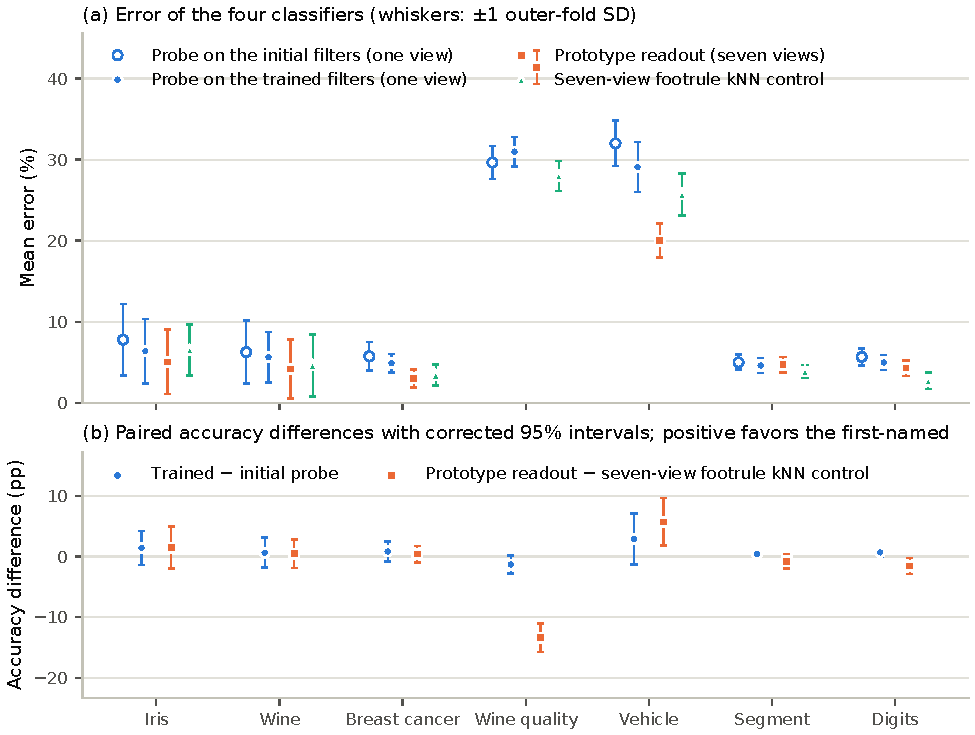
\includegraphics[width=\textwidth]{figures/data/fig7_learning_controls.pdf}
\caption{\textbf{Prototype-readout contrasts.} (a)~Mean outer-fold test error in percent on the seven benchmark datasets of four classifiers. A footrule kNN probe reads the hidden ranking of a single-view $[128]$ network before training (initial filters) and after training, with neighbor count and weighting chosen on inner folds (matched study). The others are the prototype readout with $K=7$ views and the seven-view footrule kNN control, footrule kNN on the same encoded views tuned on inner folds (component ablation). Whiskers are $\pm1$ outer-fold SD. (b)~The paired contrasts of Table~\ref{tab:contrasts}, trained minus initial probe and prototype readout minus kNN control, as accuracy differences in percentage points with 95\% corrected resampled-$t$ intervals (not simultaneous); positive favors the first-named. The prototype readout is at or above the kNN control on four datasets and below it on three. The trained probe is above the initial probe on six, and none of the seven probe intervals excludes zero. After Holm adjustment, one of the 14 contrasts remains significant (Wine quality prototype readout).}
\label{fig:learning-controls}
\end{figure}

% Rendered by render_tables.py from run files; do not edit by hand.
\begin{table}[!htbp]
\caption{\textbf{The 14 prototype-readout contrasts, fixed in the benchmark protocol before its outer folds were scored.} Paired accuracy differences in percentage points (first-named minus second-named; positive favors the first) on the seven benchmark datasets. Prototype readout $-$ seven-view footrule kNN control: the prototype readout with $K=7$ views against the seven-view footrule kNN control, footrule kNN on each of the same encoded views, tuned on inner folds and combined by majority vote (component ablation). Trained $-$ initial probe: a footrule kNN probe on the hidden ranking of the trained single-view $[128]$ network against the same probe on its initial filters (matched study). Each difference carries the 95\% corrected resampled-$t$ interval (test-to-training ratio 0.25, 14 degrees of freedom); intervals are not simultaneous, $p$ values are approximate, and the Holm column adjusts them over the family of 14. The prototype readout is at or above the kNN control on four datasets and the trained probe above the initial probe on six; three of the 14 intervals exclude zero, and one of the 14 contrasts remains significant after Holm adjustment.}
\label{tab:contrasts}
\centering
\footnotesize
\setlength{\tabcolsep}{3pt}
\begin{tabular}{lrrrr}
\toprule
Dataset & Difference (pp) & 95\% interval & $p$ & Holm $p$ \\
\midrule
\multicolumn{5}{l}{\emph{Prototype readout $-$ seven-view footrule kNN control}} \\
Iris & +1.5 & [$-$2.0, +4.9] & 0.374 & 1.000 \\
Wine & +0.4 & [$-$1.9, +2.8] & 0.693 & 1.000 \\
Breast cancer & +0.4 & [$-$1.0, +1.7] & 0.543 & 1.000 \\
Wine quality & $-$13.4 & [$-$15.7, $-$11.1] & $<$0.001 & $<$0.001 \\
Vehicle & +5.7 & [+1.8, +9.7] & 0.008 & 0.102 \\
Segment & $-$0.8 & [$-$2.0, +0.4] & 0.175 & 1.000 \\
Digits & $-$1.6 & [$-$2.9, $-$0.3] & 0.023 & 0.270 \\
\midrule
\multicolumn{5}{l}{\emph{Trained $-$ initial probe}} \\
Iris & +1.4 & [$-$1.4, +4.2] & 0.299 & 1.000 \\
Wine & +0.6 & [$-$1.9, +3.1] & 0.601 & 1.000 \\
Breast cancer & +0.8 & [$-$0.8, +2.5] & 0.292 & 1.000 \\
Wine quality & $-$1.3 & [$-$2.8, +0.2] & 0.081 & 0.810 \\
Vehicle & +2.9 & [$-$1.3, +7.1] & 0.160 & 1.000 \\
Segment & +0.4 & [$-$0.2, +1.0] & 0.168 & 1.000 \\
Digits & +0.7 & [$-$0.0, +1.4] & 0.059 & 0.654 \\
\bottomrule
\end{tabular}
\end{table}


The matched study looks at single-view networks in more detail. Table~\ref{tab:s-matched} reports the matched study on the seven benchmark datasets at every architecture. Table~\ref{tab:s-matched-controls} gives the reference classifiers on the same single encoded view. One of them, the hyperdimensional computing (HDC) control, is never trained. It works with bipolar vectors, whose entries are $+1$ and $-1$, in three steps. First, each item gets a fixed random bipolar key and each position a fixed bipolar code, nearby positions sharing most coordinates. Second, a ranking becomes the normalized sum over its positions of item key times position code. Third, each class vector is the normalized mean of its training vectors, and a query takes the class of highest cosine similarity. Cosine similarity is the cosine of the angle between two vectors. Nothing else is fitted.

Table~\ref{tab:s-contrasts} is the complete record of the 14 contrasts fixed in the prototype-readout protocol before its outer folds were scored. The matched protocol also declares its own family of 14 contrasts, two per dataset, with its own Holm adjustment. They set the trained probe against the initial one, and the prototype readout of the single-view network against fixed-configuration input footrule kNN. Table~\ref{tab:s-matched-family} reports this family for completeness, and no claim of this paper rests on it.

% Rendered by render_tables.py from run files; do not edit by hand.
\begin{table}[!htbp]
\caption{\textbf{Matched learning controls at every architecture (single view).} Mean outer-fold error in percent (outer-fold SD) on the seven benchmark datasets for the network's own prototype readout and for footrule kNN probes, tuned symmetrically on inner folds. The probes are applied to the hidden ranking of layer 1 and of the last hidden layer, of the trained network and of the same network before training (initial filters). One view per dataset, with learning rate 0.1, no augmentation and 200 iterations of batch size 32. Its encoder has degree $p=3$ with $e=16$ on Iris, $p=1$ with $e=64$ on Digits and $p=2$ with $e=32$ on the other five datasets. The validation fraction is 0.1 (the network trains on the remaining rows of each partition; probes and reference classifiers use every row). Protocol \texttt{arrowflow-v3-matched-1}.}
\label{tab:s-matched}
\centering
\scriptsize
\setlength{\tabcolsep}{3pt}
\resizebox{\ifdim\width>\linewidth\linewidth\else\width\fi}{!}{%
\begin{tabular}{llrrrrr}
\toprule
Dataset & Widths & Prototype readout & Probe, trained L1 & Probe, initial L1 & Probe, trained last & Probe, initial last \\
\midrule
Iris & $[128]$ & 11.2 (5.4) & 6.4 (4.0) & 7.8 (4.4) & (= layer 1) & (= layer 1) \\
 & $[64,128]$ & 10.7 (3.4) & 8.0 (4.3) & 7.9 (4.0) & 7.4 (4.1) & 8.1 (3.8) \\
 & $[64,32]$ & 9.3 (4.0) & 8.1 (4.5) & 8.3 (4.7) & 6.9 (3.4) & 9.3 (5.0) \\
\midrule
Wine & $[128]$ & 9.4 (4.1) & 5.6 (3.1) & 6.2 (3.9) & (= layer 1) & (= layer 1) \\
 & $[64,128]$ & 8.5 (5.6) & 7.2 (3.4) & 7.1 (3.2) & 6.1 (4.1) & 7.6 (3.9) \\
 & $[64,32]$ & 7.7 (3.3) & 6.7 (3.8) & 6.2 (3.7) & 6.2 (2.9) & 9.3 (3.3) \\
\midrule
Breast cancer & $[128]$ & 5.0 (1.5) & 4.9 (1.1) & 5.7 (1.8) & (= layer 1) & (= layer 1) \\
 & $[64,128]$ & 5.8 (1.5) & 5.7 (1.6) & 5.7 (1.6) & 5.1 (1.1) & 5.4 (1.2) \\
 & $[64,32]$ & 5.9 (1.6) & 5.4 (2.0) & 5.5 (1.9) & 5.3 (1.4) & 6.4 (2.0) \\
\midrule
Wine quality & $[128]$ & 48.8 (2.2) & 31.0 (1.8) & 29.6 (2.0) & (= layer 1) & (= layer 1) \\
 & $[64,128]$ & 49.7 (2.5) & 30.3 (2.1) & 29.7 (2.0) & 31.4 (1.7) & 29.9 (2.1) \\
 & $[64,32]$ & 49.8 (2.8) & 30.0 (2.2) & 29.9 (2.2) & 31.4 (1.9) & 30.4 (2.3) \\
\midrule
Vehicle & $[128]$ & 36.9 (2.4) & 29.1 (3.1) & 32.0 (2.8) & (= layer 1) & (= layer 1) \\
 & $[64,128]$ & 38.2 (3.0) & 32.6 (2.8) & 32.5 (2.7) & 32.9 (1.6) & 33.7 (3.5) \\
 & $[64,32]$ & 41.0 (2.7) & 32.7 (3.0) & 32.7 (3.1) & 34.0 (2.6) & 36.2 (3.2) \\
\midrule
Segment & $[128]$ & 12.1 (1.7) & 4.6 (0.9) & 5.0 (0.9) & (= layer 1) & (= layer 1) \\
 & $[64,128]$ & 12.7 (1.3) & 5.6 (1.1) & 5.3 (0.9) & 5.7 (1.0) & 5.6 (1.1) \\
 & $[64,32]$ & 14.5 (1.9) & 5.4 (1.0) & 5.3 (1.0) & 6.8 (1.1) & 7.0 (1.2) \\
\midrule
Digits & $[128]$ & 10.9 (1.5) & 5.0 (0.9) & 5.7 (1.1) & (= layer 1) & (= layer 1) \\
 & $[64,128]$ & 15.7 (0.9) & 7.1 (1.1) & 7.1 (1.0) & 8.2 (0.9) & 8.7 (1.4) \\
 & $[64,32]$ & 23.9 (2.4) & 7.1 (1.1) & 6.7 (1.2) & 13.8 (1.1) & 15.9 (1.1) \\
\bottomrule
\end{tabular}
}
\end{table}

% Rendered by render_tables.py from run files; do not edit by hand.
\begin{table}[!htbp]
\caption{\textbf{Reference classifiers on the same single encoded view.} Mean outer-fold error in percent (outer-fold SD) of the reference classifiers, each receiving the same encoded view as the networks of Table~\ref{tab:s-matched}. The first is fixed-configuration input footrule kNN: footrule kNN on the input rankings of this encoded view, with neighbors and weights tuned on inner folds. The others are the mean-position prototype classifier (one Borda prototype per class, nearest by footrule) and an ordered-position hyperdimensional computing (HDC) control. The HDC control has dimension 1,024 or 10,000, chosen on inner folds. Footrule kNN has the lowest error of the three on every dataset.}
\label{tab:s-matched-controls}
\centering
\footnotesize
\setlength{\tabcolsep}{3pt}
\begin{tabular}{lrrr}
\toprule
Dataset & Fixed-configuration input footrule kNN & Borda prototype & HDC \\
\midrule
Iris & 7.6 (5.3) & 16.4 (6.6) & 12.4 (6.7) \\
Wine & 6.6 (4.0) & 9.9 (5.3) & 7.2 (4.5) \\
Breast cancer & 5.6 (2.6) & 9.0 (2.4) & 9.0 (2.1) \\
Wine quality & 29.0 (2.4) & 49.1 (3.1) & 46.8 (2.7) \\
Vehicle & 31.3 (3.0) & 51.5 (3.4) & 50.9 (3.5) \\
Segment & 4.8 (0.8) & 21.5 (2.7) & 18.2 (2.1) \\
Digits & 4.3 (1.2) & 16.3 (2.0) & 13.8 (2.1) \\
\bottomrule
\end{tabular}
\end{table}


In Tables~\ref{tab:s-matched} and~\ref{tab:s-matched-controls}, at the primary architecture $[128]$ the network's prototype readout has lower error than footrule kNN on the input rankings only on Breast cancer ($5.0$ against $5.6\%$). On the other six datasets its error is higher, by $2.8$ (Wine) to $19.7$ points (Wine quality). On Wine quality, Segment and Digits, the prototype readout has $48.8$, $12.1$ and $10.9\%$ error. The trained probe on its hidden ranking has $31.0$, $4.6$ and $5.0\%$, and footrule kNN on the input rankings has $29.0$, $4.8$ and $4.3\%$. There the probe's error is within $2.0$ points of that of footrule kNN on the input rankings, a descriptive difference. The prototype readout has higher error than both. In Table~\ref{tab:s-matched}, the lowest prototype-readout error comes from $[128]$ on five datasets and from $[64,32]$ on Iris and Wine.

For the two-layer networks, we can also probe each hidden layer. The probe on the trained last hidden layer has error at most equal to that of the probe on the initial one in 11 of 14 pairs of dataset and architecture. The exceptions are Wine quality (both architectures) and Segment ($[64,128]$). The probe on the trained last hidden layer has higher error than the probe on the trained first layer on Wine quality, Vehicle, Segment and Digits at both two-layer architectures, and lower error on Iris, Wine and Breast cancer.

% Rendered by render_tables.py from run files; do not edit by hand.
\begin{table}[!htbp]
\caption{\textbf{Complete record of the 14 contrasts fixed in the benchmark protocol before its outer folds were scored.} Family index, dataset, contrast, source family, mean paired accuracy difference in percentage points, its standard error (SE) in points, the 95\% corrected resampled-$t$ interval (test-to-training ratio 0.25, 14 degrees of freedom), the approximate $p$ value and the Holm-adjusted $p$ value over the family of 14. Every member is computed, and one Holm adjustment covers the family.}
\label{tab:s-contrasts}
\centering
\scriptsize
\setlength{\tabcolsep}{3pt}
\resizebox{\ifdim\width>\linewidth\linewidth\else\width\fi}{!}{%
\begin{tabular}{rlllrrrrr}
\toprule
\# & Dataset & Contrast & Source & Diff. (pp) & SE & 95\% interval & $p$ & Holm $p$ \\
\midrule
1 & Iris & Prototype readout $-$ seven-view footrule kNN control & component ablation & +1.5 & 1.6 & [$-$2.0, +4.9] & 0.374 & 1.000 \\
2 & Wine & Prototype readout $-$ seven-view footrule kNN control & component ablation & +0.4 & 1.1 & [$-$1.9, +2.8] & 0.693 & 1.000 \\
3 & Breast cancer & Prototype readout $-$ seven-view footrule kNN control & component ablation & +0.4 & 0.6 & [$-$1.0, +1.7] & 0.543 & 1.000 \\
4 & Wine quality & Prototype readout $-$ seven-view footrule kNN control & component ablation & $-$13.4 & 1.1 & [$-$15.7, $-$11.1] & $<$0.001 & $<$0.001 \\
5 & Vehicle & Prototype readout $-$ seven-view footrule kNN control & component ablation & +5.7 & 1.8 & [+1.8, +9.7] & 0.008 & 0.102 \\
6 & Segment & Prototype readout $-$ seven-view footrule kNN control & component ablation & $-$0.8 & 0.6 & [$-$2.0, +0.4] & 0.175 & 1.000 \\
7 & Digits & Prototype readout $-$ seven-view footrule kNN control & component ablation & $-$1.6 & 0.6 & [$-$2.9, $-$0.3] & 0.023 & 0.270 \\
\midrule
8 & Iris & Trained $-$ initial probe & matched study & +1.4 & 1.3 & [$-$1.4, +4.2] & 0.299 & 1.000 \\
9 & Wine & Trained $-$ initial probe & matched study & +0.6 & 1.2 & [$-$1.9, +3.1] & 0.601 & 1.000 \\
10 & Breast cancer & Trained $-$ initial probe & matched study & +0.8 & 0.8 & [$-$0.8, +2.5] & 0.292 & 1.000 \\
11 & Wine quality & Trained $-$ initial probe & matched study & $-$1.3 & 0.7 & [$-$2.8, +0.2] & 0.081 & 0.810 \\
12 & Vehicle & Trained $-$ initial probe & matched study & +2.9 & 2.0 & [$-$1.3, +7.1] & 0.160 & 1.000 \\
13 & Segment & Trained $-$ initial probe & matched study & +0.4 & 0.3 & [$-$0.2, +1.0] & 0.168 & 1.000 \\
14 & Digits & Trained $-$ initial probe & matched study & +0.7 & 0.3 & [$-$0.0, +1.4] & 0.059 & 0.654 \\
\bottomrule
\end{tabular}
}
\end{table}

% Rendered by render_tables.py from run files; do not edit by hand.
\begin{table}[!htbp]
\caption{\textbf{Contrast family of the matched protocol.} The matched protocol declared these fourteen contrasts, two per dataset, with one Holm adjustment over them. The first is the footrule kNN probe on the trained hidden ranking of the single-view $[128]$ network minus the same probe on its initial filters; the second is that network's prototype readout minus fixed-configuration input footrule kNN. Differences are in percentage points with the 95\% corrected resampled-$t$ interval (test-to-training ratio 0.25, 14 degrees of freedom); $p$ values are approximate. The probe contrasts equal those of Table~\ref{tab:s-contrasts}, whose family adjusts them together with the seven-view control instead. This family is reported for completeness, and no claim of this paper rests on it. Four of the fourteen contrasts remain significant after Holm adjustment, each a prototype readout below fixed-configuration input footrule kNN.}
\label{tab:s-matched-family}
\centering
\scriptsize
\setlength{\tabcolsep}{3pt}
\resizebox{\ifdim\width>\linewidth\linewidth\else\width\fi}{!}{%
\begin{tabular}{llrrrr}
\toprule
Dataset & Contrast & Difference (pp) & 95\% interval & $p$ & Holm $p$ \\
\midrule
Iris & Trained $-$ initial probe & +1.4 & [$-$1.4, +4.2] & 0.299 & 1.000 \\
 & Prototype readout $-$ fixed-configuration input footrule kNN & $-$3.6 & [$-$11.5, +4.2] & 0.338 & 1.000 \\
\midrule
Wine & Trained $-$ initial probe & +0.6 & [$-$1.9, +3.1] & 0.601 & 1.000 \\
 & Prototype readout $-$ fixed-configuration input footrule kNN & $-$2.8 & [$-$8.0, +2.4] & 0.265 & 1.000 \\
\midrule
Breast cancer & Trained $-$ initial probe & +0.8 & [$-$0.8, +2.5] & 0.292 & 1.000 \\
 & Prototype readout $-$ fixed-configuration input footrule kNN & +0.6 & [$-$1.9, +3.1] & 0.613 & 1.000 \\
\midrule
Wine quality & Trained $-$ initial probe & $-$1.3 & [$-$2.8, +0.2] & 0.081 & 0.729 \\
 & Prototype readout $-$ fixed-configuration input footrule kNN & $-$19.7 & [$-$22.9, $-$16.6] & $<$0.001 & $<$0.001 \\
\midrule
Vehicle & Trained $-$ initial probe & +2.9 & [$-$1.3, +7.1] & 0.160 & 1.000 \\
 & Prototype readout $-$ fixed-configuration input footrule kNN & $-$5.6 & [$-$8.3, $-$2.9] & $<$0.001 & 0.007 \\
\midrule
Segment & Trained $-$ initial probe & +0.4 & [$-$0.2, +1.0] & 0.168 & 1.000 \\
 & Prototype readout $-$ fixed-configuration input footrule kNN & $-$7.3 & [$-$9.3, $-$5.3] & $<$0.001 & $<$0.001 \\
\midrule
Digits & Trained $-$ initial probe & +0.7 & [$-$0.0, +1.4] & 0.059 & 0.594 \\
 & Prototype readout $-$ fixed-configuration input footrule kNN & $-$6.6 & [$-$8.7, $-$4.5] & $<$0.001 & $<$0.001 \\
\bottomrule
\end{tabular}
}
\end{table}


\clearpage
\subsection{Details for Section~\ref*{sec:motion-controls}: Matched Motion-Signal Controls}\label{supp:motion}

This subsection and the next hold the complete numerical record of the eight controlled experiments summarized in Sections~\ref{sec:motion-controls} and~\ref{sec:controlled}. Every one of them reuses the split seed, the fitting seeds and the outer and inner folds of the registered runs. So each contrast is paired fold by fold with the run it is compared against. None of them changes the seventeen-dataset results of Sections~\ref{supp:benchmark} and~\ref{supp:training}, which stand as registered.

Each family carries its own Holm adjustment over its own contrasts. Every rate pooled over folds, repeats and fitting seeds is descriptive. Pooled rates count the same test rows more than once, so none of them receives an interval or a test. Section~\ref{supp:reproducibility} gives the protocol file, the code revision and the commands of each family.

\paragraph{Design.} These arms, the controls of Section~\ref{sec:motion-controls}, ask whether the particular signal the output layer returns carries information, or whether movement of the same size would serve as well. On most datasets, a scrambled signal leaves the network less accurate than frozen filters, so the signal does carry information. The arms change only what reaches the hidden filters. They hold everything else fixed: the encoder family and its selection, the nearest-neighbor readout, the seven views, the folds and the fitting seeds. The iteration count stays fixed too, and so does the eligibility gate that decides which training rows are accepted. Each arm applies the gate's rule to its own prototype readout, so its gate decisions are recomputed, not replayed.

An unmodified arm is fitted through the same instrumentation wrapper with an identity transform, one that leaves every motion as it is. It has to reproduce the reference run's outer predictions on every fold and seed. This check shows that the wrapper itself has no effect on the fit.

The frozen arm never applies the accumulated motion to its hidden filters. It asks whether the hidden filters need to move at all, and it cannot say whether their particular movement makes a difference. The frozen arm is not the untrained ArrowFlow of Section~\ref{supp:training}. That control never trains any layer, so its training settings have no effect. It also selects its own configuration. The readout reads only the hidden layers, so the frozen arm predicts exactly as the untrained networks of the component ablation (Section~\ref{supp:ablation-arrowflow}). Its column of Table~\ref{tab:s-motion-family} therefore equals that variant's column of Table~\ref{tab:s-components-changes}. Those results existed before this protocol was frozen, so only the two scrambling arms were scored blind.

The permuted-alignment arm keeps every motion record with its magnitude and sign. But it reassigns each record by a random permutation of the layer's filter identities. So it changes only which filter receives each motion. The permutation is drawn anew for every layer and batch. A fixed permutation, the permutation analog of feedback alignment \citep{lillicrap2016random}, was not tested. Feedback alignment trains a neural network by sending its errors back through fixed random weights, where backpropagation would reuse the forward weights.

The random-direction arm changes the directions instead. An attracting vote pulls a filter toward the batch input, and a repelling vote pushes it away. The arm shuffles the signs of the nonzero votes among their slots, within each record, layer and batch. A slot is one filter that one example selects in one batch. The shuffle keeps exactly the slots, the vote mass (the total vote weight) per batch and layer, the vote magnitudes with their repeats and the counts of attraction and repulsion. Only the pairing of each filter with its direction is broken. The arm leaves the mix of attraction and repulsion alone on purpose, because a changed mix would confound the comparison.

The two scrambles differ in strength. About half of the nonzero votes attract, so the random-direction arm reverses the direction of about half of them. Permuted alignment instead moves almost every selected slot, zero votes included, to another filter. Table~\ref{tab:s-motion-statistics} records both rates per dataset and layer. It also gives the share of each run's slots that carry a vote and the share of ArrowFlow's votes that repel, which is about half on every dataset and layer.

Every arm keeps the class-filter target and the error gate. The controls therefore show that it makes a difference which filter each motion reaches and in which direction. But they do not tell apart information from the labels and structure that any consistent target would impose. A full permutation of the class labels is a different experiment and is not claimed here.

Table~\ref{tab:s-motion-family} holds the primary family, the three arms on all seventeen datasets. Its contrasts are Holm-adjusted across the datasets within each arm, and the arms are adjusted separately. The protocol declared this before its own outer folds were scored. As noted above, the frozen arm's results existed earlier. Table~\ref{tab:s-motion-scramble} compares each scramble with the frozen arm directly, a comparison the protocol did not declare. Post hoc, an exact one-sided signed-rank test \citep{demsar2006statistical} across the seventeen datasets supports both scrambles being less accurate than frozen filters ($p<0.001$ for each). Table~\ref{tab:s-motion-purity} gives the same-class purity of the last hidden ranking for the test and the training rows of every arm. Purity is the share of a row's nearest stored training rankings that carry its class, so it measures the neighborhoods that the readout reads. The purity table is descriptive and carries no test.

Table~\ref{tab:s-motion-single-layer} holds two further arms that train only the first, or only the last, hidden layer. When a fold selected one hidden layer, both arms equal the unmodified run by construction. So each row uses only the outer folds whose selection has two hidden layers. No dataset selected two hidden layers on every outer fold, and several selected them on none. These arms therefore sit outside the primary family and are not Holm-adjusted. Every row prints its fold count.

\paragraph{Results.} On most datasets, training makes the neighborhoods purer, and either scramble makes them less pure than frozen filters. ArrowFlow's neighborhoods are purer than those of the frozen arm on 13 of the 17 datasets, and the permuted-alignment and random-direction arms leave them less pure than the frozen arm on 15 and 14 of the 17. No arm differs detectably on HCV, where no model beats the majority class, and its purities are essentially unchanged. The two scrambling arms change the votes in different ways and by different amounts (Table~\ref{tab:s-motion-statistics}). So each is read against the frozen arm, and the two are not compared with each other.

\clearpage
% Rendered by render_tables.py from run files; do not edit by hand.
\begin{table}[!htbp]
\caption{\textbf{Matched motion-signal controls: the primary family.} ArrowFlow minus the control arm, accuracy, in percentage points, on the seventeen datasets. Fitting seeds are averaged within each outer fold; intervals are 95\% corrected resampled-$t$ interval (test-to-training ratio 0.25, 14 degrees of freedom). Positive favors ArrowFlow. Holm adjusts across the seventeen datasets within each arm, the three arms separately, as the run protocol declared before its own outer folds were scored. The frozen arm predicts exactly as the untrained networks of the component ablation (Table~\ref{tab:s-components-changes}), whose results existed before this protocol was frozen, so only the two scrambling arms were scored blind. The permuted-alignment arm is less accurate than the frozen arm on 16 of the 17 datasets and the random-direction arm on 14 of the 17. Holm adjustment leaves 3 datasets significant in the frozen filters arm, 5 in the permuted alignment arm and 3 in the random directions arm. kNN: nearest-neighbor classifier; HCV: hepatitis C virus.}
\label{tab:s-motion-family}
\centering
\scriptsize
\setlength{\tabcolsep}{3pt}
\resizebox{\ifdim\width>\linewidth\linewidth\else\width\fi}{!}{%
\begin{tabular}{lrrrrrr}
\toprule
Dataset & \begin{tabular}[b]{@{}r@{}}Frozen\\Diff. (pp)\end{tabular} & \begin{tabular}[b]{@{}r@{}}Frozen\\95\% interval\end{tabular} & \begin{tabular}[b]{@{}r@{}}Frozen\\Holm $p$\end{tabular} & \begin{tabular}[b]{@{}r@{}}Permuted\\Diff. (pp)\end{tabular} & \begin{tabular}[b]{@{}r@{}}Permuted\\95\% interval\end{tabular} & \begin{tabular}[b]{@{}r@{}}Permuted\\Holm $p$\end{tabular} \\
\midrule
Iris & +0.52 & [$-$1.68, +2.72] & 1.000 & +0.96 & [$-$1.06, +2.98] & 1.000 \\
Wine & +0.68 & [$-$2.06, +3.41] & 1.000 & +0.87 & [$-$1.36, +3.10] & 1.000 \\
Breast cancer & +0.84 & [$-$0.45, +2.13] & 1.000 & +0.78 & [$-$0.49, +2.05] & 1.000 \\
Wine quality & +0.02 & [$-$1.03, +1.08] & 1.000 & +0.51 & [$-$0.82, +1.83] & 1.000 \\
Vehicle & +3.61 & [+1.18, +6.05] & 0.093 & +6.69 & [+3.15, +10.23] & 0.018 \\
Segment & +1.20 & [+0.54, +1.86] & 0.023 & +1.40 & [+0.65, +2.16] & 0.020 \\
Digits & +0.15 & [$-$0.89, +1.19] & 1.000 & +1.17 & [+0.29, +2.06] & 0.156 \\
balance-scale & +5.35 & [+3.39, +7.31] & $<$0.001 & +6.97 & [+4.38, +9.55] & $<$0.001 \\
mfeat-zernike & +2.47 & [+1.45, +3.49] & 0.002 & +7.06 & [+5.75, +8.37] & $<$0.001 \\
ionosphere & +0.19 & [$-$2.99, +3.37] & 1.000 & +1.90 & [$-$0.93, +4.73] & 1.000 \\
vertebra-column & +0.65 & [$-$2.74, +4.03] & 1.000 & +1.18 & [$-$1.63, +3.99] & 1.000 \\
diabetes & $-$0.15 & [$-$1.71, +1.42] & 1.000 & +0.92 & [$-$0.38, +2.22] & 1.000 \\
banknote-authentication & $-$0.02 & [$-$0.25, +0.22] & 1.000 & +0.03 & [$-$0.05, +0.12] & 1.000 \\
qsar-biodeg & +1.26 & [+0.32, +2.21] & 0.159 & +2.12 & [+0.86, +3.37] & 0.037 \\
steel-plates-fault & +0.96 & [$-$1.04, +2.96] & 1.000 & +2.16 & [$-$0.38, +4.71] & 0.981 \\
climate-model-simulation-crashes & +0.06 & [$-$0.32, +0.44] & 1.000 & +0.16 & [$-$0.28, +0.61] & 1.000 \\
HCV & $-$0.02 & [$-$1.79, +1.76] & 1.000 & +0.17 & [$-$1.95, +2.29] & 1.000 \\
\bottomrule
\end{tabular}
}
\par\medskip
\resizebox{\ifdim\width>\linewidth\linewidth\else\width\fi}{!}{%
\begin{tabular}{lrrr}
\toprule
Dataset & \begin{tabular}[b]{@{}r@{}}Random\\Diff. (pp)\end{tabular} & \begin{tabular}[b]{@{}r@{}}Random\\95\% interval\end{tabular} & \begin{tabular}[b]{@{}r@{}}Random\\Holm $p$\end{tabular} \\
\midrule
Iris & +0.81 & [$-$1.36, +2.99] & 1.000 \\
Wine & +1.24 & [$-$0.44, +2.92] & 1.000 \\
Breast cancer & +0.74 & [$-$0.56, +2.04] & 1.000 \\
Wine quality & +0.33 & [$-$0.76, +1.41] & 1.000 \\
Vehicle & +6.49 & [+2.91, +10.07] & 0.024 \\
Segment & +1.42 & [+0.48, +2.36] & 0.079 \\
Digits & +0.34 & [$-$0.63, +1.31] & 1.000 \\
balance-scale & +6.35 & [+4.03, +8.67] & $<$0.001 \\
mfeat-zernike & +4.56 & [+3.27, +5.84] & $<$0.001 \\
ionosphere & +1.64 & [$-$0.92, +4.21] & 1.000 \\
vertebra-column & +0.57 & [$-$2.22, +3.36] & 1.000 \\
diabetes & +0.14 & [$-$1.59, +1.88] & 1.000 \\
banknote-authentication & +0.00 & [$-$0.23, +0.23] & 1.000 \\
qsar-biodeg & +1.86 & [+0.68, +3.04] & 0.062 \\
steel-plates-fault & +1.66 & [$-$0.63, +3.95] & 1.000 \\
climate-model-simulation-crashes & +0.16 & [$-$0.25, +0.58] & 1.000 \\
HCV & $-$0.14 & [$-$2.21, +1.92] & 1.000 \\
\bottomrule
\end{tabular}
}
\end{table}

% Rendered by render_tables.py from run files; do not edit by hand.
\begin{table}[!htbp]
\caption{\textbf{Matched motion-signal controls: each scramble against frozen filters (post hoc).} The mean accuracy of each scrambling arm minus that of the frozen arm, in percentage points, per dataset; negative means that the scrambled signal left the network less accurate than frozen filters. The values are differences of the arm accuracies of Table~\ref{tab:s-motion-family}, so they carry no interval. The protocol declared ArrowFlow minus each arm, not this comparison. The test ranks the seventeen absolute differences, and its $p$ value is the share of the $2^{17}$ sign assignments whose sum of positive ranks is at most the observed one. Post hoc, an exact one-sided Wilcoxon signed-rank test across the seventeen datasets gives $p=2.3\times10^{-5}$ for permuted alignment, below the frozen arm on 16 of the 17 datasets, and $p=3.3\times10^{-4}$ for random directions, below it on 14 of the 17. HCV: hepatitis C virus.}
\label{tab:s-motion-scramble}
\centering
\scriptsize
\setlength{\tabcolsep}{3pt}
\begin{tabular}{lrr}
\toprule
Dataset & \begin{tabular}[b]{@{}r@{}}Permuted\\$-$ frozen (pp)\end{tabular} & \begin{tabular}[b]{@{}r@{}}Random\\$-$ frozen (pp)\end{tabular} \\
\midrule
Iris & $-$0.44 & $-$0.30 \\
Wine & $-$0.19 & $-$0.56 \\
Breast cancer & +0.06 & +0.10 \\
Wine quality & $-$0.49 & $-$0.31 \\
Vehicle & $-$3.07 & $-$2.88 \\
Segment & $-$0.20 & $-$0.22 \\
Digits & $-$1.03 & $-$0.19 \\
balance-scale & $-$1.62 & $-$1.00 \\
mfeat-zernike & $-$4.59 & $-$2.09 \\
ionosphere & $-$1.70 & $-$1.45 \\
vertebra-column & $-$0.54 & +0.07 \\
diabetes & $-$1.07 & $-$0.29 \\
banknote-authentication & $-$0.05 & $-$0.02 \\
qsar-biodeg & $-$0.85 & $-$0.60 \\
steel-plates-fault & $-$1.20 & $-$0.70 \\
climate-model-simulation-crashes & $-$0.10 & $-$0.10 \\
HCV & $-$0.18 & +0.13 \\
\bottomrule
\end{tabular}
\end{table}

% Rendered by render_tables.py from run files; do not edit by hand.
\begin{table}[!htbp]
\caption{\textbf{Matched motion-signal controls: neighborhood purity.} Same-class purity of the last hidden ranking, in percent. For each row it is the share of its nearest stored training rankings that carry its class, at the neighbor count the view selected. Rows are averaged first, then the seven views, then the outer folds. Training rows drop their own stored ranking and are subsampled above 512 rows. Descriptive: no test and no interval. On balance-scale the purity of the outer test rows is 89.72 percent for ArrowFlow, 77.61 for the frozen filters, 73.85 for the permuted alignment and 75.17 for the random directions. HCV: hepatitis C virus.}
\label{tab:s-motion-purity}
\centering
\scriptsize
\setlength{\tabcolsep}{3pt}
\resizebox{\ifdim\width>\linewidth\linewidth\else\width\fi}{!}{%
\begin{tabular}{lrrrrrrrr}
\toprule
Dataset & \begin{tabular}[b]{@{}r@{}}ArrowFlow\\Test\end{tabular} & \begin{tabular}[b]{@{}r@{}}ArrowFlow\\Training\end{tabular} & \begin{tabular}[b]{@{}r@{}}Frozen\\Test\end{tabular} & \begin{tabular}[b]{@{}r@{}}Frozen\\Training\end{tabular} & \begin{tabular}[b]{@{}r@{}}Permuted\\Test\end{tabular} & \begin{tabular}[b]{@{}r@{}}Permuted\\Training\end{tabular} & \begin{tabular}[b]{@{}r@{}}Random\\Test\end{tabular} & \begin{tabular}[b]{@{}r@{}}Random\\Training\end{tabular} \\
\midrule
Iris & 92.10 & 92.69 & 91.59 & 91.91 & 90.44 & 90.67 & 90.99 & 91.36 \\
Wine & 94.15 & 95.58 & 90.68 & 91.13 & 92.64 & 93.31 & 91.90 & 92.32 \\
Breast cancer & 95.47 & 96.44 & 93.83 & 94.14 & 94.15 & 94.52 & 93.98 & 94.31 \\
Wine quality & 52.09 & 52.54 & 52.31 & 52.49 & 51.67 & 51.79 & 51.96 & 52.11 \\
Vehicle & 71.41 & 74.24 & 68.37 & 69.74 & 64.03 & 65.63 & 65.28 & 66.62 \\
Segment & 96.60 & 96.75 & 95.71 & 95.86 & 94.88 & 95.07 & 95.14 & 95.29 \\
Digits & 94.74 & 96.23 & 94.23 & 94.25 & 92.63 & 92.69 & 94.03 & 94.15 \\
balance-scale & 89.72 & 90.37 & 77.61 & 77.68 & 73.85 & 73.90 & 75.17 & 75.15 \\
mfeat-zernike & 78.13 & 79.25 & 75.22 & 74.90 & 69.18 & 68.99 & 72.28 & 72.04 \\
ionosphere & 86.05 & 88.18 & 85.66 & 86.51 & 83.54 & 84.89 & 83.97 & 84.89 \\
vertebra-column & 76.57 & 77.80 & 74.99 & 75.23 & 74.64 & 75.19 & 74.95 & 75.22 \\
diabetes & 67.29 & 67.83 & 67.21 & 67.47 & 66.73 & 67.12 & 66.89 & 67.19 \\
banknote-authentication & 99.54 & 99.62 & 99.46 & 99.53 & 99.43 & 99.49 & 99.48 & 99.55 \\
qsar-biodeg & 79.83 & 79.88 & 79.30 & 79.04 & 78.89 & 78.75 & 79.22 & 79.04 \\
steel-plates-fault & 66.39 & 67.79 & 66.93 & 67.46 & 64.29 & 64.65 & 65.86 & 66.24 \\
climate-model-simulation-crashes & 85.43 & 86.58 & 87.13 & 87.29 & 86.63 & 86.73 & 86.80 & 86.94 \\
HCV & 24.92 & 28.05 & 24.95 & 26.36 & 24.94 & 25.73 & 24.92 & 25.84 \\
\bottomrule
\end{tabular}
}
\end{table}

% Rendered by render_tables.py from run files; do not edit by hand.
\begin{table}[!htbp]
\caption{\textbf{Matched motion-signal controls: what each arm changed.} Counts over every fold, seed and view, per dataset and hidden layer; layer 1 is the first hidden layer. A slot is one filter that one example selects in one batch: every example of every batch selects $\lceil\rho N_\ell\rceil$ filters of each hidden layer, and an example that the gate rejects gives its slots zero votes. Selected slots: their number in millions, the same in every arm. Nonzero: the share of the selected slots that carry a nonzero vote, in the arm's own run. Repulsions: the share of ArrowFlow's nonzero votes that push a filter away from the batch input rather than pull it toward it. Moved: the share of all selected slots, zero votes included, that permuted alignment delivers to another filter. Reversed: the share of the random-direction arm's nonzero votes whose direction it reverses; permuting the signs of votes of which a share $q$ attract reverses a share $2q(1-q)$ on average. Both arms preserve the slots, the vote magnitudes and the vote mass of every batch exactly. Among ArrowFlow's nonzero votes, repulsions make up about half, 49.87 to 50.12 percent, on every dataset and layer, and the random-direction arm reverses 49.74 to 49.90 percent of its nonzero votes. On balance-scale permuted alignment moves 99.23 percent of the selected slots to another filter, and random directions reverses 49.87 percent of its nonzero votes, which are 17.67 percent of the selected slots, so the two arms are not equally strong.}
\label{tab:s-motion-statistics}
\centering
\scriptsize
\setlength{\tabcolsep}{3pt}
\begin{tabular}{llrrrrrr}
\toprule
Dataset & Layer & \begin{tabular}[b]{@{}r@{}}Selected\\slots (M)\end{tabular} & \begin{tabular}[b]{@{}r@{}}ArrowFlow:\\nonzero (\%)\end{tabular} & \begin{tabular}[b]{@{}r@{}}ArrowFlow:\\repulsions (\%)\end{tabular} & \begin{tabular}[b]{@{}r@{}}Permuted:\\moved (\%)\end{tabular} & \begin{tabular}[b]{@{}r@{}}Random:\\nonzero (\%)\end{tabular} & \begin{tabular}[b]{@{}r@{}}Random:\\reversed (\%)\end{tabular} \\
\midrule
Iris & 1 & 98.9 & 4.00 & 49.98 & 98.99 & 6.84 & 49.81 \\
Iris & 2 & 60.2 & 4.27 & 50.08 & 99.22 & 7.34 & 49.80 \\
\midrule
Wine & 1 & 81.7 & 1.94 & 50.01 & 98.76 & 4.24 & 49.77 \\
Wine & 2 & 94.6 & 2.11 & 50.01 & 99.22 & 4.54 & 49.85 \\
\midrule
Breast cancer & 1 & 111.8 & 3.63 & 49.98 & 99.10 & 4.51 & 49.83 \\
Breast cancer & 2 & 34.4 & 4.12 & 50.06 & 99.22 & 5.07 & 49.89 \\
\midrule
Wine quality & 1 & 129.0 & 54.30 & 49.87 & 99.21 & 47.98 & 49.86 \\
\midrule
Vehicle & 1 & 116.1 & 36.81 & 49.99 & 99.13 & 41.55 & 49.86 \\
Vehicle & 2 & 25.8 & 30.70 & 50.12 & 99.21 & 40.36 & 49.88 \\
\midrule
Segment & 1 & 129.0 & 15.40 & 50.05 & 99.22 & 27.28 & 49.85 \\
\midrule
Digits & 1 & 129.0 & 10.02 & 50.07 & 99.22 & 38.78 & 49.86 \\
\midrule
balance-scale & 1 & 129.0 & 10.47 & 50.08 & 99.23 & 17.67 & 49.87 \\
\midrule
mfeat-zernike & 1 & 129.0 & 26.65 & 50.06 & 99.22 & 54.70 & 49.87 \\
\midrule
ionosphere & 1 & 111.8 & 15.50 & 50.00 & 99.10 & 19.11 & 49.85 \\
ionosphere & 2 & 34.4 & 31.73 & 50.07 & 99.22 & 24.04 & 49.90 \\
\midrule
vertebra-column & 1 & 81.7 & 21.97 & 50.01 & 98.77 & 21.58 & 49.74 \\
vertebra-column & 2 & 94.6 & 21.70 & 50.05 & 99.23 & 21.66 & 49.77 \\
\midrule
diabetes & 1 & 107.5 & 41.45 & 49.94 & 99.06 & 33.70 & 49.86 \\
diabetes & 2 & 43.0 & 47.65 & 50.02 & 99.23 & 34.50 & 49.88 \\
\midrule
banknote-authentication & 1 & 90.3 & 4.49 & 50.01 & 98.88 & 6.27 & 49.76 \\
banknote-authentication & 2 & 77.4 & 5.31 & 50.02 & 99.23 & 7.11 & 49.82 \\
\midrule
qsar-biodeg & 1 & 129.0 & 33.91 & 49.94 & 99.22 & 28.75 & 49.85 \\
\midrule
steel-plates-fault & 1 & 129.0 & 40.09 & 50.03 & 99.22 & 53.77 & 49.87 \\
\midrule
climate-model-simulation-crashes & 1 & 107.5 & 35.41 & 50.01 & 99.06 & 34.89 & 49.85 \\
climate-model-simulation-crashes & 2 & 43.0 & 31.02 & 50.05 & 99.22 & 33.66 & 49.87 \\
\midrule
HCV & 1 & 81.7 & 66.92 & 49.93 & 98.76 & 70.69 & 49.77 \\
HCV & 2 & 94.6 & 67.66 & 50.08 & 99.22 & 70.96 & 49.88 \\
\bottomrule
\end{tabular}
\end{table}

% Rendered by render_tables.py from run files; do not edit by hand.
\begin{table}[!htbp]
\caption{\textbf{Matched motion-signal controls: one hidden layer trained.} ArrowFlow minus an arm in which only the first, or only the last, hidden layer applies its accumulated motion, accuracy, in percentage points. At a one-hidden-layer selection the arm is ArrowFlow by construction, so each row uses only the outer folds whose selection has two hidden layers; the second column gives their number $n$. Intervals are 95\% corrected resampled-$t$ intervals over the $n$ folds of a row, with the variance of the fold differences multiplied by $1/n+0.25$ and $n-1$ degrees of freedom; the $p$ values use the same $t$ distribution. Every fold difference is zero in the last-only row of climate-model-simulation-crashes, which therefore has no interval and no test. Descriptive: not part of the primary family and not Holm-adjusted. Seven of the seventeen datasets selected two hidden layers on no outer fold, so their rows are empty.}
\label{tab:s-motion-single-layer}
\centering
\scriptsize
\setlength{\tabcolsep}{3pt}
\resizebox{\ifdim\width>\linewidth\linewidth\else\width\fi}{!}{%
\begin{tabular}{llrrrrrr}
\toprule
Dataset & \begin{tabular}[b]{@{}r@{}}Two-layer\\folds\end{tabular} & \begin{tabular}[b]{@{}r@{}}First only\\Diff. (pp)\end{tabular} & \begin{tabular}[b]{@{}r@{}}First only\\95\% interval\end{tabular} & \begin{tabular}[b]{@{}r@{}}First only\\$p$\end{tabular} & \begin{tabular}[b]{@{}r@{}}Last only\\Diff. (pp)\end{tabular} & \begin{tabular}[b]{@{}r@{}}Last only\\95\% interval\end{tabular} & \begin{tabular}[b]{@{}r@{}}Last only\\$p$\end{tabular} \\
\midrule
Iris & 7 of 15 & +0.32 & [$-$1.30, +1.94] & 0.649 & $-$0.32 & [$-$1.61, +0.97] & 0.569 \\
Wine & 11 of 15 & +1.61 & [$-$1.26, +4.48] & 0.240 & +0.00 & [$-$1.33, +1.33] & 0.997 \\
Breast cancer & 4 of 15 & +0.36 & [$-$2.29, +3.02] & 0.691 & $-$0.22 & [$-$2.12, +1.68] & 0.735 \\
Wine quality & 0 of 15 & -- & -- & -- & -- & -- & -- \\
Vehicle & 3 of 15 & +1.37 & [$-$6.68, +9.42] & 0.540 & $-$2.23 & [$-$4.52, +0.06] & 0.052 \\
Segment & 0 of 15 & -- & -- & -- & -- & -- & -- \\
Digits & 0 of 15 & -- & -- & -- & -- & -- & -- \\
balance-scale & 0 of 15 & -- & -- & -- & -- & -- & -- \\
mfeat-zernike & 0 of 15 & -- & -- & -- & -- & -- & -- \\
ionosphere & 4 of 15 & $-$0.36 & [$-$4.11, +3.39] & 0.782 & $-$0.95 & [$-$2.70, +0.80] & 0.182 \\
vertebra-column & 11 of 15 & +0.34 & [$-$2.90, +3.58] & 0.819 & $-$0.49 & [$-$2.53, +1.55] & 0.605 \\
diabetes & 5 of 15 & +0.09 & [$-$2.89, +3.06] & 0.938 & +0.44 & [$-$2.39, +3.26] & 0.690 \\
banknote-authentication & 9 of 15 & $-$0.04 & [$-$0.39, +0.31] & 0.795 & $-$0.09 & [$-$0.37, +0.18] & 0.453 \\
qsar-biodeg & 0 of 15 & -- & -- & -- & -- & -- & -- \\
steel-plates-fault & 0 of 15 & -- & -- & -- & -- & -- & -- \\
climate-model-simulation-crashes & 5 of 15 & $-$0.06 & [$-$0.32, +0.20] & 0.541 & +0.00 & -- & -- \\
HCV & 11 of 15 & +1.47 & [$-$0.77, +3.70] & 0.174 & +0.19 & [$-$2.61, +2.98] & 0.885 \\
\bottomrule
\end{tabular}
}
\end{table}


\clearpage
\subsection{Details for Section~\ref*{sec:controlled}: What Training Does and Where It Stops}\label{supp:controlled}

This subsection looks inside the trained networks and tests the limits of the approach. The general remarks at the start of Section~\ref{supp:motion} apply to the seven studies below. Each paragraph carries the question of the main-text paragraph it supports.

\paragraph{What does training teach the network?} These analyses ask where the two largest training gains, on balance-scale and mfeat-zernike, come from. In balance-scale, each row places a weight at some distance on each side of a balance. The class says whether the balance tips left, tips right or stays level. Most of what training adds on this dataset comes from the rare balanced class. The analyses are descriptive and post hoc, and they read predictions that already existed. No model is refitted, and no interval is computed from a pooled count. Table~\ref{tab:s-mech-class-rates} gives per-class recall on balance-scale for every model of the benchmark. It also gives the number of fitting seeds, the number of outer fits and the number of rows of each class. A deterministic model, one whose fit does not depend on a random seed, is fitted at one seed. So it contributes a third of the rows of a stochastic one, and that is why the table prints those counts.

Tables~\ref{tab:s-mech-ladder-balance} and~\ref{tab:s-mech-ladder-mfeat} place the ordinal pipeline on a ladder from numeric nearest neighbors on the raw features to ArrowFlow, with the recall of each class at every rung. Neighboring rungs differ in more than one component, so the ladder cannot assign a gain to any single component. The torque of a side is its weight times its distance, and the rule that generated the dataset compares the two torques. Table~\ref{tab:s-mech-torque} groups the balance-scale rows by the absolute difference of the two torques and gives each model's recall in each bucket. That the rule reproduces every label is an arithmetic fact about the dataset. It says nothing about the network. The analysis shows only where the gain sits, and it leaves open whether the network recovered the rule.

Table~\ref{tab:s-mech-reading} splits the mfeat-zernike error into what sorting costs and what random filters cost, and it states how much of that cost training returns. It also records how often ArrowFlow and the untrained control selected the same architecture. That count discloses that the two contrasts surviving the post hoc adjustment over all thirty-four training contrasts do not compare the same architecture on every fold. On mfeat-zernike the reading differs from balance-scale. There, training recovers most of what sorting and random filters cost, without reaching the accuracy of numeric kNN on the projected scores before sorting.

\clearpage
% Rendered by render_tables.py from run files; do not edit by hand.
\begin{table}[!htbp]
\caption{\textbf{Mechanism: per-class recall on balance-scale.} Share of the rows of each class that the model returns, in percent, pooled over the outer folds, repeats and fitting seeds. The three classes are the balanced scale (B), and the tips to the left (L) and to the right (R). The row count of a deterministic model is a third of a stochastic model's, because it is fitted at one seed. Descriptive: the pooled rows repeat the same underlying test rows, so no rate here carries an interval or a test. ArrowFlow returns the balanced class on 52.381 percent of its 441 balanced-class rows, the untrained ArrowFlow on 2.721, tuned input footrule kNN on 4.082 and numeric kNN on the projected scores on 0.227. A tuned support vector classifier, fitted at one seed, returns the balanced class on 95.238 percent of its 147 balanced-class rows.}
\label{tab:s-mech-class-rates}
\centering
\scriptsize
\setlength{\tabcolsep}{3pt}
\resizebox{\ifdim\width>\linewidth\linewidth\else\width\fi}{!}{%
\begin{tabular}{lrrrrrrrr}
\toprule
Model & Seeds & Fits & \begin{tabular}[b]{@{}r@{}}Balanced\\rows\end{tabular} & \begin{tabular}[b]{@{}r@{}}Balanced\\recall (\%)\end{tabular} & \begin{tabular}[b]{@{}r@{}}Left\\rows\end{tabular} & \begin{tabular}[b]{@{}r@{}}Left\\recall (\%)\end{tabular} & \begin{tabular}[b]{@{}r@{}}Right\\rows\end{tabular} & \begin{tabular}[b]{@{}r@{}}Right\\recall (\%)\end{tabular} \\
\midrule
ArrowFlow & 3 & 45 & 441 & 52.381 & 2,592 & 97.878 & 2,592 & 97.145 \\
Untrained ArrowFlow & 3 & 45 & 441 & 2.721 & 2,592 & 96.759 & 2,592 & 95.910 \\
Tuned input footrule kNN & 3 & 45 & 441 & 4.082 & 2,592 & 96.103 & 2,592 & 96.489 \\
Numeric kNN, projected scores & 3 & 45 & 441 & 0.227 & 2,592 & 97.415 & 2,592 & 97.299 \\
SVC (RBF) & 1 & 15 & 147 & 95.238 & 864 & 97.917 & 864 & 98.380 \\
MLP & 3 & 45 & 441 & 92.971 & 2,592 & 98.187 & 2,592 & 98.341 \\
Random forest & 3 & 45 & 441 & 0.000 & 2,592 & 93.519 & 2,592 & 93.634 \\
Gradient boosting & 3 & 45 & 441 & 0.000 & 2,592 & 99.306 & 2,592 & 99.421 \\
Numeric kNN & 1 & 15 & 147 & 0.000 & 864 & 97.569 & 864 & 97.222 \\
Majority class & 1 & 15 & 147 & 0.000 & 864 & 59.722 & 864 & 39.583 \\
\bottomrule
\end{tabular}
}
\end{table}

% Rendered by render_tables.py from run files; do not edit by hand.
\begin{table}[!htbp]
\caption{\textbf{Mechanism: the representation ladder on balance-scale.} Mean outer-fold error in percent (outer-fold SD) of the five rungs, and the recall of each class in percent, pooled over the outer folds, repeats and fitting seeds. Neighboring rungs differ in more than one component. Descriptive: the pooled recalls repeat the same test rows, so none of them carries an interval or a test.}
\label{tab:s-mech-ladder-balance}
\centering
\scriptsize
\setlength{\tabcolsep}{3pt}
\resizebox{\ifdim\width>\linewidth\linewidth\else\width\fi}{!}{%
\begin{tabular}{lrrrrr}
\toprule
Rung & Seeds & \begin{tabular}[b]{@{}r@{}}Error \%\\(SD)\end{tabular} & Balanced & Left & Right \\
\midrule
Numeric kNN on the raw features & 1 & 10.2 (1.5) & 0.0 & 97.6 & 97.2 \\
Numeric kNN on the projected scores & 3 & 10.3 (1.2) & 0.2 & 97.4 & 97.3 \\
Tuned input footrule kNN & 3 & 10.9 (1.5) & 4.1 & 96.1 & 96.5 \\
The untrained ArrowFlow & 3 & 11.0 (1.3) & 2.7 & 96.8 & 95.9 \\
ArrowFlow & 3 & 6.0 (1.3) & 52.4 & 97.9 & 97.1 \\
\bottomrule
\end{tabular}
}
\end{table}

% Rendered by render_tables.py from run files; do not edit by hand.
\begin{table}[!htbp]
\caption{\textbf{Mechanism: the representation ladder on mfeat-zernike.} Mean outer-fold error in percent (outer-fold SD) of the five rungs, and the recall of each class in percent, pooled over the outer folds, repeats and fitting seeds. Neighboring rungs differ in more than one component. Descriptive: the pooled recalls repeat the same test rows, so none of them carries an interval or a test.}
\label{tab:s-mech-ladder-mfeat}
\centering
\scriptsize
\setlength{\tabcolsep}{3pt}
\resizebox{\ifdim\width>\linewidth\linewidth\else\width\fi}{!}{%
\begin{tabular}{lrrrrrrrrrrrr}
\toprule
Rung & Seeds & \begin{tabular}[b]{@{}r@{}}Error \%\\(SD)\end{tabular} & 1 & 2 & 3 & 4 & 5 & 6 & 7 & 8 & 9 & 10 \\
\midrule
Numeric kNN on the raw features & 1 & 19.6 (1.7) & 96.3 & 96.0 & 96.0 & 86.0 & 94.3 & 82.7 & 29.5 & 95.3 & 92.5 & 34.8 \\
Numeric kNN on the projected scores & 3 & 19.0 (1.4) & 96.7 & 96.3 & 97.2 & 86.2 & 96.2 & 85.6 & 24.8 & 95.7 & 93.7 & 37.8 \\
Tuned input footrule kNN & 3 & 21.5 (1.2) & 97.8 & 96.9 & 94.2 & 82.1 & 95.8 & 74.4 & 28.7 & 97.8 & 92.0 & 25.3 \\
The untrained ArrowFlow & 3 & 21.6 (1.4) & 97.6 & 97.2 & 95.2 & 82.1 & 96.3 & 73.6 & 26.2 & 97.6 & 92.0 & 26.1 \\
ArrowFlow & 3 & 19.3 (1.0) & 97.8 & 97.1 & 96.7 & 85.0 & 97.2 & 79.6 & 34.4 & 96.2 & 95.4 & 27.6 \\
\bottomrule
\end{tabular}
}
\end{table}

% Rendered by render_tables.py from run files; do not edit by hand.
\begin{table}[!htbp]
\caption{\textbf{Mechanism: balance-scale recall by torque gap.} Recall in percent within each bucket of $|\Delta|$, the absolute difference of the two torques (weight $\times$ distance); $\Delta = 0$ is exactly the balanced class. The header counts the distinct test rows of the bucket; each is predicted once per outer fold and fitting seed. Descriptive: pooled rates over repeated rows, with no interval and no test. The physical rule is read from the four features and is not learned by any model here. The rule reproduces the label of all 625 balance-scale rows, and the 49 rows of the balanced bucket carry 219 of the 280 extra correct predictions ArrowFlow makes over the untrained ArrowFlow.}
\label{tab:s-mech-torque}
\centering
\scriptsize
\setlength{\tabcolsep}{3pt}
\resizebox{\ifdim\width>\linewidth\linewidth\else\width\fi}{!}{%
\begin{tabular}{lrrrrr}
\toprule
Model & \begin{tabular}[b]{@{}r@{}}$|\Delta| = 0$\\49 rows\end{tabular} & \begin{tabular}[b]{@{}r@{}}$|\Delta| = 1$ to $2$\\116 rows\end{tabular} & \begin{tabular}[b]{@{}r@{}}$|\Delta| = 3$ to $5$\\144 rows\end{tabular} & \begin{tabular}[b]{@{}r@{}}$|\Delta| = 6$ to $10$\\162 rows\end{tabular} & \begin{tabular}[b]{@{}r@{}}$|\Delta| \geq 11$\\154 rows\end{tabular} \\
\midrule
ArrowFlow & 52.4 & 87.6 & 100.0 & 100.0 & 100.0 \\
Untrained ArrowFlow & 2.7 & 84.6 & 97.8 & 100.0 & 100.0 \\
Tuned input footrule kNN & 4.1 & 83.0 & 98.8 & 100.0 & 100.0 \\
Numeric kNN, projected scores & 0.2 & 87.2 & 99.8 & 100.0 & 100.0 \\
SVC (RBF) & 95.2 & 90.8 & 100.0 & 100.0 & 100.0 \\
MLP & 93.0 & 91.4 & 100.0 & 100.0 & 100.0 \\
Random forest & 0.0 & 75.6 & 94.0 & 100.0 & 100.0 \\
Gradient boosting & 0.0 & 97.1 & 99.8 & 100.0 & 100.0 \\
Numeric kNN & 0.0 & 87.4 & 99.8 & 100.0 & 100.0 \\
Majority class & 0.0 & 51.7 & 48.8 & 48.6 & 50.0 \\
\bottomrule
\end{tabular}
}
\end{table}

% Rendered by render_tables.py from run files; do not edit by hand.
\begin{table}[!htbp]
\caption{\textbf{Mechanism: where the error goes, and which architecture was selected.} The first block gives mean outer-fold error in percent and the differences between neighboring rungs in points; a positive difference is a cost paid, and the training line is what training gives back. The last three lines of the block are the paired ArrowFlow minus projected kNN difference with its 95\% corrected resampled-$t$ interval (test-to-training ratio 0.25, 14 degrees of freedom), post hoc and unadjusted. The second block counts outer folds. On mfeat-zernike sorting costs 2.5056 points and random layers 0.1556, and training returns 2.3389 of the 2.6611 points. The untrained control chose two hidden layers on 2 of the 15 balance-scale and 1 of the 15 mfeat-zernike outer folds.}
\label{tab:s-mech-reading}
\centering
\scriptsize
\setlength{\tabcolsep}{3pt}
\begin{tabular}{lrr}
\toprule
Quantity & balance-scale & mfeat-zernike \\
\midrule
\multicolumn{3}{l}{\emph{Error and its differences (percent, points)}} \\
Numeric kNN on the raw features & 10.2400 & 19.6500 \\
Numeric kNN on the projected scores & 10.2578 & 18.9722 \\
Tuned input footrule kNN & 10.9333 & 21.4778 \\
Untrained ArrowFlow & 11.0044 & 21.6333 \\
ArrowFlow & 6.0267 & 19.2944 \\
Sorting cost: input $-$ projected & 0.6756 & 2.5056 \\
Random layers: untrained $-$ input & 0.0711 & 0.1556 \\
Representation cost: untrained $-$ projected & 0.7467 & 2.6611 \\
Training returns: untrained $-$ ArrowFlow & 4.9778 & 2.3389 \\
ArrowFlow $-$ projected, accuracy (pp) & +4.2311 & $-$0.3222 \\
95\% interval of that difference & [+2.92, +5.54] & [$-$1.39, +0.75] \\
$p$ of that difference, unadjusted & $<$0.001 & 0.529 \\
\midrule
\multicolumn{3}{l}{\emph{Selected architecture (outer folds)}} \\
Outer folds & 15 & 15 \\
ArrowFlow chose two hidden layers on & 0 & 0 \\
The untrained control chose two hidden layers on & 2 & 1 \\
Both chose the same widths on & 13 & 14 \\
\bottomrule
\end{tabular}
\end{table}


\paragraph{Do the filters move at all?} These diagnostics ask whether training moves the filters, and they measure how ties limit the layers. The filters do move. None of the 1,785 views of one fitting seed returned its initial filters (Table~\ref{tab:s-diag-checkpoints}). The tables describe how the fitted networks behave. Nothing is selected and nothing is fitted. A read-only wrapper records what happens inside the registered ArrowFlow run. It draws no random numbers and leaves the network state unchanged. Every check passed on every job:
\begin{itemize}[leftmargin=2em,topsep=2pt,itemsep=1pt]
\item The instrumented fit reproduces the saved outer predictions.
\item An uninstrumented fit reproduces the recorded state hashes.
\item The checkpoint rule matches the core exactly.
\item The forward pass is reimplemented independently.
\end{itemize}
A post-processing module then reads the frozen result files and builds the tables below. It fits nothing.

Four definitions fix what the tables mean. First, the checkpoint is the update at which the validation error of the prototype readout was lowest, so checkpoint zero would mean that a view returned its initial filters (Table~\ref{tab:s-diag-checkpoints}). Second, displacement is the footrule distance between a filter's initial and checkpointed order, normalized by the maximum $\lfloor V^2/2 \rfloor$ for a permutation of $V$ items. So it runs from 0 for an unchanged filter to 1 for the largest possible change. Under the same normalization the reference for two independent uniform permutations is $\bigl((V^2-1)/3\bigr)/\lfloor V^2/2\rfloor$, about $2/3$. That is the displacement expected between two orders drawn at random. Views whose checkpoint is zero are excluded, because their displacement is zero by definition (Table~\ref{tab:s-diag-displacement}).

Third, a tied response is a pair of filters at equal footrule distance from the input. The filter identities then decide the order of such a pair. That distance is an even integer in a bounded range, so the number of values a response can take grows with the permutation length alone. Tie shares are therefore reported by permutation length, beside a simulated reference with uniform random filters (Tables~\ref{tab:s-diag-ties} and~\ref{tab:s-diag-output-ties}). Fourth, relabeling permutes the filter identities of a layer and relabels the next layer's vocabulary to match. This leaves every distance untouched and changes only how ties are broken. The share of seven-view predictions that relabeling changes measures how much the tie-breaking convention affects the predictions (Table~\ref{tab:s-diag-relabel}).

The learning curves of Figure~\ref{fig:learning-curves} start at update zero, with the initial filters. For the nearest-neighbor readouts, the first point also uses the readout setting that the fit chose after training. So these first points never compare trained filters with untrained ones. That comparison comes from the component ablation of Section~\ref{supp:ablations}.

The checkpoint comes early on the smallest datasets, where its median is update 6 on Iris and update 2 on Wine, judged on 12 and 14 validation rows (Table~\ref{tab:s-diag-checkpoints}). The tie shares of Table~\ref{tab:s-diag-ties} mean that hidden rankings contain many small groups of tied filters, and the filter identities set the order inside each group. At $V=32$ with 128 filters the number of distinct responses is less than half the number of filters, so a group holds about two filters on average. For uniform random filters only about 1.4 percent of filter pairs tie there (Section~\ref{supp:margin}), so the identities decide few pairwise comparisons. Relabeling changes the most seven-view predictions on HCV (Table~\ref{tab:s-diag-relabel}), and HCV's negative training estimate should be read in that light.

\clearpage
% Rendered by render_tables.py from run files; do not edit by hand.
\begin{table}[!htbp]
\caption{\textbf{Training diagnostics: checkpoints.} Every dataset contributes 15 outer folds $\times$ seven views $= 105$ views, each trained for 200 updates. The checkpoint is the last update whose error on the core's held-out validation rows is strictly below the running minimum before it; zero means the core returned the initial filters. Quartiles are over all views of the group. Descriptive: one fitting seed, nothing selected. No view returned its initial filters: none of the 1,785 views has checkpoint zero, and the median checkpoint runs from 2 on Wine to 146 on Segment of 200 updates. HCV: hepatitis C virus.}
\label{tab:s-diag-checkpoints}
\centering
\scriptsize
\setlength{\tabcolsep}{3pt}
\begin{tabular}{lrrrrr}
\toprule
Dataset & \begin{tabular}[b]{@{}r@{}}Validation\\rows\end{tabular} & \begin{tabular}[b]{@{}r@{}}Views with\\checkpoint 0\end{tabular} & \begin{tabular}[b]{@{}r@{}}Median\\checkpoint\end{tabular} & Q1 & Q3 \\
\midrule
Iris & 12 & 0 & 6 & 3 & 8 \\
Wine & 14 & 0 & 2 & 1 & 7 \\
Breast cancer & 45 & 0 & 11 & 5 & 24 \\
Wine quality & 127--128 & 0 & 96 & 48 & 130 \\
Vehicle & 67 & 0 & 134 & 83 & 168 \\
Segment & 184 & 0 & 146 & 116 & 168 \\
Digits & 143 & 0 & 133 & 89 & 162 \\
balance-scale & 50 & 0 & 79 & 56 & 115 \\
mfeat-zernike & 160 & 0 & 138 & 113 & 167 \\
ionosphere & 28 & 0 & 42 & 17 & 97 \\
vertebra-column & 24 & 0 & 26 & 13 & 62 \\
diabetes & 61 & 0 & 82 & 43 & 133 \\
banknote-authentication & 109 & 0 & 33 & 17 & 77 \\
qsar-biodeg & 84 & 0 & 102 & 57 & 155 \\
steel-plates-fault & 155 & 0 & 131 & 91 & 163 \\
climate-model-simulation-crashes & 43 & 0 & 118 & 71 & 168 \\
HCV & 110 & 0 & 80 & 38 & 135 \\
\midrule
All seventeen together & 12--184 & 0 & 79 & 21 & 137 \\
\bottomrule
\end{tabular}
\end{table}

% Rendered by render_tables.py from run files; do not edit by hand.
\begin{table}[!htbp]
\caption{\textbf{Training diagnostics: displacement at the checkpoint.} Per view, the mean over the filters of a layer of the footrule distance between the checkpoint filter and its initial filter, divided by the largest footrule $\lfloor V^2/2 \rfloor$, where $V$ is the number of items the layer orders. Hidden layers are numbered from one. Rows pool every view of every dataset with that architecture and $V$. The reference $\bigl((V^2-1)/3\bigr)/\lfloor V^2/2 \rfloor$ is the expected normalized footrule between two independent uniform permutations. Descriptive. In the single-hidden-layer networks the mean displacement at the checkpoint runs from 0.443 to 0.521, against 0.664 to 0.667 for two independent uniform permutations.}
\label{tab:s-diag-displacement}
\centering
\scriptsize
\setlength{\tabcolsep}{3pt}
\begin{tabular}{llrrrrrr}
\toprule
Widths & Layer & $V$ & Views & Mean & SD & \begin{tabular}[b]{@{}r@{}}Filters\\changed (\%)\end{tabular} & \begin{tabular}[b]{@{}r@{}}Random\\reference\end{tabular} \\
\midrule
$[128]$ & Hidden 1 & 16 & 112 & 0.521 & 0.118 & 99.9 & 0.664 \\
$[128]$ & Hidden 1 & 32 & 364 & 0.492 & 0.143 & 99.9 & 0.666 \\
$[128]$ & Hidden 1 & 64 & 567 & 0.499 & 0.110 & 100.0 & 0.667 \\
$[128]$ & Hidden 1 & 128 & 252 & 0.443 & 0.107 & 100.0 & 0.667 \\
$[128]$ & Output & 128 & 1295 & 0.296 & 0.172 & 99.9 & 0.667 \\
$[64,128]$ & Hidden 1 & 16 & 147 & 0.084 & 0.116 & 57.6 & 0.664 \\
$[64,128]$ & Hidden 1 & 32 & 217 & 0.090 & 0.094 & 94.2 & 0.666 \\
$[64,128]$ & Hidden 1 & 64 & 105 & 0.152 & 0.115 & 100.0 & 0.667 \\
$[64,128]$ & Hidden 1 & 128 & 21 & 0.206 & 0.164 & 100.0 & 0.667 \\
$[64,128]$ & Hidden 2 & 64 & 490 & 0.461 & 0.137 & 100.0 & 0.667 \\
$[64,128]$ & Output & 128 & 490 & 0.301 & 0.155 & 100.0 & 0.667 \\
\bottomrule
\end{tabular}
\end{table}

% Rendered by render_tables.py from run files; do not edit by hand.
\begin{table}[!htbp]
\caption{\textbf{Training diagnostics: response ties of the hidden layers.} Share of the responses on the outer test rows that another filter of the same layer attains exactly, and the mean share of distinct responses among the $N$ filters of a row; hidden layers are numbered from one. The random column reads uniform random filters of the same shape through the same forward pass and the same tie definition, over 200 filter sets. A footrule between permutations of $V$ items is even and at most $\lfloor V^2/2 \rfloor$, so a response takes at most the last column's number of values. Descriptive. At the first hidden layer of a $[128]$ network ordering 32 items the tied-response share is 0.787 at the initial filters, 0.811 at the checkpoint and 0.788 for uniform random filters.}
\label{tab:s-diag-ties}
\centering
\scriptsize
\setlength{\tabcolsep}{3pt}
\resizebox{\ifdim\width>\linewidth\linewidth\else\width\fi}{!}{%
\begin{tabular}{llrrrrrrrrr}
\toprule
Widths & Layer & $V$ & $N$ & \begin{tabular}[b]{@{}r@{}}Tied\\initial\end{tabular} & \begin{tabular}[b]{@{}r@{}}Tied\\checkpoint\end{tabular} & \begin{tabular}[b]{@{}r@{}}Tied\\random\end{tabular} & \begin{tabular}[b]{@{}r@{}}Distinct\\initial\end{tabular} & \begin{tabular}[b]{@{}r@{}}Distinct\\checkpoint\end{tabular} & \begin{tabular}[b]{@{}r@{}}Distinct\\random\end{tabular} & \begin{tabular}[b]{@{}r@{}}Distinct\\values\end{tabular} \\
\midrule
$[128]$ & Hidden 1 & 16 & 128 & 0.950 & 0.960 & 0.950 & 0.241 & 0.212 & 0.239 & 65 \\
$[128]$ & Hidden 1 & 32 & 128 & 0.787 & 0.811 & 0.788 & 0.485 & 0.443 & 0.484 & 257 \\
$[128]$ & Hidden 1 & 64 & 128 & 0.464 & 0.520 & 0.464 & 0.739 & 0.697 & 0.740 & 1,025 \\
$[128]$ & Hidden 1 & 128 & 128 & 0.204 & 0.248 & 0.205 & 0.893 & 0.869 & 0.893 & 4,097 \\
$[64,128]$ & Hidden 1 & 16 & 64 & 0.866 & 0.854 & 0.865 & 0.395 & 0.410 & 0.397 & 65 \\
$[64,128]$ & Hidden 1 & 32 & 64 & 0.569 & 0.550 & 0.573 & 0.669 & 0.682 & 0.667 & 257 \\
$[64,128]$ & Hidden 1 & 64 & 64 & 0.273 & 0.255 & 0.272 & 0.855 & 0.866 & 0.856 & 1,025 \\
$[64,128]$ & Hidden 1 & 128 & 64 & 0.105 & 0.074 & 0.109 & 0.946 & 0.962 & 0.944 & 4,097 \\
$[64,128]$ & Hidden 2 & 64 & 128 & 0.466 & 0.433 & 0.464 & 0.739 & 0.754 & 0.740 & 1,025 \\
\bottomrule
\end{tabular}
}
\end{table}

% Rendered by render_tables.py from run files; do not edit by hand.
\begin{table}[!htbp]
\caption{\textbf{Training diagnostics: ties at the output layer.} Share of outer test rows whose smallest response is attained by more than one class filter, at the initial filters and at the checkpoint. Rows group the views by architecture and class count, since the output layer holds one filter per class. Descriptive.}
\label{tab:s-diag-output-ties}
\centering
\scriptsize
\setlength{\tabcolsep}{3pt}
\begin{tabular}{lrrrrr}
\toprule
Widths & Classes & Datasets & Views & \begin{tabular}[b]{@{}r@{}}Tied nearest,\\initial\end{tabular} & \begin{tabular}[b]{@{}r@{}}Tied nearest,\\checkpoint\end{tabular} \\
\midrule
$[128]$ & 2 & 6 & 441 & 0.0020 & 0.0023 \\
$[128]$ & 3 & 5 & 322 & 0.0025 & 0.0022 \\
$[128]$ & 4 & 2 & 112 & 0.0035 & 0.0023 \\
$[128]$ & 7 & 2 & 210 & 0.0048 & 0.0019 \\
$[128]$ & 10 & 2 & 210 & 0.0046 & 0.0007 \\
$[64,128]$ & 2 & 5 & 189 & 0.0014 & 0.0015 \\
$[64,128]$ & 3 & 3 & 203 & 0.0021 & 0.0010 \\
$[64,128]$ & 4 & 2 & 98 & 0.0030 & 0.0053 \\
\bottomrule
\end{tabular}
\end{table}

% Rendered by render_tables.py from run files; do not edit by hand.
\begin{table}[!htbp]
\caption{\textbf{Training diagnostics: sensitivity to filter-ID tie-breaking.} At inference on the checkpoint network the hidden filter identities are permuted, with the next layer relabeled to match; the output layer is not relabeled. Each view and each seven-view majority is drawn 20 times. Columns give the share of outer test predictions that change, in percent, and the smallest and largest change of the seven-view accuracy in percentage points. Descriptive: one fitting seed, so its accuracy differs from the three-seed accuracy behind Table~\ref{tab:main} by up to 1.0 points. Relabeling changes under 0.31 percent of the seven-view predictions on 10 of the 17 datasets and 21.11 percent on HCV. HCV: hepatitis C virus.}
\label{tab:s-diag-relabel}
\centering
\scriptsize
\setlength{\tabcolsep}{3pt}
\resizebox{\ifdim\width>\linewidth\linewidth\else\width\fi}{!}{%
\begin{tabular}{lrrrrrrr}
\toprule
Dataset & \begin{tabular}[b]{@{}r@{}}Accuracy\\(\%)\end{tabular} & \begin{tabular}[b]{@{}r@{}}View:\\mean (\%)\end{tabular} & \begin{tabular}[b]{@{}r@{}}View:\\max (\%)\end{tabular} & \begin{tabular}[b]{@{}r@{}}Majority:\\mean (\%)\end{tabular} & \begin{tabular}[b]{@{}r@{}}Majority:\\max (\%)\end{tabular} & \begin{tabular}[b]{@{}r@{}}Accuracy\\change min\end{tabular} & \begin{tabular}[b]{@{}r@{}}Accuracy\\change max\end{tabular} \\
\midrule
Iris & 94.0 & 0.35 & 10.00 & 0.20 & 6.67 & +0.00 & +6.67 \\
Wine & 96.4 & 0.24 & 8.33 & 0.05 & 2.86 & +0.00 & +2.86 \\
Breast cancer & 97.3 & 0.12 & 3.51 & 0.13 & 1.75 & $-$0.88 & +1.75 \\
Wine quality & 72.3 & 1.49 & 5.00 & 1.46 & 3.44 & $-$2.19 & +1.88 \\
Vehicle & 80.4 & 2.11 & 13.53 & 1.96 & 8.24 & $-$2.96 & +2.37 \\
Segment & 97.4 & 0.15 & 0.87 & 0.09 & 0.87 & $-$0.43 & +0.22 \\
Digits & 97.3 & 0.10 & 1.11 & 0.06 & 0.56 & $-$0.28 & +0.56 \\
balance-scale & 94.5 & 0.41 & 4.00 & 0.29 & 1.60 & $-$0.80 & +1.60 \\
mfeat-zernike & 81.0 & 0.70 & 3.75 & 0.81 & 2.50 & $-$1.00 & +1.00 \\
ionosphere & 88.8 & 0.24 & 4.29 & 0.28 & 1.43 & $-$1.43 & +1.43 \\
vertebra-column & 83.1 & 2.69 & 14.52 & 2.70 & 11.29 & $-$3.23 & +6.45 \\
diabetes & 75.8 & 2.32 & 12.42 & 2.20 & 8.44 & $-$3.25 & +2.60 \\
banknote-authentication & 99.8 & 0.05 & 2.91 & 0.00 & 0.00 & +0.00 & +0.00 \\
qsar-biodeg & 87.6 & 0.32 & 2.84 & 0.30 & 1.42 & $-$0.95 & +0.95 \\
steel-plates-fault & 75.1 & 1.32 & 5.14 & 1.32 & 4.88 & $-$1.55 & +1.29 \\
climate-model-simulation-crashes & 91.6 & 0.31 & 5.56 & 0.03 & 0.93 & $-$0.93 & +0.93 \\
HCV & 24.0 & 12.48 & 37.18 & 21.11 & 44.40 & $-$6.50 & +4.33 \\
\bottomrule
\end{tabular}
}
\end{table}

% Figure S5: learning curves. Rendered by render_tables.py via render_figures.learning_curves from the sealed
% report-ready tables of the training diagnostics; nothing numeric is typed here.
\begin{figure}[!htbp]
\centering
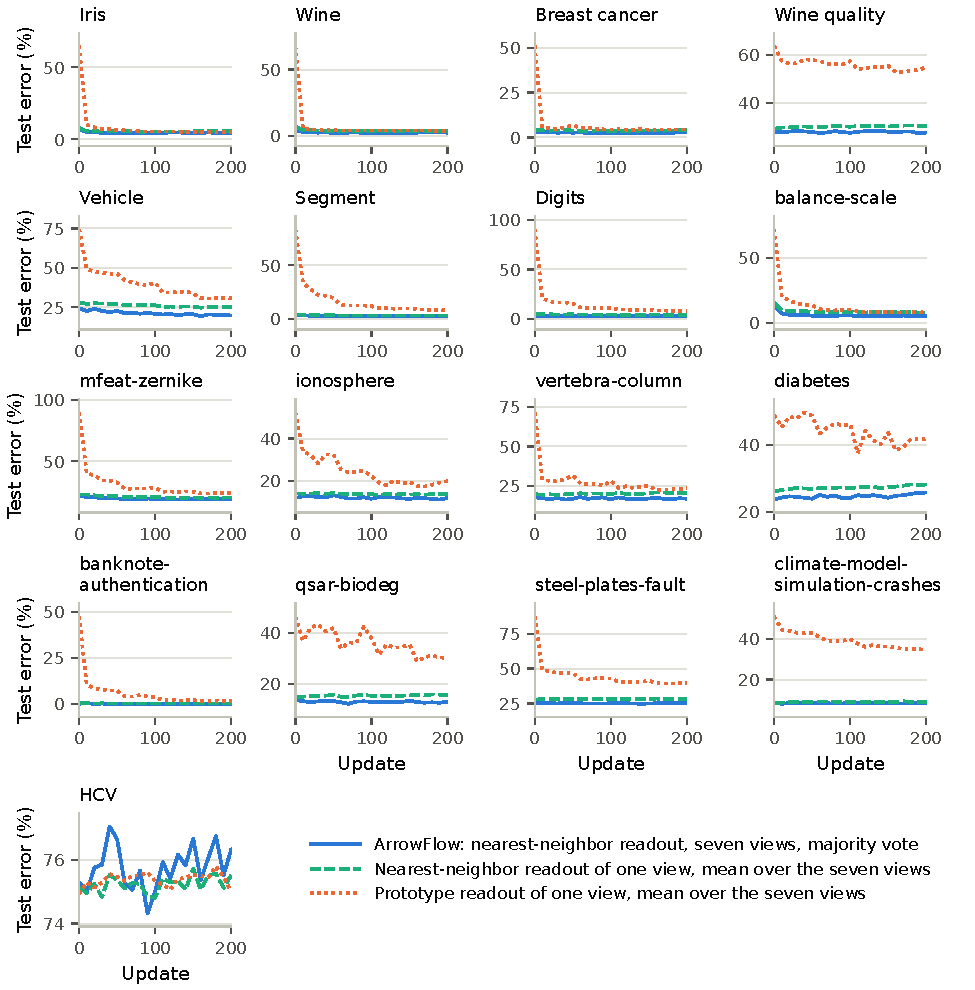
\includegraphics[width=\textwidth]{figures/data/figS_learning_curves.pdf}
\caption{\textbf{Training diagnostics: learning curves.} Test error in percent on the outer test rows against the number of updates, every ten updates from the initial filters, update 0, to update 200, for one fitting seed; each point is the mean over the 15 outer folds. Solid: ArrowFlow's seven-view nearest-neighbor readout, combined by majority vote. Dashed: the nearest-neighbor readout of one view, and dotted: the prototype readout of one view, each averaged over the seven views. The curves follow the filters through training, while the network that ArrowFlow returns is the one at its checkpoint (Table~\ref{tab:s-diag-checkpoints}). Each panel has its own error scale. Descriptive: nothing is selected or tested. At update 200 the prototype readout of one view has higher test error than the nearest-neighbor readout of one view on 15 of the 17 datasets. HCV: hepatitis C virus.}
\label{fig:learning-curves}
\end{figure}


Post hoc and descriptively, these diagnostics and the component ablation suggest three reasons why the training gain is modest. First, the prototype readout drives the gate, the returned signal and the checkpoint. Yet it has higher error than even the untrained networks read by nearest neighbors on 11 of the 17 datasets (Table~\ref{tab:s-components-errors}). Its advantage over those networks tracks ArrowFlow's gain over them, with a Spearman correlation of 0.50 over the 17 datasets. Second, on Iris, Wine, Breast cancer and banknote-authentication only 1.9 to 5.3 percent of the selected slots carry a vote, against at least 10.0 percent on every other dataset (Table~\ref{tab:s-motion-statistics}). So training there has little to work with. Third, on Vehicle, Segment, Digits, mfeat-zernike and steel-plates-fault the median checkpoint is update 131 to 146 of 200, so at least half of the views there still improved their validation error after update 130 (Table~\ref{tab:s-diag-checkpoints}).

\paragraph{Does a second hidden layer help?} Two families ask whether a second hidden layer earns its place, holding everything else at the configuration the fold itself selected. It did not help in either family. The first, the fixed-configuration depth family, ran with the earlier relay. The second repeats its primary contrast with the corrected relay of Section~\ref{sec:training}.

The first family holds fixed the fold, the encoder settings, the learning rate, the iteration count and the readout. It varies the hidden widths and, in two further arms, how much of the stack is trained. Table~\ref{tab:s-depth-contrasts} gives the three contrasts, each Holm-adjusted across the seventeen datasets. The primary contrast sets one trained hidden layer against two trained hidden layers. The other two arms are weakened on purpose. The untrained-second arm adds a second hidden layer and never trains it, and the first-only arm trains the first hidden layer only.

Table~\ref{tab:s-depth-movement} gives, for each arm, the share of its hidden filters that a batch update reorders, and it must be read beside Table~\ref{tab:s-depth-contrasts}. This is a rate per update over the whole fit. It differs from the displacement of Table~\ref{tab:s-diag-displacement}, which compares each filter's initial and checkpointed orders once. So a filter that few updates reorder can still end far from where it began. Freezing the second layer also quiets the first. As a result, part of a weakened arm's deficit comes from less adaptation, and the extra layer does not explain all of it. Pooled over all folds, both fully trained depths reorder a similar share of their hidden filters per update, the two-layer networks at least nine tenths as many as the one-layer networks, although the ratio varies by dataset. One hidden layer is more accurate than the untrained-second arm on 15 of the 17 datasets, but that arm reorders less than a third as many filters as the fully trained two-layer arm. Table~\ref{tab:s-depth-subsets} repeats the primary contrast on the folds that selected one hidden layer and on those that selected two.

The second family, depth with the corrected relay, reuses the one-layer arm and the two-layer arm with the earlier relay of the first family. As a check, a refit of the first outer fold of every dataset reproduced both exactly. The family fits two new two-layer arms on the same folds, seed and settings: one with the corrected relay, and one whose first-layer votes are also multiplied by 8. The scale tests a second reason why the first layer may learn little. Its votes may be too weak to overcome the prior, the identity term of the accumulator that votes for the filter's current order. Equation~\eqref{eq:signal} keeps a relayed signal below $cV_\ell$, so a first-layer vote stays below $2\eta c$. After every batch reset, the prior dictates a filter's order while its batch vote mass stays below $1/(e-1)$ (Section~\ref{supp:iia}). The scale 8 is the smallest of 1, 2, 4, 8, 16 and 32 at which at least half of the first layer's voted filter-batches reach that threshold, on training-only pilot fits of Iris and ionosphere. The protocol fixed the reading in advance. By its rule, a corrected arm helps only if it is ahead of one hidden layer on at least 9 of the 17 datasets and significantly ahead, after Holm adjustment, on at least one.

Neither corrected arm helps (Table~\ref{tab:s-relay-contrasts}). One hidden layer is more accurate than two with the corrected relay on 9 of the 17 datasets, by $+0.24$ points on average, and than the scaled arm on 14. No contrast of either arm survives Holm adjustment. The correction itself makes two-layer networks more accurate than the earlier relay on 12 of the 17 datasets, by $+0.64$ points on average, again with no Holm-significant contrast. The scaled votes reorder the first layer's filters far more often, in 81.6 against 34.5 percent of the updates on average, without making two layers more accurate (Table~\ref{tab:s-relay-movement}).

Both families run one fitting seed per fold and retune neither the learning rate nor the iteration count. So they show whether the second layer earns its place at the selected configuration. The best model attainable at either depth is a separate question, and the families say nothing about deeper stacks.

\clearpage
% Rendered by render_tables.py from run files; do not edit by hand.
\begin{table}[!htbp]
\caption{\textbf{Depth at a matched configuration.} One hidden layer minus each two-layer arm, accuracy, in percentage points with the 95\% corrected resampled-$t$ interval (test-to-training ratio 0.25, 14 degrees of freedom); positive favors one layer. Every arm reads the same per-fold selection, the same splits and one fitting seed, and neither the learning rate nor the update count is retuned. The untrained-second arm never moves its second hidden layer; the first-only arm never moves the layer the readout reads. Every two-layer arm used the earlier relay of Section~\ref{sec:training}; Table~\ref{tab:s-relay-contrasts} repeats the primary contrast with the corrected relay. Holm adjusts across the seventeen datasets within each arm. One hidden layer is more accurate than two on 15 of the 17 datasets at a matched configuration, none of the seventeen contrasts survives Holm adjustment, and the largest difference is mfeat-zernike +2.98 points (Holm 0.056). HCV: hepatitis C virus.}
\label{tab:s-depth-contrasts}
\centering
\scriptsize
\setlength{\tabcolsep}{3pt}
\resizebox{\ifdim\width>\linewidth\linewidth\else\width\fi}{!}{%
\begin{tabular}{lrrrrrr}
\toprule
Dataset & \begin{tabular}[b]{@{}r@{}}Two\\Diff. (pp) [interval]\end{tabular} & \begin{tabular}[b]{@{}r@{}}Two\\Holm $p$\end{tabular} & \begin{tabular}[b]{@{}r@{}}Untrained\\Diff. (pp) [interval]\end{tabular} & \begin{tabular}[b]{@{}r@{}}Untrained\\Holm $p$\end{tabular} & \begin{tabular}[b]{@{}r@{}}First\\Diff. (pp) [interval]\end{tabular} & \begin{tabular}[b]{@{}r@{}}First\\Holm $p$\end{tabular} \\
\midrule
Iris & +0.44 [$-$1.63, +2.52] & 1.000 & +1.33 [$-$2.00, +4.66] & 1.000 & +0.22 [$-$1.62, +2.06] & 1.000 \\
Wine & +0.37 [$-$1.80, +2.54] & 1.000 & +1.49 [$-$2.13, +5.12] & 1.000 & +0.17 [$-$3.58, +3.93] & 1.000 \\
Breast cancer & $-$0.29 [$-$1.78, +1.19] & 1.000 & +0.47 [$-$1.53, +2.46] & 1.000 & +0.70 [$-$1.27, +2.67] & 1.000 \\
Wine quality & +0.77 [$-$1.27, +2.81] & 1.000 & +0.54 [$-$1.46, +2.55] & 1.000 & +0.25 [$-$1.02, +1.52] & 1.000 \\
Vehicle & +2.96 [$-$0.51, +6.42] & 1.000 & +4.02 [$-$0.07, +8.10] & 0.697 & +4.89 [+1.97, +7.81] & 0.044 \\
Segment & +1.15 [+0.01, +2.30] & 0.717 & +1.18 [+0.06, +2.31] & 0.569 & +0.92 [$-$0.02, +1.87] & 0.764 \\
Digits & +0.63 [$-$0.60, +1.86] & 1.000 & +1.22 [+0.18, +2.27] & 0.373 & +1.21 [$-$0.07, +2.48] & 0.818 \\
balance-scale & +1.65 [+0.17, +3.13] & 0.499 & +7.04 [+4.40, +9.68] & $<$0.001 & +6.03 [+2.57, +9.49] & 0.035 \\
mfeat-zernike & +2.98 [+1.17, +4.79] & 0.056 & +6.33 [+4.59, +8.08] & $<$0.001 & +4.28 [+2.73, +5.84] & $<$0.001 \\
ionosphere & +1.05 [$-$2.24, +4.33] & 1.000 & +0.76 [$-$2.73, +4.24] & 1.000 & +1.42 [$-$1.69, +4.54] & 1.000 \\
vertebra-column & +0.22 [$-$3.60, +4.03] & 1.000 & +1.51 [$-$3.67, +6.68] & 1.000 & +0.11 [$-$3.05, +3.27] & 1.000 \\
diabetes & +1.87 [$-$0.39, +4.12] & 1.000 & +1.09 [$-$1.92, +4.09] & 1.000 & +1.22 [$-$1.55, +3.98] & 1.000 \\
banknote-authentication & +0.00 [$-$0.23, +0.24] & 1.000 & $-$0.10 [$-$0.71, +0.51] & 1.000 & $-$0.12 [$-$0.71, +0.47] & 1.000 \\
qsar-biodeg & +1.01 [$-$1.26, +3.28] & 1.000 & +1.42 [$-$1.36, +4.20] & 1.000 & +1.33 [$-$1.16, +3.81] & 1.000 \\
steel-plates-fault & +1.53 [$-$0.13, +3.19] & 0.957 & +1.39 [$-$0.17, +2.95] & 0.922 & +1.12 [$-$0.82, +3.06] & 1.000 \\
climate-model-simulation-crashes & +0.12 [$-$0.45, +0.70] & 1.000 & +0.19 [$-$0.28, +0.65] & 1.000 & +0.19 [$-$0.28, +0.65] & 1.000 \\
HCV & $-$1.44 [$-$5.18, +2.30] & 1.000 & $-$0.26 [$-$3.36, +2.83] & 1.000 & $-$0.94 [$-$4.53, +2.65] & 1.000 \\
\bottomrule
\end{tabular}
}
\end{table}

% Rendered by render_tables.py from run files; do not edit by hand.
\begin{table}[!htbp]
\caption{\textbf{Depth: how much each arm moved.} Share of the hidden filter updates that change the filter's order, in percent. Every batch updates each hidden filter once, and the share pools the batches, the hidden layers and the seven views of a fit and is averaged over the outer folds. It is a rate per update, not the displacement at the checkpoint of Table~\ref{tab:s-diag-displacement}. The last columns count the outer folds on which an arm is effectively inert, that is below a changed share of 0.01. The last row pools all 255 folds. A contrast against an arm that barely moves is evidence about movement, not about depth. Descriptive. Over all folds a hidden filter update reorders the filter in 67.8 and 63.8 percent of the cases in the two fully trained arms, in 13.3 percent in the untrained-second arm and in 18.4 percent in the first-only arm. HCV: hepatitis C virus.}
\label{tab:s-depth-movement}
\centering
\scriptsize
\setlength{\tabcolsep}{3pt}
\resizebox{\ifdim\width>\linewidth\linewidth\else\width\fi}{!}{%
\begin{tabular}{lrrrrrrr}
\toprule
Dataset & \begin{tabular}[b]{@{}r@{}}One\\changed (\%)\end{tabular} & \begin{tabular}[b]{@{}r@{}}Two\\changed (\%)\end{tabular} & \begin{tabular}[b]{@{}r@{}}Untrained\\changed (\%)\end{tabular} & \begin{tabular}[b]{@{}r@{}}First\\changed (\%)\end{tabular} & \begin{tabular}[b]{@{}r@{}}Two\\inert folds\end{tabular} & \begin{tabular}[b]{@{}r@{}}Untrained\\inert folds\end{tabular} & \begin{tabular}[b]{@{}r@{}}First\\inert folds\end{tabular} \\
\midrule
Iris & 11.6 & 18.0 & 0.9 & 5.9 & 0 & 4 & 0 \\
Wine & 16.0 & 14.3 & 3.2 & 20.3 & 0 & 0 & 0 \\
Breast cancer & 33.4 & 28.6 & 3.1 & 15.4 & 0 & 5 & 0 \\
Wine quality & 99.5 & 86.9 & 17.3 & 19.3 & 0 & 0 & 0 \\
Vehicle & 80.9 & 69.9 & 10.0 & 14.2 & 0 & 0 & 0 \\
Segment & 77.5 & 83.2 & 21.5 & 28.6 & 0 & 0 & 0 \\
Digits & 70.7 & 77.5 & 27.9 & 31.5 & 0 & 0 & 0 \\
balance-scale & 60.9 & 54.4 & 4.9 & 12.9 & 0 & 0 & 0 \\
mfeat-zernike & 97.3 & 89.7 & 29.1 & 31.1 & 0 & 0 & 0 \\
ionosphere & 63.7 & 74.5 & 19.0 & 25.2 & 0 & 0 & 0 \\
vertebra-column & 36.5 & 47.9 & 0.8 & 2.8 & 0 & 9 & 0 \\
diabetes & 90.9 & 73.3 & 4.2 & 5.1 & 0 & 3 & 3 \\
banknote-authentication & 18.5 & 22.4 & 0.7 & 5.7 & 0 & 4 & 0 \\
qsar-biodeg & 98.3 & 92.5 & 26.8 & 29.8 & 0 & 0 & 0 \\
steel-plates-fault & 97.9 & 86.5 & 19.2 & 23.0 & 0 & 0 & 0 \\
climate-model-simulation-crashes & 98.4 & 80.0 & 16.5 & 20.2 & 0 & 0 & 0 \\
HCV & 100.0 & 85.4 & 21.5 & 22.3 & 0 & 0 & 0 \\
\midrule
All seventeen together & 67.8 & 63.8 & 13.3 & 18.4 & 0 & 25 & 3 \\
\bottomrule
\end{tabular}
}
\end{table}

% Rendered by render_tables.py from run files; do not edit by hand.
\begin{table}[!htbp]
\caption{\textbf{Depth: the same contrast on the folds each selection chose.} One hidden layer minus two, accuracy, in percentage points, restricted to the outer folds whose own reconstructed selection was one hidden layer and to those whose selection was two. The fold sets differ by dataset and are chosen by the selection itself, so these columns describe where each architecture was selected and carry no test. Intervals are 95\% corrected resampled-$t$ intervals over the $n$ folds of a row, with the variance of the fold differences multiplied by $1/n+0.25$ and $n-1$ degrees of freedom; $n$ is the number of folds of the row's column. The fold's own selection chose two hidden layers on 70 of the 255 outer folds, and on none of the fifteen on 7 of the 17 datasets. HCV: hepatitis C virus.}
\label{tab:s-depth-subsets}
\centering
\scriptsize
\setlength{\tabcolsep}{3pt}
\resizebox{\ifdim\width>\linewidth\linewidth\else\width\fi}{!}{%
\begin{tabular}{lrrrrr}
\toprule
Dataset & \begin{tabular}[b]{@{}r@{}}Two-layer\\folds\end{tabular} & \begin{tabular}[b]{@{}r@{}}[128]\\Diff. (pp)\end{tabular} & \begin{tabular}[b]{@{}r@{}}[64,128]\\Diff. (pp)\end{tabular} & \begin{tabular}[b]{@{}r@{}}[128]\\95\% interval\end{tabular} & \begin{tabular}[b]{@{}r@{}}[64,128]\\95\% interval\end{tabular} \\
\midrule
Iris & 7 of 15 & $-$0.42 & +1.43 & [$-$2.12, +1.29] & [$-$1.30, +4.16] \\
Wine & 11 of 15 & $-$0.02 & +0.51 & [$-$5.20, +5.16] & [$-$1.68, +2.71] \\
Breast cancer & 4 of 15 & $-$0.24 & $-$0.44 & [$-$1.95, +1.46] & [$-$2.99, +2.11] \\
Wine quality & 0 of 15 & +0.77 & -- & [$-$1.27, +2.81] & -- \\
Vehicle & 3 of 15 & +3.20 & +1.97 & [$-$0.77, +7.17] & [$-$2.93, +6.86] \\
Segment & 0 of 15 & +1.15 & -- & [+0.01, +2.30] & -- \\
Digits & 0 of 15 & +0.63 & -- & [$-$0.60, +1.86] & -- \\
balance-scale & 0 of 15 & +1.65 & -- & [+0.17, +3.13] & -- \\
mfeat-zernike & 0 of 15 & +2.98 & -- & [+1.17, +4.79] & -- \\
ionosphere & 4 of 15 & +0.78 & +1.79 & [$-$2.78, +4.34] & [$-$4.84, +8.41] \\
vertebra-column & 11 of 15 & +0.00 & +0.29 & [$-$5.13, +5.13] & [$-$4.29, +4.87] \\
diabetes & 5 of 15 & +1.69 & +2.22 & [$-$0.63, +4.02] & [$-$2.03, +6.46] \\
banknote-authentication & 9 of 15 & $-$0.06 & +0.04 & [$-$0.31, +0.19] & [$-$0.26, +0.34] \\
qsar-biodeg & 0 of 15 & +1.01 & -- & [$-$1.26, +3.28] & -- \\
steel-plates-fault & 0 of 15 & +1.53 & -- & [$-$0.13, +3.19] & -- \\
climate-model-simulation-crashes & 5 of 15 & +0.09 & +0.19 & [$-$0.61, +0.80] & [$-$0.59, +0.96] \\
HCV & 11 of 15 & $-$3.16 & $-$0.82 & [$-$8.92, +2.60] & [$-$4.91, +3.27] \\
\bottomrule
\end{tabular}
}
\end{table}

% Rendered by render_tables.py from run files; do not edit by hand.
\begin{table}[!htbp]
\caption{\textbf{Depth with the corrected relay.} One hidden layer minus two hidden layers with the corrected relay (corrected), and minus two hidden layers whose first-layer votes are also multiplied by 8 (scaled); then two hidden layers with the corrected relay minus two with the earlier relay. Accuracy, in percentage points, with the 95\% corrected resampled-$t$ interval (test-to-training ratio 0.25, 14 degrees of freedom); positive favors the first-named. The four arms share each fold's selected configuration, splits and one fitting seed; the one-layer arm and the arm with the earlier relay are those of Table~\ref{tab:s-depth-contrasts}. Holm adjusts across the seventeen datasets within each contrast. One hidden layer is more accurate than two on 9 of the 17 datasets with the corrected relay, by +0.24 points on average, and on 14 with the scaled votes; the correction makes two-layer networks more accurate on 12, by +0.64 points on average. No contrast survives Holm adjustment. HCV: hepatitis C virus.}
\label{tab:s-relay-contrasts}
\centering
\scriptsize
\setlength{\tabcolsep}{3pt}
\resizebox{\ifdim\width>\linewidth\linewidth\else\width\fi}{!}{%
\begin{tabular}{lrrrrrr}
\toprule
Dataset & \begin{tabular}[b]{@{}r@{}}One $-$ corrected\\Diff. (pp) [interval]\end{tabular} & \begin{tabular}[b]{@{}r@{}}One $-$ corrected\\Holm $p$\end{tabular} & \begin{tabular}[b]{@{}r@{}}One $-$ scaled\\Diff. (pp) [interval]\end{tabular} & \begin{tabular}[b]{@{}r@{}}One $-$ scaled\\Holm $p$\end{tabular} & \begin{tabular}[b]{@{}r@{}}Corrected $-$ earlier\\Diff. (pp) [interval]\end{tabular} & \begin{tabular}[b]{@{}r@{}}Corrected $-$ earlier\\Holm $p$\end{tabular} \\
\midrule
Iris & +0.00 [$-$2.15, +2.15] & 1.000 & +0.67 [$-$2.05, +3.39] & 1.000 & +0.44 [$-$2.13, +3.02] & 1.000 \\
Wine & $-$0.75 [$-$3.13, +1.64] & 1.000 & $-$0.01 [$-$2.23, +2.21] & 1.000 & +1.12 [$-$1.96, +4.19] & 1.000 \\
Breast cancer & $-$0.06 [$-$1.30, +1.18] & 1.000 & +0.06 [$-$1.47, +1.59] & 1.000 & $-$0.23 [$-$2.13, +1.66] & 1.000 \\
Wine quality & +1.40 [$-$0.69, +3.48] & 1.000 & +0.39 [$-$2.13, +2.92] & 1.000 & $-$0.63 [$-$2.92, +1.66] & 1.000 \\
Vehicle & $-$0.39 [$-$2.40, +1.62] & 1.000 & +3.51 [+0.50, +6.51] & 0.434 & +3.35 [$-$0.34, +7.03] & 1.000 \\
Segment & +0.45 [$-$0.19, +1.08] & 1.000 & +0.20 [$-$0.58, +0.98] & 1.000 & +0.71 [$-$0.66, +2.08] & 1.000 \\
Digits & +0.69 [$-$0.23, +1.60] & 1.000 & +0.24 [$-$0.66, +1.15] & 1.000 & $-$0.06 [$-$1.05, +0.94] & 1.000 \\
balance-scale & +0.80 [$-$2.25, +3.85] & 1.000 & +1.01 [$-$0.51, +2.54] & 1.000 & +0.85 [$-$2.23, +3.94] & 1.000 \\
mfeat-zernike & +1.08 [$-$0.97, +3.14] & 1.000 & +1.00 [$-$0.73, +2.73] & 1.000 & +1.90 [$-$0.15, +3.95] & 1.000 \\
ionosphere & +0.85 [$-$3.64, +5.34] & 1.000 & +1.81 [$-$1.21, +4.82] & 1.000 & +0.20 [$-$4.34, +4.74] & 1.000 \\
vertebra-column & $-$0.75 [$-$5.57, +4.06] & 1.000 & +0.43 [$-$4.07, +4.93] & 1.000 & +0.97 [$-$3.25, +5.18] & 1.000 \\
diabetes & +1.22 [$-$1.52, +3.95] & 1.000 & +2.04 [$-$1.26, +5.34] & 1.000 & +0.65 [$-$1.97, +3.27] & 1.000 \\
banknote-authentication & +0.00 [$-$0.23, +0.24] & 1.000 & $-$0.07 [$-$0.32, +0.17] & 1.000 & +0.00 [+0.00, +0.00] & 1.000 \\
qsar-biodeg & $-$0.03 [$-$2.02, +1.96] & 1.000 & +1.01 [$-$1.00, +3.03] & 1.000 & +1.04 [$-$0.77, +2.85] & 1.000 \\
steel-plates-fault & +0.39 [$-$1.83, +2.62] & 1.000 & +0.26 [$-$1.84, +2.36] & 1.000 & +1.13 [$-$0.69, +2.95] & 1.000 \\
climate-model-simulation-crashes & $-$0.06 [$-$1.14, +1.01] & 1.000 & +0.06 [$-$0.60, +0.73] & 1.000 & +0.19 [$-$0.78, +1.15] & 1.000 \\
HCV & $-$0.77 [$-$4.54, +3.00] & 1.000 & $-$1.25 [$-$5.11, +2.60] & 1.000 & $-$0.67 [$-$3.45, +2.11] & 1.000 \\
\bottomrule
\end{tabular}
}
\end{table}

% Rendered by render_tables.py from run files; do not edit by hand.
\begin{table}[!htbp]
\caption{\textbf{Depth with the corrected relay: how much the first hidden layer moved.} Reordered: the share of the first hidden layer's filter updates that change the filter's order, in percent. Every batch updates each filter once, and the share pools the batches and the seven views of a fit and is averaged over the outer folds. Clearing: among the first layer's filter-batches with at least one nonzero vote, the share whose vote mass $M$ reaches the prior's threshold, $M(e-1)\ge1$, below which the prior dictates the filter's order (Section~\ref{supp:iia}); the record of the earlier relay does not hold it. Descriptive. On average over the seventeen datasets a batch update reorders 39.7, 34.5 and 81.6 percent of the first-layer filters with the earlier relay, the corrected relay and the scaled votes. The scaled votes clear the prior in 97.7 percent of the voted filter-batches, against 58.4 with the corrected relay. HCV: hepatitis C virus.}
\label{tab:s-relay-movement}
\centering
\scriptsize
\setlength{\tabcolsep}{3pt}
\begin{tabular}{lrrrrr}
\toprule
Dataset & \begin{tabular}[b]{@{}r@{}}Earlier\\reordered (\%)\end{tabular} & \begin{tabular}[b]{@{}r@{}}Corrected\\reordered (\%)\end{tabular} & \begin{tabular}[b]{@{}r@{}}Scaled\\reordered (\%)\end{tabular} & \begin{tabular}[b]{@{}r@{}}Corrected\\clearing (\%)\end{tabular} & \begin{tabular}[b]{@{}r@{}}Scaled\\clearing (\%)\end{tabular} \\
\midrule
Iris & 4.0 & 4.5 & 53.3 & 19.7 & 90.2 \\
Wine & 4.8 & 5.5 & 55.8 & 37.1 & 99.8 \\
Breast cancer & 9.5 & 8.8 & 45.4 & 33.5 & 97.2 \\
Wine quality & 61.7 & 57.1 & 97.9 & 86.8 & 99.9 \\
Vehicle & 37.6 & 28.2 & 90.7 & 57.2 & 98.5 \\
Segment & 67.8 & 45.9 & 94.6 & 68.5 & 100.0 \\
Digits & 55.7 & 46.3 & 87.4 & 70.0 & 99.9 \\
balance-scale & 17.8 & 13.0 & 81.2 & 34.9 & 97.5 \\
mfeat-zernike & 71.8 & 68.3 & 98.9 & 86.8 & 100.0 \\
ionosphere & 62.5 & 40.5 & 87.5 & 68.7 & 100.0 \\
vertebra-column & 6.8 & 6.6 & 74.1 & 18.0 & 92.3 \\
diabetes & 25.2 & 23.1 & 88.3 & 60.8 & 97.9 \\
banknote-authentication & 4.4 & 2.5 & 41.9 & 15.0 & 88.8 \\
qsar-biodeg & 84.6 & 81.4 & 96.9 & 93.2 & 100.0 \\
steel-plates-fault & 61.1 & 50.0 & 98.6 & 83.7 & 99.9 \\
climate-model-simulation-crashes & 43.7 & 42.4 & 96.0 & 71.5 & 99.9 \\
HCV & 56.1 & 61.7 & 99.3 & 87.5 & 99.9 \\
\midrule
Mean over the seventeen & 39.7 & 34.5 & 81.6 & 58.4 & 97.7 \\
\bottomrule
\end{tabular}
\end{table}


\paragraph{Does the voting rule make a difference?} This family asks whether the aggregation rule of the update changes what is learned, with everything else held at the fold's own configuration. Its answer is limited, because the median barely learned in ArrowFlow's layers. The Borda arm is the deployed rule. The median arm replaces the accumulator's squared rank distance by the footrule and solves the resulting assignment exactly. Negative votes enter it as votes for the reversed target. Under the squared distance, a vote for the reversed target acts as a vote of negative weight for the target itself (Section~\ref{supp:proofs}). The footrule has no such identity.

A plain substitution proved unusable as an aggregation comparison. With the unit prior, a prior of weight one as in the Borda count, the median barely moves the filters. So on many folds it is effectively inert, and its contrast measures movement instead of the rule (Table~\ref{tab:s-aggregation-movement}). A third arm, the prior-scaled median, therefore matches the movement by rescaling its prior. Its prior counts as four ballots of the mean incoming vote weight, where Borda's prior has weight one. The multiple was chosen on a training-only ladder over two pilot datasets as the value whose movement rate comes closest to Borda's. The ladder tried a series of candidate multiples on training data only, and the chosen value was then sealed in the protocol before the run. The two arms therefore differ in the rule and in the weight of the prior, and per dataset their movement still differs (Table~\ref{tab:s-aggregation-movement}). Table~\ref{tab:s-aggregation-contrasts} gives the one comparison that is about the aggregation rule, Borda minus the prior-scaled median, Holm-adjusted across the seventeen datasets.

The scope is narrow by design. The rules are exchanged in the hidden-layer update only, and the output layer keeps its Borda count. And the family runs one fitting seed per fold. The study is not a test of Arrow's theorem or of independence of irrelevant alternatives, and an inert arm is never read as evidence for or against a rule. It is the only measurement of the voting rule inside ArrowFlow's own layers. The laboratory of Section~\ref{supp:laboratory} compares the rules inside a permutation learning vector quantization (LVQ) layer instead. Post hoc, the prior-scaled median ends within 0.2 points of the untrained networks of Section~\ref{supp:ablation-arrowflow} on 11 of the 17 datasets. This match is only approximate, because this family fits one seed and the component ablation three. On those datasets, Borda minus the median nearly equals ArrowFlow minus the untrained networks. So the study shows that this median barely learned in ArrowFlow's layers. It does not show that the Borda count is the better rule in general. The configurations, the learning rate included, were chosen under the Borda count.

\clearpage
% Rendered by render_tables.py from run files; do not edit by hand.
\begin{table}[!htbp]
\caption{\textbf{Aggregation: Borda minus the prior-scaled median.} Accuracy difference in percentage points with the 95\% corrected resampled-$t$ interval (test-to-training ratio 0.25, 14 degrees of freedom); positive favors the Borda count. The prior-scaled median receives the same ballots as the Borda count, but its prior counts as four ballots of the mean incoming vote weight, where Borda's prior has weight one. The multiple was chosen on training-only pilot fits of two datasets so that it moved the filters about as often as Borda on those fits. The arms therefore differ in how the votes are combined and in the weight of the prior. One fitting seed and one selection per fold; Holm adjusts across the seventeen datasets. This is a comparison of two vote-combining rules and not a test of any axiom. Against the prior-scaled median, Borda is more accurate on 13 of the 17 datasets, and Vehicle +7.05 points (Holm 0.012) is the only contrast that survives Holm adjustment. HCV: hepatitis C virus.}
\label{tab:s-aggregation-contrasts}
\centering
\scriptsize
\setlength{\tabcolsep}{3pt}
\begin{tabular}{lrrrr}
\toprule
Dataset & Diff. (pp) & 95\% interval & $p$ & Holm $p$ \\
\midrule
Iris & +0.44 & [$-$2.13, +3.02] & 0.717 & 1.000 \\
Wine & +0.55 & [$-$2.08, +3.18] & 0.660 & 1.000 \\
Breast cancer & +0.64 & [$-$0.71, +2.00] & 0.325 & 1.000 \\
Wine quality & $-$0.02 & [$-$2.44, +2.40] & 0.985 & 1.000 \\
Vehicle & +7.05 & [+3.56, +10.54] & $<$0.001 & 0.012 \\
Segment & +1.10 & [+0.39, +1.81] & 0.005 & 0.081 \\
Digits & $-$0.04 & [$-$1.23, +1.16] & 0.948 & 1.000 \\
balance-scale & +4.00 & [+1.34, +6.66] & 0.006 & 0.085 \\
mfeat-zernike & +2.37 & [+0.82, +3.92] & 0.006 & 0.083 \\
ionosphere & +1.42 & [$-$2.85, +5.69] & 0.486 & 1.000 \\
vertebra-column & +1.18 & [$-$4.35, +6.71] & 0.653 & 1.000 \\
diabetes & +0.74 & [$-$1.56, +3.03] & 0.503 & 1.000 \\
banknote-authentication & $-$0.07 & [$-$0.76, +0.62] & 0.824 & 1.000 \\
qsar-biodeg & +1.14 & [$-$1.07, +3.34] & 0.287 & 1.000 \\
steel-plates-fault & +0.82 & [$-$1.13, +2.77] & 0.380 & 1.000 \\
climate-model-simulation-crashes & $-$0.06 & [$-$0.95, +0.83] & 0.884 & 1.000 \\
HCV & +0.43 & [$-$4.28, +5.14] & 0.846 & 1.000 \\
\bottomrule
\end{tabular}
\end{table}

% Rendered by render_tables.py from run files; do not edit by hand.
\begin{table}[!htbp]
\caption{\textbf{Aggregation: how much each rule moved.} Share of the hidden filter updates that change the filter's order, in percent, as in Table~\ref{tab:s-depth-movement}: a rate per batch update, averaged over the outer folds. The last columns count the outer folds on which the rule is effectively inert, that is below a changed share of 0.01. The last row pools all 255 folds. The plain median is effectively inert on 127 of the 255 folds, with a mean changed share of 0.039 against 0.671 for Borda, so its contrast measures movement and not the aggregation rule. HCV: hepatitis C virus.}
\label{tab:s-aggregation-movement}
\centering
\scriptsize
\setlength{\tabcolsep}{3pt}
\resizebox{\ifdim\width>\linewidth\linewidth\else\width\fi}{!}{%
\begin{tabular}{lrrrrr}
\toprule
Dataset & \begin{tabular}[b]{@{}r@{}}Borda\\changed (\%)\end{tabular} & \begin{tabular}[b]{@{}r@{}}Plain\\changed (\%)\end{tabular} & \begin{tabular}[b]{@{}r@{}}Prior-scaled\\changed (\%)\end{tabular} & \begin{tabular}[b]{@{}r@{}}Plain\\inert folds\end{tabular} & \begin{tabular}[b]{@{}r@{}}Prior-scaled\\inert folds\end{tabular} \\
\midrule
Iris & 14.9 & 0.9 & 35.7 & 8 of 15 & 0 of 15 \\
Wine & 14.5 & 0.4 & 5.7 & 15 of 15 & 0 of 15 \\
Breast cancer & 31.4 & 0.4 & 2.2 & 15 of 15 & 7 of 15 \\
Wine quality & 99.5 & 8.9 & 88.0 & 1 of 15 & 0 of 15 \\
Vehicle & 78.0 & 10.1 & 85.4 & 3 of 15 & 0 of 15 \\
Segment & 77.5 & 2.8 & 68.4 & 5 of 15 & 0 of 15 \\
Digits & 70.7 & 1.1 & 8.3 & 10 of 15 & 0 of 15 \\
balance-scale & 60.9 & 2.2 & 19.4 & 5 of 15 & 0 of 15 \\
mfeat-zernike & 97.3 & 1.0 & 88.2 & 6 of 15 & 0 of 15 \\
ionosphere & 67.2 & 4.7 & 49.6 & 9 of 15 & 0 of 15 \\
vertebra-column & 44.7 & 0.8 & 65.2 & 11 of 15 & 0 of 15 \\
diabetes & 85.1 & 9.1 & 66.9 & 6 of 15 & 0 of 15 \\
banknote-authentication & 21.9 & 1.2 & 30.8 & 8 of 15 & 0 of 15 \\
qsar-biodeg & 98.3 & 6.4 & 70.9 & 8 of 15 & 0 of 15 \\
steel-plates-fault & 97.9 & 2.6 & 91.2 & 6 of 15 & 0 of 15 \\
climate-model-simulation-crashes & 91.3 & 3.8 & 74.5 & 11 of 15 & 0 of 15 \\
HCV & 89.3 & 9.3 & 96.3 & 0 of 15 & 0 of 15 \\
\midrule
All seventeen together & 67.1 & 3.9 & 55.7 & 127 of 255 & 7 of 255 \\
\bottomrule
\end{tabular}
}
\end{table}


\paragraph{Do established methods do as well?} These four models ask whether established neighborhood learning reaches ArrowFlow's accuracy on the same rows. One of them, a kernel method on rankings, is more accurate than ArrowFlow on 14 of the 17 datasets. Three of them are a numeric nearest-neighbor classifier after a projection:
\begin{itemize}[leftmargin=2em,topsep=2pt,itemsep=1pt]
\item linear discriminant analysis (LDA), which uses the labels;
\item principal component analysis (PCA), its label-free counterpart at the same candidate settings;
\item neighborhood components analysis (NCA), which learns a metric, a way of measuring the distance between rows.
\end{itemize}
The fourth is a support vector classifier on a precomputed Kendall kernel over rankings from ArrowFlow's encoder family. The Kendall kernel of two rankings is Kendall's $\tau$. It counts the item pairs that the two rankings order the same way, subtracts the pairs they order differently and divides by the number of pairs. The classifier uses seven views, at the encoder settings and the value of $C$ that it chooses on its inner folds (Table~\ref{tab:s-grids}), and it combines them by majority vote. Its $C$ sets how strongly training errors are penalized. It therefore reads the kind of representation the ranking layers receive, though not always at ArrowFlow's settings. A software test shows that its view encoders produce arrays identical to those of the control that reads the input rankings. The angle property of Section~\ref{supp:angle} suggests why this classifier does well. For a random view, the Kendall kernel of two encoded rankings has the expected value $1-2\theta/\pi$ over the random projection, where $\theta$ is the angle between the two inputs' expanded, standardized features. This is twice the arc-cosine kernel of order 0 of \citet{cho2009kernel}, minus one. So on such views the classifier behaves much like a kernel machine on the features.

Every baseline runs under the registered nested design. The preparation stage reproduced the dataset and split hashes of the registered runs, so the contrasts are paired fold by fold. ArrowFlow itself is never refitted, and its stored predictions are reused. Table~\ref{tab:s-baseline-families} gives the four Holm families, one per baseline, each adjusted across the seventeen datasets and the four adjusted separately. Table~\ref{tab:s-baseline-intervals} gives their intervals and unadjusted $p$ values. The intervals are not simultaneous, so each holds for its own contrast without allowance for the others. Table~\ref{tab:s-baseline-errors} gives mean outer-fold error, and Table~\ref{tab:s-baseline-ranks} the rank panel over all eleven models. Table~\ref{tab:s-baseline-warnings} lists the convergence warnings. NCA stands for supervised metric learning here. Large-margin nearest neighbor (LMNN) learning \citep{weinberger2009lmnn}, another method of this kind, was not run.

These baselines test the alternative explanation by comparison alone. They show whether established methods on the same rows, and a fixed permutation kernel on rankings from the same encoder family, reach the deployed readout's accuracy. They do not separate the filter update from the encoder. That separation is the work of the training controls of Section~\ref{supp:training} and the component ablation of Section~\ref{supp:ablations}.

\clearpage
% Rendered by render_tables.py from run files; do not edit by hand.
\begin{table}[!htbp]
\caption{\textbf{Neighbor baselines: the four Holm families.} ArrowFlow minus the baseline, accuracy, in percentage points; positive favors ArrowFlow. Every contrast is paired: the same rows, the same outer folds and the same fitting seeds as the registered runs, whose ArrowFlow predictions are reused and not refitted. Holm adjusts across the seventeen datasets within each baseline, the four baselines separately. LDA: linear discriminant analysis; PCA: principal component analysis; NCA: neighborhood components analysis. The Kendall SVC is a support vector classifier with a fixed Kendall kernel on rankings from ArrowFlow's encoder family, at encoder settings it chooses on its own inner folds. A fixed Kendall kernel on rankings from the same encoder family has a higher mean accuracy than ArrowFlow on 14 of the 17 datasets, with a mean difference of $-$0.77 points. ArrowFlow has the higher mean accuracy on 12 of the 17 against LDA kNN, 11 of the 17 against PCA kNN, 7 of the 17 against NCA kNN. HCV: hepatitis C virus.}
\label{tab:s-baseline-families}
\centering
\scriptsize
\setlength{\tabcolsep}{3pt}
\resizebox{\ifdim\width>\linewidth\linewidth\else\width\fi}{!}{%
\begin{tabular}{lrrrr}
\toprule
Dataset & \begin{tabular}[b]{@{}r@{}}LDA kNN\\Diff. (pp)\end{tabular} & \begin{tabular}[b]{@{}r@{}}PCA kNN\\Diff. (pp)\end{tabular} & \begin{tabular}[b]{@{}r@{}}NCA kNN\\Diff. (pp)\end{tabular} & \begin{tabular}[b]{@{}r@{}}Kendall SVC\\Diff. (pp)\end{tabular} \\
\midrule
Iris & $-$2.37 & $-$0.37 & $-$1.48 & $-$0.44 \\
Wine & $-$1.87 & $-$0.37 & $-$0.56 & $-$0.74 \\
Breast cancer & +1.48 & +1.48 & +0.66 & $-$0.20 \\
Wine quality & +2.29 & +0.94 & +1.25 & +1.15 \\
Vehicle & +2.15 & +8.02 & +4.68 & $-$1.80 \\
Segment & +0.03 & +1.31 & +0.58 & +0.02 \\
Digits & +0.57 & $-$0.39 & $-$0.50 & $-$0.88 \\
balance-scale & +3.57 & +3.89 & $-$1.60 & $-$0.89 \\
mfeat-zernike & $-$1.43 & $-$0.14 & $-$0.04 & $-$0.53 \\
ionosphere & +2.27 & +2.37 & +1.53 & $-$1.52 \\
vertebra-column & +2.69 & +3.66 & $-$0.11 & $-$1.11 \\
diabetes & +0.35 & +0.21 & +0.74 & +0.09 \\
banknote-authentication & +0.45 & +0.13 & $-$0.14 & $-$0.18 \\
qsar-biodeg & +1.50 & +2.22 & +2.63 & $-$0.59 \\
steel-plates-fault & +2.86 & +1.29 & $-$0.77 & $-$1.38 \\
climate-model-simulation-crashes & $-$3.70 & $-$1.42 & $-$2.53 & $-$3.15 \\
HCV & $-$1.50 & $-$0.66 & $-$1.24 & $-$0.93 \\
\bottomrule
\end{tabular}
}
\par\medskip
\resizebox{\ifdim\width>\linewidth\linewidth\else\width\fi}{!}{%
\begin{tabular}{lrrrr}
\toprule
Dataset & \begin{tabular}[b]{@{}r@{}}LDA kNN\\Holm $p$\end{tabular} & \begin{tabular}[b]{@{}r@{}}PCA kNN\\Holm $p$\end{tabular} & \begin{tabular}[b]{@{}r@{}}NCA kNN\\Holm $p$\end{tabular} & \begin{tabular}[b]{@{}r@{}}Kendall SVC\\Holm $p$\end{tabular} \\
\midrule
Iris & 1.000 & 1.000 & 1.000 & 1.000 \\
Wine & 1.000 & 1.000 & 1.000 & 1.000 \\
Breast cancer & 0.987 & 1.000 & 1.000 & 1.000 \\
Wine quality & 0.947 & 1.000 & 1.000 & 1.000 \\
Vehicle & 1.000 & 0.021 & 0.669 & 0.873 \\
Segment & 1.000 & 0.184 & 1.000 & 1.000 \\
Digits & 1.000 & 1.000 & 1.000 & 0.248 \\
balance-scale & 0.067 & 0.002 & 1.000 & 0.504 \\
mfeat-zernike & 1.000 & 1.000 & 1.000 & 1.000 \\
ionosphere & 1.000 & 1.000 & 1.000 & 1.000 \\
vertebra-column & 1.000 & 1.000 & 1.000 & 1.000 \\
diabetes & 1.000 & 1.000 & 1.000 & 1.000 \\
banknote-authentication & 1.000 & 1.000 & 1.000 & 1.000 \\
qsar-biodeg & 1.000 & 0.729 & 0.146 & 1.000 \\
steel-plates-fault & 0.018 & 1.000 & 1.000 & 0.248 \\
climate-model-simulation-crashes & 0.065 & 0.729 & 0.043 & 0.007 \\
HCV & 1.000 & 1.000 & 1.000 & 1.000 \\
\bottomrule
\end{tabular}
}
\end{table}

% Rendered by render_tables.py from run files; do not edit by hand.
\begin{table}[!htbp]
\caption{\textbf{Neighbor baselines: intervals and unadjusted $p$ values.} The same contrasts as the preceding table with their 95\% corrected resampled-$t$ interval (test-to-training ratio 0.25, 14 degrees of freedom) and their unadjusted $p$ values. The intervals are not simultaneous. HCV: hepatitis C virus.}
\label{tab:s-baseline-intervals}
\centering
\scriptsize
\setlength{\tabcolsep}{3pt}
\resizebox{\ifdim\width>\linewidth\linewidth\else\width\fi}{!}{%
\begin{tabular}{lrrrr}
\toprule
Dataset & \begin{tabular}[b]{@{}r@{}}LDA kNN\\95\% interval\end{tabular} & \begin{tabular}[b]{@{}r@{}}PCA kNN\\95\% interval\end{tabular} & \begin{tabular}[b]{@{}r@{}}NCA kNN\\95\% interval\end{tabular} & \begin{tabular}[b]{@{}r@{}}Kendall SVC\\95\% interval\end{tabular} \\
\midrule
Iris & [$-$6.42, +1.68] & [$-$3.52, +2.78] & [$-$5.62, +2.66] & [$-$1.86, +0.97] \\
Wine & [$-$6.04, +2.31] & [$-$2.66, +1.92] & [$-$2.30, +1.19] & [$-$3.07, +1.59] \\
Breast cancer & [$-$0.18, +3.14] & [$-$0.51, +3.48] & [$-$0.78, +2.10] & [$-$0.86, +0.47] \\
Wine quality & [$-$0.19, +4.78] & [$-$0.63, +2.50] & [$-$1.57, +4.08] & [$-$1.82, +4.13] \\
Vehicle & [$-$1.43, +5.73] & [+3.73, +12.32] & [+0.13, +9.22] & [$-$3.74, +0.15] \\
Segment & [$-$0.85, +0.91] & [+0.33, +2.29] & [$-$0.31, +1.46] & [$-$0.69, +0.74] \\
Digits & [$-$0.42, +1.56] & [$-$1.84, +1.06] & [$-$1.72, +0.71] & [$-$1.56, $-$0.19] \\
balance-scale & [+1.31, +5.84] & [+2.35, +5.44] & [$-$4.20, +1.00] & [$-$1.71, $-$0.07] \\
mfeat-zernike & [$-$3.13, +0.28] & [$-$1.43, +1.14] & [$-$1.57, +1.49] & [$-$2.25, +1.19] \\
ionosphere & [$-$0.95, +5.50] & [$-$1.28, +6.02] & [$-$2.80, +5.86] & [$-$4.66, +1.61] \\
vertebra-column & [$-$2.97, +8.35] & [$-$2.13, +9.45] & [$-$4.79, +4.58] & [$-$3.48, +1.26] \\
diabetes & [$-$2.12, +2.81] & [$-$3.26, +3.69] & [$-$2.36, +3.84] & [$-$2.33, +2.50] \\
banknote-authentication & [$-$0.55, +1.44] & [$-$0.14, +0.40] & [$-$0.73, +0.46] & [$-$0.74, +0.38] \\
qsar-biodeg & [$-$0.48, +3.47] & [$-$0.02, +4.47] & [+0.76, +4.50] & [$-$2.00, +0.82] \\
steel-plates-fault & [+1.37, +4.35] & [$-$1.13, +3.72] & [$-$2.55, +1.01] & [$-$2.46, $-$0.30] \\
climate-model-simulation-crashes & [$-$6.02, $-$1.39] & [$-$2.86, +0.02] & [$-$4.01, $-$1.05] & [$-$4.62, $-$1.68] \\
HCV & [$-$3.70, +0.70] & [$-$3.20, +1.88] & [$-$5.20, +2.73] & [$-$3.40, +1.54] \\
\bottomrule
\end{tabular}
}
\par\medskip
\resizebox{\ifdim\width>\linewidth\linewidth\else\width\fi}{!}{%
\begin{tabular}{lrrrr}
\toprule
Dataset & \begin{tabular}[b]{@{}r@{}}LDA kNN\\$p$\end{tabular} & \begin{tabular}[b]{@{}r@{}}PCA kNN\\$p$\end{tabular} & \begin{tabular}[b]{@{}r@{}}NCA kNN\\$p$\end{tabular} & \begin{tabular}[b]{@{}r@{}}Kendall SVC\\$p$\end{tabular} \\
\midrule
Iris & 0.230 & 0.805 & 0.455 & 0.512 \\
Wine & 0.354 & 0.732 & 0.503 & 0.505 \\
Breast cancer & 0.076 & 0.133 & 0.341 & 0.537 \\
Wine quality & 0.068 & 0.219 & 0.358 & 0.418 \\
Vehicle & 0.218 & 0.001 & 0.045 & 0.067 \\
Segment & 0.945 & 0.012 & 0.184 & 0.943 \\
Digits & 0.233 & 0.572 & 0.391 & 0.015 \\
balance-scale & 0.004 & $<$0.001 & 0.208 & 0.036 \\
mfeat-zernike & 0.094 & 0.813 & 0.951 & 0.521 \\
ionosphere & 0.153 & 0.185 & 0.462 & 0.315 \\
vertebra-column & 0.325 & 0.197 & 0.961 & 0.332 \\
diabetes & 0.768 & 0.896 & 0.616 & 0.940 \\
banknote-authentication & 0.353 & 0.328 & 0.627 & 0.505 \\
qsar-biodeg & 0.126 & 0.052 & 0.009 & 0.384 \\
steel-plates-fault & 0.001 & 0.271 & 0.371 & 0.016 \\
climate-model-simulation-crashes & 0.004 & 0.053 & 0.003 & $<$0.001 \\
HCV & 0.166 & 0.587 & 0.515 & 0.432 \\
\bottomrule
\end{tabular}
}
\end{table}

% Rendered by render_tables.py from run files; do not edit by hand.
\begin{table}[!htbp]
\caption{\textbf{Neighbor baselines: mean outer-fold error.} Error in percent (outer-fold SD); fitting seeds are averaged within each outer fold. The three pipelines read the imputed and scaled features with no polynomial expansion; only the Kendall SVC reads ArrowFlow's own encoder. Descriptive. HCV: hepatitis C virus.}
\label{tab:s-baseline-errors}
\centering
\scriptsize
\setlength{\tabcolsep}{3pt}
\begin{tabular}{lrrrrr}
\toprule
Dataset & ArrowFlow & LDA kNN & PCA kNN & NCA kNN & Kendall SVC \\
\midrule
Iris & 5.04 (3.51) & 2.67 (2.25) & 4.67 (2.76) & 3.56 (2.35) & 4.59 (3.36) \\
Wine & 3.18 (2.89) & 1.31 (2.09) & 2.80 (3.17) & 2.62 (2.68) & 2.43 (2.24) \\
Breast cancer & 2.68 (1.11) & 4.16 (1.54) & 4.16 (2.14) & 3.34 (1.67) & 2.48 (1.00) \\
Wine quality & 27.66 (2.06) & 29.96 (2.36) & 28.60 (1.79) & 28.91 (2.69) & 28.82 (2.72) \\
Vehicle & 19.91 (1.52) & 22.06 (2.91) & 27.93 (3.28) & 24.59 (3.00) & 18.11 (1.96) \\
Segment & 2.58 (0.67) & 2.61 (0.71) & 3.90 (1.20) & 3.16 (0.90) & 2.61 (0.78) \\
Digits & 2.78 (0.90) & 3.36 (0.80) & 2.39 (1.10) & 2.28 (0.66) & 1.90 (0.73) \\
balance-scale & 6.03 (1.34) & 9.60 (2.70) & 9.92 (1.20) & 4.43 (2.20) & 5.14 (1.66) \\
mfeat-zernike & 19.29 (1.03) & 17.87 (1.63) & 19.15 (1.34) & 19.25 (1.75) & 18.77 (1.79) \\
ionosphere & 11.21 (3.38) & 13.48 (3.56) & 13.58 (2.41) & 12.74 (4.55) & 9.68 (3.10) \\
vertebra-column & 16.88 (3.59) & 19.57 (5.17) & 20.54 (5.08) & 16.77 (4.35) & 15.77 (3.36) \\
diabetes & 24.04 (2.49) & 24.39 (2.71) & 24.26 (2.81) & 24.78 (2.74) & 24.13 (2.37) \\
banknote-authentication & 0.19 (0.46) & 0.63 (0.54) & 0.32 (0.49) & 0.05 (0.19) & 0.01 (0.03) \\
qsar-biodeg & 12.56 (1.80) & 14.06 (2.34) & 14.79 (2.64) & 15.20 (2.35) & 11.97 (2.01) \\
steel-plates-fault & 24.84 (1.55) & 27.70 (1.46) & 26.14 (1.79) & 24.08 (1.13) & 23.46 (1.50) \\
climate-model-simulation-crashes & 8.33 (0.58) & 4.63 (1.85) & 6.91 (1.15) & 5.80 (1.13) & 5.19 (1.25) \\
HCV & 75.60 (1.69) & 74.10 (2.20) & 74.95 (2.20) & 74.37 (2.85) & 74.67 (1.86) \\
\bottomrule
\end{tabular}
\end{table}

% Rendered by render_tables.py from run files; do not edit by hand.
\begin{table}[p]
\centering
\rotatebox{90}{\begin{minipage}{\textheight}
\caption{\textbf{Neighbor baselines: the rank panel.} Rank of each of the eleven models by mean outer-fold error within a dataset, 1 the lowest error; tied models share the average rank. The panel holds ArrowFlow, the five tuned comparators, the majority class and the four baselines. Descriptive: the last row is the mean rank over the datasets and carries no test. HCV: hepatitis C virus.}
\label{tab:s-baseline-ranks}
\centering
\scriptsize
\setlength{\tabcolsep}{3pt}
\resizebox{\ifdim\width>\linewidth\linewidth\else\width\fi}{!}{%
\begin{tabular}{lrrrrrrrrrrr}
\toprule
Dataset & ArrowFlow & SVC (RBF) & \begin{tabular}[b]{@{}r@{}}Random\\forest\end{tabular} & MLP & Numeric kNN & \begin{tabular}[b]{@{}r@{}}Gradient\\boosting\end{tabular} & Majority class & LDA kNN & PCA kNN & NCA kNN & Kendall SVC \\
\midrule
Iris & 8 & 3 & 9 & 4 & 6.5 & 10 & 11 & 1 & 6.5 & 2 & 5 \\
Wine & 9 & 2 & 3 & 4 & 10 & 7 & 11 & 1 & 8 & 6 & 5 \\
Breast cancer & 3 & 1 & 10 & 4 & 6 & 7 & 11 & 8 & 9 & 5 & 2 \\
Wine quality & 2 & 10 & 1 & 9 & 4 & 8 & 11 & 7 & 3 & 6 & 5 \\
Vehicle & 4 & 1 & 8 & 2 & 10 & 6 & 11 & 5 & 9 & 7 & 3 \\
Segment & 3 & 8 & 1 & 6 & 9 & 2 & 11 & 5 & 10 & 7 & 4 \\
Digits & 8 & 1 & 6 & 4 & 3 & 9 & 11 & 10 & 7 & 5 & 2 \\
balance-scale & 5 & 1 & 10 & 2 & 9 & 6 & 11 & 7 & 8 & 3 & 4 \\
mfeat-zernike & 7 & 1 & 9 & 4 & 8 & 10 & 11 & 2 & 5 & 6 & 3 \\
ionosphere & 7 & 1 & 3 & 4 & 6 & 2 & 11 & 9 & 10 & 8 & 5 \\
vertebra-column & 6 & 1 & 4 & 2 & 9 & 7 & 11 & 8 & 10 & 5 & 3 \\
diabetes & 5 & 1 & 3 & 2 & 9 & 4 & 11 & 8 & 7 & 10 & 6 \\
banknote-authentication & 5 & 3 & 10 & 1 & 6.5 & 8 & 11 & 9 & 6.5 & 4 & 2 \\
qsar-biodeg & 4 & 3 & 5 & 2 & 7 & 6 & 11 & 8 & 9 & 10 & 1 \\
steel-plates-fault & 7 & 4 & 2 & 6 & 8 & 1 & 11 & 10 & 9 & 5 & 3 \\
climate-model-simulation-crashes & 10 & 3 & 7 & 4 & 8 & 6 & 11 & 1 & 9 & 5 & 2 \\
HCV & 9 & 8 & 10 & 7 & 2.5 & 11 & 1 & 2.5 & 6 & 4 & 5 \\
\midrule
Mean rank & 6.0 & 3.1 & 5.9 & 3.9 & 7.1 & 6.5 & 10.4 & 6.0 & 7.8 & 5.8 & 3.5 \\
\bottomrule
\end{tabular}
}
\end{minipage}}
\end{table}

% Rendered by render_tables.py from run files; do not edit by hand.
\begin{table}[!htbp]
\caption{\textbf{Neighbor baselines: convergence warnings.} Fits that raised a warning, out of all fits, over the outer fits and over every fit of the complete logs, inner folds included. LDA kNN, PCA kNN and Kendall SVC raised none, so they have no column. Descriptive. Only NCA kNN raised a convergence warning: 81 of its 765 outer fits reached the iteration cap. HCV: hepatitis C virus.}
\label{tab:s-baseline-warnings}
\centering
\scriptsize
\setlength{\tabcolsep}{3pt}
\begin{tabular}{lrr}
\toprule
Dataset & \begin{tabular}[b]{@{}r@{}}NCA kNN\\outer fits\end{tabular} & \begin{tabular}[b]{@{}r@{}}NCA kNN\\all fits\end{tabular} \\
\midrule
Iris & 0 of 45 & 0 of 1215 \\
Wine & 0 of 45 & 0 of 1215 \\
Breast cancer & 0 of 45 & 0 of 1215 \\
Wine quality & 39 of 45 & 641 of 1215 \\
Vehicle & 0 of 45 & 0 of 1215 \\
Segment & 0 of 45 & 32 of 1215 \\
Digits & 0 of 45 & 0 of 1215 \\
balance-scale & 0 of 45 & 0 of 1215 \\
mfeat-zernike & 3 of 45 & 17 of 1215 \\
ionosphere & 0 of 45 & 0 of 1215 \\
vertebra-column & 0 of 45 & 16 of 1215 \\
diabetes & 12 of 45 & 90 of 1215 \\
banknote-authentication & 0 of 45 & 0 of 1215 \\
qsar-biodeg & 9 of 45 & 257 of 1215 \\
steel-plates-fault & 12 of 45 & 514 of 1215 \\
climate-model-simulation-crashes & 0 of 45 & 0 of 1215 \\
HCV & 6 of 45 & 392 of 1215 \\
\midrule
All seventeen together & 81 of 765 & 1959 of 20655 \\
\bottomrule
\end{tabular}
\end{table}


\paragraph{Does training improve the representation itself?} This family asks whether training yields a better representation or only neighborhoods that suit ArrowFlow's nearest-neighbor readout. Under a strong fixed readout, the trained rankings turned out no better than the untrained ones. The nearest-neighbor readout is tuned on the trained rankings, and training moves the filters so that an example's last hidden ranking comes nearer to the filter of its class. So a gain under the nearest-neighbor readout could come from either source. The family therefore reads three representations of every view with a strong fixed readout, a support vector classifier (SVC) on the Kendall kernel of the neighbor baselines. The three representations are the following:
\begin{itemize}[leftmargin=2em,topsep=2pt,itemsep=1pt]
\item the encoded input rankings;
\item the last hidden rankings of the untrained networks, whose filters are the trained networks' initial filters;
\item the last hidden rankings of the trained networks.
\end{itemize}
Everything runs at ArrowFlow's own per-fold selections and fitting seeds. The SVC chooses its $C$ from the grid of the Kendall SVC (Table~\ref{tab:s-grids}) on the very splits of the training rows that choose each view's nearest-neighbor readout. The seven views vote by plurality with ArrowFlow's tie rule, so the class with the most votes wins even without a majority. A refit of ArrowFlow reproduced its stored predictions on all 45 fold-seeds of every dataset. The untrained and input arms reproduced the predictions of the component ablation.

The protocol fixed the analysis and its reading before any score of these readouts existed. The primary family sets the trained against the untrained rankings under the SVC on the ten further datasets, with Holm adjustment across them. The secondary family sets the trained rankings against the encoded inputs. The paper was to state that training improves the representation itself only if two conditions hold. First, at least one primary contrast is Holm-significant in favor of the trained rankings. Second, they have the higher mean accuracy on at least 6 of the 10. Otherwise it was to state that training improves the nearest-neighbor neighborhoods but not the representation read by a strong fixed readout. The seven benchmark datasets are descriptive only, because an exploratory screen of the same question had used them before the protocol was written.

The rule is not met (Table~\ref{tab:s-rep-family}), so the second statement applies. The trained rankings have a higher mean accuracy than the untrained ones on 3 of the 10 further datasets, and the mean difference is $-0.10$ points. Against the encoded inputs they are ahead on 3 as well. No contrast of either family survives Holm adjustment. On the seven benchmark datasets the differences are below one point and of both signs. The SVC is more accurate than the nearest-neighbor readout on average on every representation, by $1.88$, $1.77$ and $0.62$ points on the input, untrained and trained rankings (Table~\ref{tab:s-rep-readouts}). Training thus closes most of the nearest-neighbor readout's gap to the SVC, while under the SVC the trained rankings are no better than the untrained ones.

\clearpage
% Rendered by render_tables.py from run files; do not edit by hand.
\begin{table}[!htbp]
\caption{\textbf{Representation test: the trained rankings under a fixed Kendall-kernel readout.} Accuracy differences, in percentage points, with the 95\% corrected resampled-$t$ interval (test-to-training ratio 0.25, 14 degrees of freedom); positive favors the trained hidden rankings. A support vector classifier on the Kendall kernel reads each representation of every view at ArrowFlow's own selected configuration and fitting seeds, and the seven views vote by plurality. The primary family is trained minus untrained rankings and the secondary family trained rankings minus the encoded input rankings, each on the ten further datasets with its own Holm adjustment. The seven benchmark datasets were screened for this question before the protocol was written, so their rows carry no $p$ value. The trained rankings have the higher mean accuracy on 3 of the 10 further datasets against the untrained rankings, with a mean difference of $-$0.10 points, and on 3 against the encoded inputs; no contrast of either family survives Holm adjustment. HCV: hepatitis C virus.}
\label{tab:s-rep-family}
\centering
\scriptsize
\setlength{\tabcolsep}{3pt}
\resizebox{\ifdim\width>\linewidth\linewidth\else\width\fi}{!}{%
\begin{tabular}{lrrrrr}
\toprule
Dataset & \begin{tabular}[b]{@{}r@{}}Trained $-$ untrained\\Diff. (pp) [interval]\end{tabular} & \begin{tabular}[b]{@{}r@{}}Trained $-$ untrained\\$p$\end{tabular} & \begin{tabular}[b]{@{}r@{}}Trained $-$ untrained\\Holm $p$\end{tabular} & \begin{tabular}[b]{@{}r@{}}Trained $-$ input\\Diff. (pp) [interval]\end{tabular} & \begin{tabular}[b]{@{}r@{}}Trained $-$ input\\Holm $p$\end{tabular} \\
\midrule
\multicolumn{6}{l}{\emph{The ten further datasets: the registered families}} \\
balance-scale & +1.10 [+0.11, +2.10] & 0.032 & 0.323 & +0.91 [$-$0.63, +2.44] & 1.000 \\
mfeat-zernike & +0.61 [$-$0.69, +1.90] & 0.332 & 1.000 & $-$0.22 [$-$1.30, +0.86] & 1.000 \\
ionosphere & $-$0.06 [$-$1.97, +1.84] & 0.945 & 1.000 & +0.19 [$-$1.82, +2.19] & 1.000 \\
vertebra-column & $-$0.11 [$-$1.31, +1.10] & 0.851 & 1.000 & $-$0.82 [$-$2.21, +0.56] & 1.000 \\
diabetes & $-$0.58 [$-$2.19, +1.03] & 0.453 & 1.000 & $-$0.71 [$-$2.19, +0.78] & 1.000 \\
banknote-authentication & $-$0.03 [$-$0.19, +0.13] & 0.672 & 1.000 & $-$0.06 [$-$0.23, +0.10] & 1.000 \\
qsar-biodeg & +0.16 [$-$0.85, +1.16] & 0.741 & 1.000 & $-$0.01 [$-$0.92, +0.90] & 1.000 \\
steel-plates-fault & $-$0.62 [$-$1.67, +0.43] & 0.228 & 1.000 & +0.23 [$-$0.99, +1.46] & 1.000 \\
climate-model-simulation-crashes & $-$1.11 [$-$2.34, +0.11] & 0.072 & 0.650 & $-$2.14 [$-$3.84, $-$0.44] & 0.175 \\
HCV & $-$0.38 [$-$1.96, +1.20] & 0.616 & 1.000 & $-$0.40 [$-$2.35, +1.55] & 1.000 \\
\midrule
\multicolumn{6}{l}{\emph{The seven benchmark datasets, screened before this protocol: descriptive}} \\
Iris & +0.37 [$-$0.72, +1.47] & -- & -- & +0.07 [$-$1.00, +1.15] & -- \\
Wine & $-$0.75 [$-$2.11, +0.61] & -- & -- & $-$0.81 [$-$2.61, +1.00] & -- \\
Breast cancer & $-$0.16 [$-$0.90, +0.59] & -- & -- & $-$0.10 [$-$0.74, +0.54] & -- \\
Wine quality & +0.10 [$-$1.65, +1.85] & -- & -- & +3.44 [$-$0.80, +7.68] & -- \\
Vehicle & +0.17 [$-$1.31, +1.66] & -- & -- & $-$0.31 [$-$2.55, +1.92] & -- \\
Segment & +0.19 [$-$0.25, +0.64] & -- & -- & +0.07 [$-$0.35, +0.49] & -- \\
Digits & $-$0.59 [$-$1.17, $-$0.01] & -- & -- & $-$0.79 [$-$1.36, $-$0.21] & -- \\
\bottomrule
\end{tabular}
}
\end{table}

% Rendered by render_tables.py from run files; do not edit by hand.
\begin{table}[!htbp]
\caption{\textbf{Representation test: the strong readout against the nearest-neighbor readout.} The Kendall-kernel support vector classifier (SVC) minus ArrowFlow's nearest-neighbor (kNN) readout on the same representation, accuracy, in percentage points; positive favors the SVC. The last column is the kNN readout of the trained minus the untrained rankings, which is ArrowFlow minus the untrained networks of Table~\ref{tab:s-components-changes}. Descriptive: no interval, no $p$ value and no adjustment. The support vector classifier is more accurate than the nearest-neighbor readout on 16, 17 and 16 of the 17 datasets on the input, untrained and trained rankings, by +1.88, +1.77 and +0.62 points on average. HCV: hepatitis C virus.}
\label{tab:s-rep-readouts}
\centering
\scriptsize
\setlength{\tabcolsep}{3pt}
\begin{tabular}{lrrrr}
\toprule
Dataset & \begin{tabular}[b]{@{}r@{}}SVC $-$ kNN,\\input (pp)\end{tabular} & \begin{tabular}[b]{@{}r@{}}SVC $-$ kNN,\\untrained (pp)\end{tabular} & \begin{tabular}[b]{@{}r@{}}SVC $-$ kNN,\\trained (pp)\end{tabular} & \begin{tabular}[b]{@{}r@{}}kNN: trained $-$\\untrained (pp)\end{tabular} \\
\midrule
Iris & +1.56 & +0.89 & +0.74 & +0.52 \\
Wine & +2.79 & +2.11 & +0.68 & +0.68 \\
Breast cancer & +0.80 & +1.09 & +0.10 & +0.84 \\
Wine quality & $-$3.20 & +0.13 & +0.21 & +0.02 \\
Vehicle & +7.17 & +5.21 & +1.77 & +3.61 \\
Segment & +1.23 & +1.19 & +0.18 & +1.20 \\
Digits & +0.87 & +0.86 & +0.12 & +0.15 \\
balance-scale & +6.04 & +5.92 & +1.67 & +5.35 \\
mfeat-zernike & +2.89 & +2.38 & +0.52 & +2.47 \\
ionosphere & +1.37 & +1.36 & +1.11 & +0.19 \\
vertebra-column & +2.87 & +1.72 & +0.97 & +0.65 \\
diabetes & +0.49 & +0.50 & +0.07 & $-$0.15 \\
banknote-authentication & +0.00 & +0.06 & +0.04 & $-$0.02 \\
qsar-biodeg & +2.14 & +1.83 & +0.73 & +1.26 \\
steel-plates-fault & +1.67 & +2.50 & +0.92 & +0.96 \\
climate-model-simulation-crashes & +2.88 & +2.12 & +0.95 & +0.06 \\
HCV & +0.34 & +0.13 & $-$0.23 & $-$0.02 \\
\midrule
Mean over the seventeen & +1.88 & +1.77 & +0.62 & +1.05 \\
\bottomrule
\end{tabular}
\end{table}

